% 电路理论基础核心公式与考点汇总 - XeLaTeX无错优化版（紧凑布局）
% 适配MiKTeX/TeXLive、Windows、中文路径
\documentclass[12pt,a4paper,oneside]{article}

% ======================== 核心宏包 ========================
\usepackage{graphicx}
\graphicspath{{../图片/}}
\usepackage{geometry}
\usepackage{microtype}  % 优化字符间距，减少Underfull/Overfull警告
\usepackage{needspace}

% 中文与字体【修复顺序冲突】
\usepackage[UTF8, fontset=windows]{ctex}
\usepackage{fontspec}
\setmainfont{Times New Roman}
\setsansfont{Microsoft YaHei}

% 数学与格式
\usepackage{amsmath,amssymb,amsfonts}
\usepackage{upgreek}
\usepackage{xcolor}
\usepackage{colortbl}
\usepackage{booktabs}
\usepackage{multirow}
\usepackage{makecell}
\usepackage{siunitx}
\usepackage{titlesec}
\usepackage{titletoc}
\usepackage{tcolorbox}
\usepackage{fancyhdr}
\usepackage{enumitem}

% 超链接顺序规范
\usepackage{hypcap}
\usepackage[
    bookmarks=true,unicode=true,colorlinks=true,
    linkcolor=mainblue,citecolor=mainblue,urlcolor=mainblue,
    pdfborder={0 0 0}
]{hyperref}

% ======================== 基础设置 ========================
\geometry{a4paper,left=2.5cm,right=2.5cm,top=2.5cm,bottom=2.5cm,headheight=15pt}

% 颜色定义
\definecolor{mainblue}{RGB}{41, 90, 141}
\definecolor{secondcyan}{RGB}{26, 117, 117}
\definecolor{thirdteal}{RGB}{27, 120, 101}
\definecolor{highlight}{RGB}{255, 240, 200}
\definecolor{tablehead}{RGB}{230, 240, 250}
\definecolor{textgray}{RGB}{60, 60, 60}

% 页眉页脚【已改为电路理论主题】
\pagestyle{fancy}
\fancyhf{}
\fancyhead[L]{\color{mainblue}\bfseries\small 电路理论基础核心公式与考点汇总}
\fancyhead[R]{\color{mainblue}\thepage}
\renewcommand{\headrulewidth}{0.5pt}
\renewcommand{\headrule}{\color{mainblue}\hrule width\headwidth height\headrulewidth}
\fancypagestyle{plain}{
    \fancyhf{}
    \fancyhead[L]{\color{mainblue}\bfseries\small 电路理论基础核心公式与考点汇总}
    \fancyhead[R]{\color{mainblue}\thepage}
    \renewcommand{\headrulewidth}{0.5pt}
}

% 标题间距优化（紧凑）
\titlespacing*{\section}{0pt}{6pt plus 2pt minus 2pt}{3pt plus 2pt minus 2pt}
\titlespacing*{\subsection}{0pt}{4pt plus 2pt minus 2pt}{2pt plus 2pt minus 2pt}
\titlespacing*{\subsubsection}{0pt}{3pt plus 1pt minus 1pt}{1pt plus 1pt minus 1pt}

% 列表配置（紧凑）
\setlist{
    itemsep=0.1ex,
    parsep=0.2ex,
    leftmargin=1.5em,
    labelsep=0.4em,
    topsep=0.2ex,
    partopsep=0.1ex,
    font=\small
}
\setlist[itemize,2]{leftmargin=1.8em,label=$\cdot$,itemsep=0.05ex,parsep=0.1ex}

% 数学公式间距与换行优化
\numberwithin{equation}{section}
\allowdisplaybreaks
\setlength{\abovedisplayskip}{3pt}
\setlength{\belowdisplayskip}{3pt}
\setlength{\abovedisplayshortskip}{2pt}
\setlength{\belowdisplayshortskip}{2pt}
\makeatletter
\renewcommand{\@mathmargin}{0pt}
\makeatother

% 排版容错
\setlength{\emergencystretch}{2em}
\sloppy
\setlength{\parindent}{0pt}
\setlength{\parskip}{0.8ex}
\setlength{\tabcolsep}{4pt}

% ======================== 自定义命令（保留原优美样式） ========================
\newcommand{\keyformula}[1]{%
    \needspace{2\baselineskip}%
    \begin{tcolorbox}[
        colback=highlight,colframe=white,boxrule=0pt,arc=0pt,
        left=6pt,right=6pt,top=4pt,bottom=4pt,center upper,
        boxsep=0pt
    ]
    $\displaystyle #1$
    \end{tcolorbox}%
    \vspace{0.2em}
}

\newcommand{\symb}[2]{\textbf{#1}：\parbox[t]{10cm}{\raggedright #2}\\[0.3ex]}

\newcommand{\corepoint}[1]{%
    \begin{tcolorbox}[
        colback=white,colframe=mainblue,boxrule=0.5pt,arc=2pt,
        left=6pt,right=6pt,top=2pt,bottom=2pt,center upper,
        boxsep=0pt
    ]
    \textbf{\color{mainblue}核心考点：#1}
    \end{tcolorbox}%
    \vspace{0.2em}
}

% ======================== 文档内容 ========================
\begin{document}
% ============================================================
% 2.cover.tex —— 统一封面（信息全部来自主文件定义）
% 需要的宏：\YHBcourse、\YHBversion、\YHBquote、yhbAccent、yhbAccent2
% 可选：\YHBcoverSize / \YHBcoverLead（课程名字号与行距）、\YHBcoversub（副标题）
% ============================================================
\providecommand{\YHBcoverSize}{38pt}
\providecommand{\YHBcoverLead}{46pt}
\providecommand{\YHBcoversub}{课程笔记}
\begin{titlepage}
\thispagestyle{empty}
\pdfbookmark[0]{封面}{cover}

\begin{tikzpicture}[remember picture,overlay]
  % 顶部深色块
  \fill[yhbAccent] (current page.north west) rectangle ([yshift=-132mm]current page.north east);
  % 分隔细条（辅色）
  \fill[yhbAccent2] ([yshift=-132mm]current page.north west) rectangle ([yshift=-135mm]current page.north east);
  % 极细横线，弱装饰，不压字
  \foreach \y in {20,34,48,62,76,90,104,118}{%
    \draw[white,opacity=0.08,line width=0.5pt]
      ([xshift=16mm,yshift=-\y mm]current page.north west) --
      ([xshift=-16mm,yshift=-\y mm]current page.north east);}
\end{tikzpicture}

\vspace*{32mm}
\noindent
{\xeCJKsetup{CJKecglue={}}\color{white}\sffamily\bfseries\fontsize{\YHBcoverSize}{\YHBcoverLead}\selectfont \YHBcourse\par}
\vspace{6mm}
{\color{white}\sffamily\fontsize{25}{32}\selectfont \YHBcoversub\par}
\vspace{9mm}
{\color{white}\fontsize{12.5}{18}\selectfont 作者\quad 浮萍\qquad 版本\quad \YHBversion\par}

\vspace{20mm}
{\sffamily\bfseries\fontsize{13}{20}\selectfont\color{yhbAccent}\YHBquote\par}

\vfill
{\color{yhbAccent}\rule{\textwidth}{1.4pt}}\par
\vspace{7mm}
{\fontsize{11.5}{17}\selectfont\sffamily
\textbf{QQ 邮箱}\quad\href{mailto:3071974740@qq.com}{3071974740@qq.com}\par
\vspace{2mm}
\textbf{GitHub}\quad\href{https://github.com/Duckweed-yhb}{github.com/Duckweed-yhb}\par}
\vspace{7mm}
{\fontsize{10.5}{16}\selectfont\color{black!78}
本笔记为个人学习整理，内容仍在持续完善。如发现内容、公式、文字或排版问题，欢迎通过上述 QQ 邮箱反馈；请尽量注明版本、页码与问题描述，便于核对和修订。\par}
\vspace*{12mm}
\end{titlepage}

\clearpage
\thispagestyle{fancy}
\tableofcontents
\clearpage

% 电路理论三大核心模块（替换原物理章节）
% 电路与电子学III 课程笔记 —— 第1章（教材：孙立山《电路理论基础》第四版 第1章）
% 章节文件只写内容，不重复 \usepackage
\chapter{电路元件与电路基本定律}

\noindent
电路分析的任务是确定电路的行为，而电路的行为用\textbf{电路变量}（电流、电压、电荷、磁链）来表征。电路变量同时受到两种约束：
\begin{itemize}
  \item \textbf{结构约束}——由元件的连接方式决定，即基尔霍夫电流定律与基尔霍夫电压定律，与元件性质无关；
  \item \textbf{元件约束}——由元件自身的电磁特性决定，即各元件的端口方程（$u=Ri$、$q=Cu$、$\Psi=Li$ 等）。
\end{itemize}
基尔霍夫定律与元件方程联立，便得到电路方程。本章依次讨论电路变量及其参考方向、五种常用元件模型（电阻、电容、电感、独立电源、受控电源）和基尔霍夫两个定律。

\section{电流、电压与电功率}

\subsection{电流}
荷电质点的有序运动形成电流。设在时间 $\mathrm{d}t$ 内通过某截面的电荷量的代数和为 $\mathrm{d}q$，则电流定义为电荷的时间变化率
\begin{equation}
i=\frac{\mathrm{d}q}{\mathrm{d}t}
\end{equation}
其方向规定为\textbf{正电荷运动的方向}。电荷的 SI 单位为库[仑]（$\mathrm{C}$），时间的 SI 单位为秒（$\mathrm{s}$），故电流的 SI 单位为安[培]（$\mathrm{A}$），$1\,\mathrm{A}=1\,\mathrm{C}/1\,\mathrm{s}$。

一段电路中的电流有两个可能的方向。方向既可用箭头表示，也可用双下标表示：$i_{ab}$ 表示电流参考方向由 $a$ 点指向 $b$ 点，显然
\begin{equation}
i_{ab}=-i_{ba}
\end{equation}
即同一电流若参考方向取得不同，其绝对值相等而符号相反。

\begin{figure}[htbp]\centering
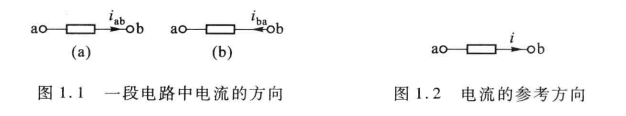
\includegraphics[width=0.72\textwidth]{1.1和1.2.png}
\end{figure}

分析复杂电路时往往难以判断电流的真实方向，而且有些电路中电流的真实方向随时间不断改变。为此，在列写电路方程时可任意假设一个方向，称为电流的\textbf{参考方向}，并用实线箭头标在图中。选定参考方向后，电流便是\textbf{代数量}：按参考方向求得的电流为正值，表明真实方向与参考方向一致；为负值则相反。电路的参考方向一经设定就不宜随意更改，否则极易导致符号混乱。

量值和方向不随时间变化的电流称为\textbf{直流}（DC），记作 $I$；随时间作周期性变化且平均值为零的电流称为\textbf{交变电流}（AC），记作 $i$ 或 $i(t)$。通常用大写字母表示直流，用小写字母表示随时间变化的量。

\subsection{电压}
单位正电荷从电路中一点移动到另一点，电场力对电荷做功。设电场力将电量为 $\mathrm{d}q$ 的正电荷由 $a$ 点移至 $b$ 点所做的功为 $\mathrm{d}W_{ab}$，则 $a$、$b$ 两点间的电压定义为
\begin{equation}
u_{ab}=\frac{\mathrm{d}W_{ab}}{\mathrm{d}q}
\end{equation}
电压的 SI 单位为伏[特]（$\mathrm{V}$）。

电压又称\textbf{电位差}。在电路中任选一点为参考点（零电位点，符号 $\perp$），某点与参考点之间的电压称为该点的\textbf{电位} $\varphi$，两点间的电压等于这两点的电位之差
\begin{equation}
u_{ab}=\varphi_a-\varphi_b
\end{equation}
电压的方向规定为从高电位指向低电位的方向，故电压有时也称为\textbf{电位降}。电压参考方向可用双下标、正负极性（$+$、$-$）或箭头三种方式表示，三者含义相同。

\corepoint{“电压”与“电位”的区别在于参考点：电位随参考点的选择而改变，两点间的电压与参考点无关。“电压降”与“电压升”只差一个符号，列 KVL 时统一按一种口径即可。}

\subsection{电动势}
电源具有将正电荷从低电位处经电源内部转移至高电位处的能力。设在 $\mathrm{d}t$ 时间内电源使正电荷 $\mathrm{d}q$ 从负极经电源内部移至正极所做的功为 $\mathrm{d}W'$，则电源的电动势定义为
\begin{equation}
e=\frac{\mathrm{d}W'}{\mathrm{d}q}
\end{equation}
即电动势的数值等于将单位正电荷从负极经电源内部移到正极时电源所做的功，其单位与电压相同。电动势的真实方向是把正电荷从低电位端移向高电位端的方向，因此\textbf{与电压的正方向刚好相反}。

\subsection{电功率}
电功率是衡量电能转换或传输速率的物理量。若在 $\mathrm{d}t$ 时间内消耗或吸收的能量为 $\mathrm{d}W$，则
\begin{equation}
p=\frac{\mathrm{d}W}{\mathrm{d}t}
\end{equation}
设某部分电路流过的电流为 $i$、端电压为 $u$，则 $\mathrm{d}t$ 内通过的电量为 $\mathrm{d}q=i\,\mathrm{d}t$，该电荷通过电路时电能所做的功 $\mathrm{d}W=u\,\mathrm{d}q=ui\,\mathrm{d}t$，于是这部分电路吸收的功率为
\begin{equation}
p=ui
\end{equation}
功率的 SI 单位为瓦[特]（$\mathrm{W}$），$1\,\mathrm{W}=1\,\mathrm{V}\times1\,\mathrm{A}$。

\textbf{关联参考方向}：同一元件上电压与电流的参考方向取成一致（电流从电压的“$+$”极流入），称为关联参考方向；否则称为非关联参考方向。功率的“吸收/发出”必须同时依据参考方向与计算结果的符号判定：

\begin{center}
\begin{tabular}{@{}lll@{}}
\toprule
参考方向 & 计算公式 & 结果为正时表示 \\
\midrule
关联 & $p=ui$ & 该部分电路\textbf{吸收}功率 \\
非关联 & $p=ui$ & 该部分电路\textbf{发出}功率 \\
\bottomrule
\end{tabular}
\end{center}

一段电路究竟是吸收还是发出功率，不会因参考方向选择不同而得出不同结论。例如某段电路 $u=-10\,\mathrm{V}$、$i=2\,\mathrm{A}$（关联），则 $p=-20\,\mathrm{W}<0$，说明它实际发出 $20\,\mathrm{W}$ 功率；若改取非关联方向，则 $u=10\,\mathrm{V}$、$p=20\,\mathrm{W}>0$，结论仍是发出 $20\,\mathrm{W}$。

功率等于能量的转换速率，在 $t_0\sim t$ 时间内电路吸收（关联参考方向）或发出（非关联参考方向）的能量为
\keyformula{W(t)=\int_{t_0}^{t}p(\xi)\,\mathrm{d}\xi=\int_{t_0}^{t}u(\xi)i(\xi)\,\mathrm{d}\xi}

实际电气设备、元器件本身都有功率限制，即\textbf{额定功率}。使用时实际功率不得超过额定值，否则（过载）会加速损耗甚至损坏设备。

\corepoint{功率计算的三步：（1）看 $u$、$i$ 是否关联；（2）按 $p=ui$ 算出代数值；（3）按上表由“参考方向＋符号”判定吸收或发出。千万不要见到负号就说“功率为负所以不消耗”。}

\section{电阻元件}
电阻元件是电阻器、白炽灯、电炉等实际器件的理想化模型，这些器件共同的特征是\textbf{消耗电能}。在电路理论中，将流过相同电流的两个端子称为一个\textbf{端口}。线性二端电阻的端口电压与电流之间遵循欧姆定律，二者成正比。在 $u$、$i$ 取关联参考方向时
\begin{equation}
u=Ri \qquad\text{或}\qquad i=Gu
\end{equation}
式中 $R$ 称为电阻[系数]，SI 单位为欧[姆]（$\Omega$），$1\,\Omega=1\,\mathrm{V}/1\,\mathrm{A}$；$G$ 称为电导[系数]，SI 单位为西[门子]（$\mathrm{S}$），$1\,\mathrm{S}=1\,\mathrm{A}/1\,\mathrm{V}$。若 $u$、$i$ 参考方向相反，两式中均应添一负号。

电阻与电导是反映同一电阻元件性能而互为倒数的两个参数
\begin{equation}
RG=1
\end{equation}

\begin{figure}[htbp]\centering
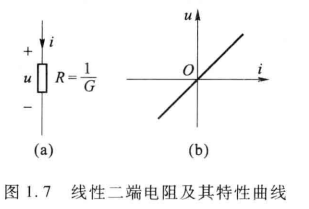
\includegraphics[width=0.5\textwidth]{1.7.png}
\end{figure}

线性电阻的端口特性在 $u-i$ 平面上是一条过原点的直线，称为电阻的电压电流关系曲线。$u$、$i$ 取关联参考方向且 $R$、$G$ 为正值时，特性曲线位于第 I、第 III 象限。

两种极端情况：
\begin{itemize}
  \item $R=0$：通过任意有限电流时电压恒为零，相当于\textbf{短路}（短路线电阻为零、电导为无穷大）；
  \item $G=0$：两端施加任意有限电压时电流恒为零，相当于\textbf{开路}（开路电导为零、电阻为无穷大）。
\end{itemize}

电阻吸收的功率为
\keyformula{p=ui=Ri^{2}=Gu^{2}}
若 $R$、$G$ 为正值，则 $p\ge 0$，这种电阻消耗电功率，属于\textbf{耗能元件}。从能量角度看，直到 $t$ 瞬间输入电阻的全部电能为
\begin{equation}
W=\int_{-\infty}^{t}p(\xi)\,\mathrm{d}\xi=\int_{-\infty}^{t}u(\xi)i(\xi)\,\mathrm{d}\xi
\end{equation}
此即物理学中的\textbf{焦耳定律}：导体或半导体电阻吸收电能并转化为热能。对于非负电阻，任一时刻该式结果非负，表明从全过程看这种元件只能吸收电能而不能发出电能——具有此种性质的元件称为\textbf{无源元件}。

若 $R<0$、$G<0$，关联参考方向下特性曲线位于第 II、第 IV 象限，电阻将输出电功率、对外提供电能，故\textbf{负电阻是一种有源元件}（可用电子线路实现，见第2章运放电路）。

从广义上讲，只要元件的端口电压、电流关系是代数方程，就属于电阻元件，其方程的一般形式为
\begin{equation}
u=u(i) \qquad\text{或}\qquad i=i(u)
\end{equation}
若 $u-i$ 关系不是过原点的直线，则称为\textbf{非线性电阻}。例如半导体二极管的电压电流关系为
\begin{equation}
i=I_0\left(\mathrm{e}^{u/U_T}-1\right)
\end{equation}
其中 $U_T$ 为热电压（常温下约 $26\,\mathrm{mV}$）。

\corepoint{判断“无源/有源”看的是元件能否对外提供能量：$R>0$ 时 $p=Ri^2\ge0$（无源），$R<0$ 时 $p<0$（有源）。这与“元件是否含电源”不是一回事。}

\section{电容元件}
电容元件是电容器的理想化模型，其电磁特性是\textbf{储存电荷与电场能量}。忽略损耗后，当极板间填充线性介质（介电常数与场强无关）时，电容储存的电荷 $q$ 与极板间电压 $u$ 成正比。若电压参考方向由正极板指向负极板，则线性电容的 $q-u$ 关系为
\begin{equation}
q=Cu
\end{equation}
式中 $C$ 为电容[系数]，单位 $\mathrm{C}/\mathrm{V}$，称为法[拉]（$\mathrm{F}$）。平行板电容器的电容为
\begin{equation}
C=\frac{\varepsilon A}{d}
\end{equation}
其中 $A$ 为每个极板的面积，$d$ 为极板间距，$\varepsilon$ 为介质的介电常数。$C$ 为常量的称为线性电容，否则为非线性电容。

\begin{figure}[htbp]\centering
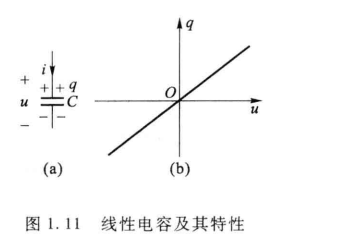
\includegraphics[width=0.55\textwidth]{1.11.png}
\end{figure}

当 $u$ 的参考方向由正极板指向负极板时，极板电荷的时间变化率就是端口电流，把 $q=Cu$ 代入得
\keyformula{i=C\frac{\mathrm{d}u}{\mathrm{d}t}}
即线性电容的端口电流与端口电压的\textbf{时间变化率}成正比。当端口施加直流电压时 $\mathrm{d}u/\mathrm{d}t=0$，端口电流为零，电容\textbf{等效成开路}。

反过来，电荷等于电流对时间的积分
\begin{equation}
q(t)=\int_{-\infty}^{t}i(\xi)\,\mathrm{d}\xi
\qquad\Longrightarrow\qquad
u(t)=\frac{1}{C}\int_{-\infty}^{t}i(\xi)\,\mathrm{d}\xi
\end{equation}
可见 $t$ 时刻电容上的电荷（电压）是此时刻以前电流充电、放电“积累”的结果，故电容具有记忆性质，属于\textbf{记忆元件}。把积分分成两段，得到常用的分段形式
\begin{equation}
u(t)=\frac{1}{C}\int_{-\infty}^{t_0}i(\xi)\,\mathrm{d}\xi+\frac{1}{C}\int_{t_0}^{t}i(\xi)\,\mathrm{d}\xi
=u(t_0)+\frac{1}{C}\int_{t_0}^{t}i(\xi)\,\mathrm{d}\xi
\end{equation}
式中 $u(t_0)$ 称为电容在 $t_0$ 时刻的\textbf{初始电压}，它代表了 $t_0$ 以前全部电流对电压的影响。

线性电容吸收的功率为 $p=ui=Cu\,\dfrac{\mathrm{d}u}{\mathrm{d}t}$。设 $t=-\infty$ 时电容尚未充电，$u(-\infty)=0$，则截止到 $t$ 时刻电容吸收的总能量为
\keyformula{W_e(t)=\frac{1}{2}Cu^{2}=\frac{q^{2}}{2C}}
这就是电容储存电场能量的计算公式。当 $u$ 的绝对值增大时 $p>0$（吸收能量），减小时 $p<0$（放出能量），故电容是\textbf{储能元件}，它不消耗能量，只是与电路交换能量。

\corepoint{电容三条推论必须记牢：（1）直流稳态下 $i=0$，电容相当于开路；（2）电容电压不能跃变（否则 $i=C\,\mathrm{d}u/\mathrm{d}t$ 将出现冲激，需无限大功率）；（3）$u$、$i$ 必须取关联参考方向，否则 $i=C\,\mathrm{d}u/\mathrm{d}t$ 前要加负号。}

\section{电感元件}
电感元件是电感线圈的理想化模型，其电磁特性是\textbf{储存磁链与磁场能量}，在周围激发磁场。若线圈的磁场存在于线性介质中，则磁链与电流成正比，称为线性电感；否则称为非线性电感。

设线性电感的磁链 $\Psi$ 与电流 $i$ 的参考方向符合右手螺旋定则，则
\begin{equation}
\Psi=Li
\end{equation}
式中 $L$ 为电感[系数]，磁链的单位为韦[伯]（$\mathrm{Wb}$），电流为安[培]时 $L$ 的 SI 单位为亨[利]（$\mathrm{H}$）。

\begin{figure}[htbp]\centering
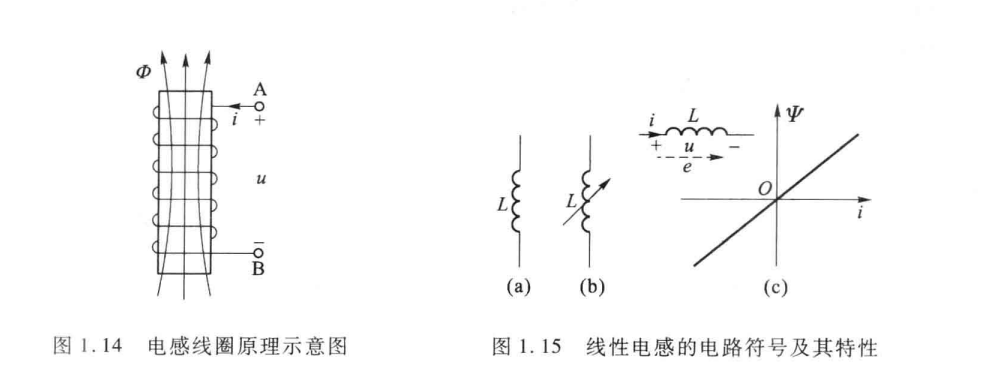
\includegraphics[width=0.5\textwidth]{1.14和1.15.png}
\end{figure}

根据电磁感应定律，磁链随时间的变化在电感中产生感应电动势 $e=-\dfrac{\mathrm{d}\Psi}{\mathrm{d}t}$。当 $u$、$e$ 与 $i$ 取关联参考方向且 $i$ 与 $\Psi$ 符合右手螺旋定则时
\begin{equation}
u=-e=-\left(-\frac{\mathrm{d}\Psi}{\mathrm{d}t}\right)=\frac{\mathrm{d}\Psi}{\mathrm{d}t}
\end{equation}
对线性电感代入 $\Psi=Li$ 得
\keyformula{u=L\frac{\mathrm{d}i}{\mathrm{d}t}}
即线性电感的端口电压与端口电流的\textbf{时间变化率}成正比。当电感中流过直流电流时 $\mathrm{d}i/\mathrm{d}t=0$，端口电压为零，电感\textbf{等效成短路}。

若由电压求磁链或电流，则需积分
\begin{equation}
\Psi(t)=\int_{-\infty}^{t}u(\xi)\,\mathrm{d}\xi=\Psi(t_0)+\int_{t_0}^{t}u(\xi)\,\mathrm{d}\xi,
\qquad
i(t)=i(t_0)+\frac{1}{L}\int_{t_0}^{t}u(\xi)\,\mathrm{d}\xi
\end{equation}
此二式表明电感中某一瞬间的磁链与电流决定于此瞬间以前的全部电压，故电感也是\textbf{记忆元件}。式中 $u$、$i$ 应为关联参考方向，否则需添负号。

线性电感吸收的功率为 $p=ui=Li\,\dfrac{\mathrm{d}i}{\mathrm{d}t}$，设 $t=-\infty$ 时 $i=0$，则截止到 $t$ 时刻电感吸收的能量为
\keyformula{W_m=\frac{1}{2}Li^{2}=\frac{\Psi^{2}}{2L}}
当电感电流的绝对值增大时 $p>0$（吸收能量并以磁场能形式储存），减小时 $p<0$（放出能量），故电感也是\textbf{储能元件}。

\corepoint{电感与电容完全对偶：$u\leftrightarrow i$、$L\leftrightarrow C$、$\Psi\leftrightarrow q$、短路 $\leftrightarrow$ 开路。记不住公式时按对偶关系推。}

三种基本无源元件的端口特性对照如下：
\begin{center}
\begin{tabular}{@{}lllll@{}}
\toprule
元件 & 特性方程 & 端口方程（关联） & 直流稳态 & 储能 \\
\midrule
电阻 & $u=Ri$ & $u=Ri$ & 有压有流 & 不储能（耗能） \\
电容 & $q=Cu$ & $i=C\dfrac{\mathrm{d}u}{\mathrm{d}t}$ & 开路 & $\frac{1}{2}Cu^{2}$ \\
电感 & $\Psi=Li$ & $u=L\dfrac{\mathrm{d}i}{\mathrm{d}t}$ & 短路 & $\frac{1}{2}Li^{2}$ \\
\bottomrule
\end{tabular}
\end{center}

\section{独立电源}
电源模型有电压源和电流源两种，它们的源电压或源电流与电路其他部分无关，故称为\textbf{独立电源}。

\subsection{电压源}
电压源能够提供确定的源电压 $u_s$。所谓“确定”是指 $u_s$ 与流过电压源的电流无关，而电压源的电流由与其相连的外电路决定。$u_s$ 为常量时称为直流电压源（恒定电压源），记作 $u_s=U_s$；也可以是时变量。源电压的方向从“$+$”极到“$-$”极。其端口特性为
\begin{equation}
u=u_s
\end{equation}
式中不含电流 $i$，表明源电压不受电流制约。$u_s$ 为常量时特性曲线是 $u-i$ 平面上平行于电流坐标轴的直线。当 $u_s=0$（电压源置零）时，其作用相当于\textbf{短路}。

按 $u$、$i$ 取非关联参考方向（电源内部从“$-$”到“$+$”），电压源发出的功率为
\begin{equation}
p=u_si
\end{equation}
$p>0$ 表示电源输出功率（供电），$p<0$ 表示电源吸收功率（充电）。

\subsection{电流源}
电流源能够提供确定的源电流 $i_s$，它与电流源端口电压无关，而端口电压由外电路决定。$i_s$ 为常量时记作 $i_s=I_s$。其端口特性为
\begin{equation}
i=i_s
\end{equation}
式中不含电压 $u$，特性曲线是平行于电压坐标轴的直线。当 $i_s=0$（电流源置零）时，其作用相当于\textbf{开路}。电流源输出的功率为 $p=ui_s$。

内阻 $R_i=0$ 的电压源与内导 $G_i=0$（内阻无穷大）的电流源分别称为\textbf{理想电压源}与\textbf{理想电流源}。由于零不能取倒数，理想电压源与理想电流源之间不能相互等效，是相互独立的两种电源模型（实际电源的两种模型及其等效变换见 §2.2）。

\corepoint{电压源置零 = 短路，电流源置零 = 开路，这两句是后面用叠加定理、戴维宁定理求等效电阻的基础，务必分清。另外“电压源不允许短路、电流源不允许开路”是理想电源的使用限制。}

\section{受控电源}
在电路模型中还要用到另一类电源，它们的源电压或源电流受电路中另一处的电压或电流控制，称为\textbf{受控电源}（非独立电源）。受控源是用来表示一条支路与另一条支路之间存在\textbf{耦合}关系的电路模型。本书只讨论线性受控源，即源电压（流）与控制电压（流）成正比。

控制量可以是电压或电流，被控制量也可以是电压或电流，故共有四种受控源：

\begin{center}
\begin{tabular}{@{}llll@{}}
\toprule
类型 & 简称 & 端口方程 & 控制系数量纲 \\
\midrule
电压控制电压源 & VCVS & $u_s=\mu u_c$ & 无量纲 \\
电流控制电压源 & CCVS & $u_s=r\,i_c$ & 电阻（$\Omega$） \\
电压控制电流源 & VCCS & $i_s=g\,u_c$ & 电导（$\mathrm{S}$） \\
电流控制电流源 & CCCS & $i_s=\beta\,i_c$ & 无量纲 \\
\bottomrule
\end{tabular}
\end{center}

式中带脚注 $s$ 的变量表示源，带脚注 $c$ 的变量表示控制量，$\mu$、$r$、$g$、$\beta$ 均为常量。

\begin{figure}[htbp]\centering
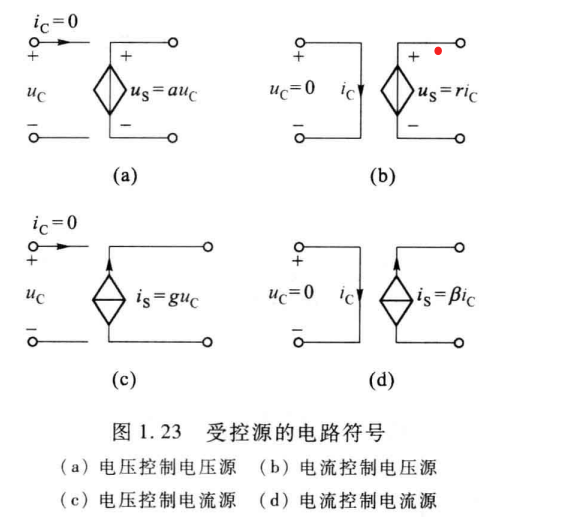
\includegraphics[width=0.72\textwidth]{1.23.png}
\end{figure}

受控源有两个端口，属\textbf{二端口元件}。由于它的控制量或是开路电压、或是短路电流，一般在电路图上不必专门画出控制端口，只需在菱形符号旁注明控制关系，并在电路中明确标注控制量即可。

受控源是电子线路中常用的电路模型。例如共射极接法的晶体管，其集电极电流 $i_c$ 与基极电流 $i_b$ 的关系为 $i_c=\beta i_b$，故其模型包含一个电流控制电流源。

\corepoint{受控源与独立源同属有源元件，但受控源本身不能提供能量：晶体管模型里受控源的能量归根结底来自外加直流电源。列写电路方程时，受控源先按独立源处理，再用待求量表示其控制量以消去中间变量（见第2章）。}

\section{基尔霍夫定律}
1847 年基尔霍夫建立了电路结构对电流、电压的约束关系，分别称为基尔霍夫电流定律（KCL）与基尔霍夫电压定律（KVL），统称基尔霍夫定律。

\subsection{电路结构}
电路结构用支路、节点、回路、网孔等术语描述。本书将每个二端元件称为一条\textbf{支路}；若干支路的连接点称为\textbf{节点}，其中两个支路的连接点称为\textbf{简单节点}。在节点 $a$ 到节点 $b$ 之间，由 $m$ 条不同支路和 $m-1$ 个不同节点（不含 $a$、$b$）依次连接成的一条通路称为 $a$ 到 $b$ 的\textbf{路径}，$a$、$b$ 分别称为始端节点和终端节点。

闭合的路径称为\textbf{回路}，回路有顺时针、逆时针两个方向。将电路画在平面上，若除节点外各支路都不相交，则称为\textbf{平面电路}，否则称为非平面电路。平面电路的单孔回路（内部或外部不包含任何支路）称为\textbf{网孔}，它是最简单的回路；内部不含支路的网孔称为内网孔，外部不含支路的称为外网孔，若无特别说明网孔均指内网孔。

一条支路若不管电流为何有限值电压恒等于零，则称为\textbf{短路}；若不管电压为何有限值电流恒等于零，则称为\textbf{开路}（断路）。

\begin{figure}[htbp]\centering
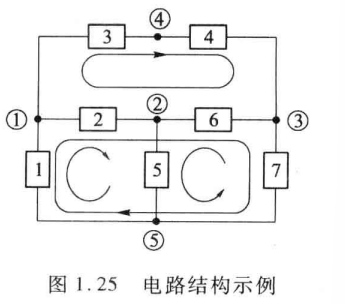
\includegraphics[width=0.62\textwidth]{1.25.png}
\end{figure}

\subsection{基尔霍夫电流定律}
\textbf{KCL}：在集中参数电路中，任一时刻流出（或流入）任一节点的支路电流的代数和等于零，即
\keyformula{\sum_{k=1}^{b} i_k=0}
通常规定：$i_k$ 的参考方向为\textbf{流出}节点时前面取“$+$”号，流入节点时取“$-$”号。该式称为节点的 KCL 方程，它反映了与任一节点相连的所有支路电流所满足的约束。

KCL 还可推广用于闭合边界，称为\textbf{广义基尔霍夫电流定律}：在集中参数电路中，任一时刻流出（或流入）任一闭合边界 $S$ 的支路电流的代数和等于零
\begin{equation}
\sum_{\text{流出}S} i_k=0
\end{equation}
由于流入任一节点的电流代数和为零，把闭合边界内各节点的 KCL 方程相加即得广义 KCL。由此还可得等价表述：任一时刻，流出任一节点（或闭合边界）电流的代数和等于流入该节点电流的代数和
\begin{equation}
\sum i_{\text{出}}=\sum i_{\text{入}}
\end{equation}

独立性：含有 $n$ 个节点的电路中，任意 $n-1$ 个节点的 KCL 方程是一组独立方程，这些节点称为\textbf{独立节点}；第 $n$ 个节点的 KCL 方程必是其余 $n-1$ 个方程的代数和。至于选哪 $n-1$ 个节点作独立节点则是任意的。

\subsection{基尔霍夫电压定律}
\textbf{KVL}：在集中参数电路中，任一时刻沿任一回路各支路电压的代数和等于零，即
\keyformula{\sum_{k=1}^{b} u_k=0}
通常规定：$u_k$ 的参考方向与回路方向\textbf{相同}时前面取“$+$”号，否则取“$-$”号。该式称为回路的 KVL 方程，它是任一回路所包含的支路电压必须满足的约束。

推广形式一：沿任一回路，各支路\textbf{电压降}的代数和等于\textbf{电压升}的代数和
\begin{equation}
\sum u_{\text{降}}=\sum u_{\text{升}}
\end{equation}
教材中常见写法为 $\sum u=0$（绕行一周电压降之和为零）与 $\sum u_{\text{升}}=0$ 两种口径，二者只差一个符号。

推广形式二：集中参数电路中，\textbf{任意两点之间的电压具有确定值，与计算路径无关}（即电压与路径无关，只与两端点有关）。这一性质是把“两点间电压”写成“沿某条路径的电压降之和”的依据。

设电路有 $b$ 条支路、$n$ 个节点，则独立 KVL 方程的个数（独立回路数）为
\begin{equation}
m=b-(n-1)
\end{equation}
对平面电路的全部内网孔列出的 KVL 方程必是一组独立方程；反之，任一网孔的 KVL 方程不能表示为其余网孔 KVL 方程的线性组合。取网孔只是获得独立 KVL 方程的\textbf{充分条件}而非必要条件，例如“两个网孔＋一个非网孔回路”也可以是独立组，但独立方程的数目总是一样的。

\corepoint{基尔霍夫定律只与电路结构有关，\textbf{与元件性质无关}：无论元件是线性还是非线性、含源还是无源、时变还是非时变，KCL、KVL 都成立；KVL 还可用于含“假想支路”（断开处）的假想回路。这正是它被称为“结构约束”的原因。}

\subsection{两类约束与列方程的思路}
列写电路方程时，KCL 约束的是与节点相连的支路电流，KVL 约束的是回路所包含的支路电压，二者提供的独立方程数为 $(n-1)+[b-(n-1)]=b$；再与 $b$ 个支路的元件方程联立，即可解出 $b$ 个支路电流（或电压）。这一思路在下一章发展为支路电流法、回路电流法和节点电压法。

\begin{center}
\begin{tabular}{@{}lll@{}}
\toprule
约束类型 & 依据 & 独立方程数 \\
\midrule
结构约束（KCL） & 节点电流代数和为零 & $n-1$ \\
结构约束（KVL） & 回路电压代数和为零 & $b-(n-1)$ \\
元件约束 & 各元件端口方程 & $b$ \\
\bottomrule
\end{tabular}
\end{center}

\endinput

% 电路与电子学III 课程笔记 —— 第2章（教材：孙立山《电路理论基础》第四版 第2章）
\chapter{线性直流电路}

\noindent
由直流电压源和（或）直流电流源激励，且各部分电压、电流都是恒定量的电路称为\textbf{直流电路}；由线性元件和独立源组成的直流电路称为\textbf{线性直流电路}，它是最简单、最基本的一类电路。本章内容分三部分：（1）\textbf{等效化简}——等效的概念、电阻串并联与星形三角形变换、含源支路的等效变换；（2）\textbf{一般分析方法}——支路电流法、回路电流法、节点电压法；（3）\textbf{运算放大器}及其电路的分析。

\section{电阻网络的等效}
若干电阻相互连接构成的电路称为\textbf{电阻网络}。所谓\textbf{等效}，是指被化简的网络与等效网络具有相同的对应端口特性，即端口 $u-i$ 关系方程相同。用等效网络代替原网络后，\textbf{不改变其余部分}（外电路）的电压和电流。

\corepoint{“等效”只对外电路成立，对内不等效：等效前后被替换部分内部的电压、电流、功率一般都会改变（例如电压源与电阻并联等效成电压源后，电阻上的电流与功率都不一样了）。这是判断“能不能这样等效”的第一原则。}

\subsection{电阻的串联}
当各电阻首尾依次连接、连接点处没有分支，由 KCL 可知各电阻流过相同电流，则称这些电阻为\textbf{串联}。由 KVL 及欧姆定律
\begin{equation}
u=R_1i+R_2i=(R_1+R_2)i=R_{eq}i
\end{equation}
故两个电阻串联的等效电阻为 $R_{eq}=R_1+R_2$；$n$ 个电阻串联时
\keyformula{R_{eq}=\sum_{k=1}^{n}R_k}
串联常用于\textbf{分压}，各电阻上的电压为
\keyformula{u_k=\frac{R_k}{R_{eq}}\,u}
两个电阻串联时分压公式为 $u_1=\dfrac{R_1}{R_1+R_2}u$，$u_2=\dfrac{R_2}{R_1+R_2}u$。串联时流过相同电流，各电阻消耗的功率 $p_k=R_ki^2$，故
\begin{equation}
\frac{u_1}{u_2}=\frac{p_1}{p_2}=\frac{R_1}{R_2}
\end{equation}
即\textbf{串联时各电阻上的电压和功率的分配均与电阻成正比}。

注意：某些情况下电阻并非依次连接，但只要通过相同的电流，也可按串联化简。但这种变换后若把参考点选在被变换部分内部，未变换部分的节点电压会改变，严格说来不能称为等效变换。

\subsection{电阻的并联}
若各电阻都接到同一对节点之间、承受相同电压，则称这些电阻为\textbf{并联}。由 KCL 及欧姆定律
\begin{equation}
i=\frac{u}{R_1}+\frac{u}{R_2}=(G_1+G_2)u=G_{eq}u
\end{equation}
故两个电阻并联的等效电导为 $G_{eq}=G_1+G_2$，等效电阻为 $R_{eq}=\dfrac{R_1R_2}{R_1+R_2}$；$n$ 个电阻并联时
\keyformula{G_{eq}=\sum_{k=1}^{n}G_k,
\qquad
\frac{1}{R_{eq}}=\sum_{k=1}^{n}\frac{1}{R_k}}
并联常用于\textbf{分流}，各电阻分得的电流为
\keyformula{i_k=\frac{G_k}{G_{eq}}\,i}
两个电阻并联时分流公式为 $i_1=\dfrac{R_2}{R_1+R_2}i$，$i_2=\dfrac{R_1}{R_1+R_2}i$。并联时承受相同电压，$p_k=G_ku^2$，故
\begin{equation}
\frac{i_1}{i_2}=\frac{p_1}{p_2}=\frac{G_1}{G_2}
\end{equation}
即\textbf{并联时各电阻上的电流和功率的分配均与电导成正比}。

\corepoint{串联看电阻（分压、功率与 $R$ 成正比），并联看电导（分流、功率与 $G$ 成正比）。两个电阻并联时“积除和”$R_1R_2/(R_1+R_2)$ 要背熟；$n$ 个相等电阻 $R$ 并联的等效电阻为 $R/n$。}

\subsection{电阻的星形联结和三角形联结}
电阻的星形联结简称 $Y$ 形联结或 $T$ 形联结；三角形联结简称 $\Delta$ 形联结或 $\pi$ 形联结。在一定条件下二者可以相互等效，用以实现网络的等效化简——典型场合是\textbf{电桥电路}，它不能用串并联等效直接计算等效电阻。

$Y$ 形与 $\Delta$ 形都是\textbf{三端网络}：有三对端子间电压 $u_{12}$、$u_{23}$、$u_{31}$ 和三个端子电流 $i_1$、$i_2$、$i_3$。由 KCL、KVL 恒有 $i_1+i_2+i_3=0$、$u_{12}+u_{23}+u_{31}=0$，故三端网络的对外作用可用两对端子间电压与两个端子电流的关系表示。令两种联结的对应端口特性方程系数相等，即得等效条件。

$\Delta$ 形联结到 $Y$ 形联结的等效变换公式为
\keyformula{R_1=\frac{R_{12}R_{31}}{R_{12}+R_{23}+R_{31}},\quad
R_2=\frac{R_{23}R_{12}}{R_{12}+R_{23}+R_{31}},\quad
R_3=\frac{R_{31}R_{23}}{R_{12}+R_{23}+R_{31}}}
可归纳为
\begin{equation}
R_{1,2,3}=\frac{\Delta\text{形联结中与该节点相连两电阻之积}}{\Delta\text{形联结中各电阻之和}}
\end{equation}
$Y$ 形联结到 $\Delta$ 形联结的等效变换公式为
\keyformula{R_{12}=\frac{R_1R_2+R_2R_3+R_3R_1}{R_3},\quad
R_{23}=\frac{R_1R_2+R_2R_3+R_3R_1}{R_1},\quad
R_{31}=\frac{R_1R_2+R_2R_3+R_3R_1}{R_2}}
可归纳为
\begin{equation}
R_{12,23,31}=\frac{Y\text{形联结各电阻两两乘积之和}}{Y\text{形联结中不相邻的电阻}}
\end{equation}

对称情况最简单常用：设三个相等电阻接成 $Y$ 形或 $\Delta$ 形，则
\keyformula{R_{\Delta}=3R_{Y},\qquad R_{Y}=\frac{1}{3}R_{\Delta}}
以上分析表明：对称 $Y$ 形联结等效为 $\Delta$ 形联结时也是对称的，反之亦然。

\corepoint{$Y$-$\Delta$ 变换的三个电阻必须“有公共节点”（$Y$）或“构成回路”（$\Delta$）才能用；变换时先标清三个端子的对应关系，再代公式，端子标错是最常见的错误。对称情形 $R_\Delta=3R_Y$ 可以快速验算。}

\section{含源支路的等效变换}
两种典型的含独立源一端口电路，在端口电压、电流取\textbf{非关联}参考方向的条件下，其电压电流关系分别为
\keyformula{U=U_s-R_iI,\qquad I=I_s-G_iU}
当电路参数满足一定条件时，\textbf{电压源和电阻串联支路与电流源和电导并联支路可以相互等效}。将第二式改写为
\begin{equation}
U=\frac{1}{G_i}I_s-\frac{1}{G_i}I
\end{equation}
与第一式比较，得两电路的等效变换条件
\keyformula{U_s=\frac{I_s}{G_i},\qquad R_i=\frac{1}{G_i}}
即 $U_s=I_sR_i$，$I_s=U_s/R_i$。

物理意义：实际稳压电源工作时，随端口电流变化，其端口电压也略有变化，故用“电压源＋电阻串联”作模型——$U_s$ 是空载（输出电流为零）时的输出电压，$R_iI$ 是由负载电流引起的输出电压降，$R_i$ 称为电源的等效内电阻。实际稳流电源则用“电流源＋电导并联”作模型——$I_s$ 是空载（输出电压为零即短路）时的输出电流，$G_iU$ 是由负载电压引起的输出电流下降，$G_i$ 称为内导。因此实际电源都有这两种等效的电路模型。

几种特殊连接：
\begin{itemize}
  \item 电压源与电阻\textbf{并联}的一端口，其端口电压恒为 $U_s$、电流不确定，对外作用等效为电压源 $U_s$（电阻可去掉）；
  \item 电流源与电阻\textbf{串联}的一端口，其端口电流恒为 $I_s$，对外作用等效为电流源 $I_s$（电阻可去掉）；
  \item 两个电压源串联、两个电流源并联，可直接按代数和合并；两个相同电压源并联、两个相同电流源串联，等效为一个同值电源。
\end{itemize}

受控电压源与电阻的串联也可等效成受控电流源与同一电阻的并联，或反之，变换方法与含独立源的情况相似；\textbf{但在变换过程中应保证控制量的位置不变}。

\corepoint{理想电压源（$R_i=0$）与理想电流源（$G_i=0$）之间\textbf{不能}相互等效，因为零不能取倒数。凡涉及理想电源的等效变换，都要先问“内阻是不是零”。}

\section{支路电流法}
能用等效化简分析的电路通常是结构较简单、只求个别量的电路。当电路复杂以致难以化简，或待求变量较多时，就要依据电路变量的基本约束列写方程组求解。

设电路有 $b$ 条支路、$n$ 个节点，各独立源、受控源和电阻的参数均已知，要求确定各支路电流或电压。\textbf{支路电流法}就是以 $b$ 条未知的支路电流为待求量：

\begin{enumerate}
  \item 设定各支路电流的参考方向，并标在电路图上；
  \item 对 $n-1$ 个独立节点列写 KCL 方程；
  \item 对 $b-(n-1)$ 个独立回路列写 KVL 方程，其中电阻电压用支路电流表示；
  \item 联立 $b$ 个方程求解，再按需由支路电流求其他量。
\end{enumerate}

支路电流法是分析电路的一种基本方法，正确运用的关键在于所列 $b$ 个方程\textbf{彼此独立}：$n-1$ 个节点的 KCL 方程是一组独立方程；为列独立的 KVL 方程，可每选一个回路时\textbf{至少包括一条新支路}，从而在该回路的 KVL 方程中包含一个新的支路电压，使方程独立于已列出的方程。

含电流源电路的处理：把电流源支路的电流视为已知，列 KCL 时可将其直接移到等号右端；对含电流源的回路列 KVL 时，须把未知的电流源端电压列入方程（多一个未知量、多一个补充方程），或\textbf{适当选取回路使所取回路不包含电流源}，从而减少方程数目。

含受控源电路的处理：在支路电流方程中，受控源先按独立源处理，再用支路电流表示其控制电压（流），代入后消去控制量。

\corepoint{支路电流法的方程数等于支路数 $b$，未知量最多、计算量最大，但思路最直接、不易出错，适合作为检验其他方法的基准。含电流源时“选回路绕开它”能立刻少一个方程。}

\section{回路电流法}
支路电流法的待求量数目等于未知支路电流数，所需方程较多。若以假想的回路电流为待求量，则可大幅减少方程数。

\subsection{回路电流}
由于电流具有连续性，可以假设在每个独立回路中分别存在一个闭合流动的电流，这就是\textbf{回路电流}；以网孔为回路时也称为\textbf{网孔电流}。假设回路电流后，支路电流便可用回路电流的代数和表示：若支路电流与回路电流方向相同，回路电流前取正号，否则取负号。

以回路电流为待求量便\textbf{等价地应用了 KCL}——把支路电流用回路电流表示后代入任一节点的 KCL 方程，得到的是恒等于零的恒等式。因此回路电流法\textbf{无需再列 KCL 方程}。

\subsection{回路电流方程的列写}
选择 $b-(n-1)$ 个独立回路，以各回路电流为待求量列写 KVL 方程，这种方法称为\textbf{回路电流法}（回路分析法）。其标准形式为
\keyformula{\begin{aligned}
R_{11}I_{m1}+R_{12}I_{m2}+\cdots+R_{1m}I_{mm}&=U_{s11}\\
R_{21}I_{m1}+R_{22}I_{m2}+\cdots+R_{2m}I_{mm}&=U_{s22}\\
&\vdots\\
R_{m1}I_{m1}+R_{m2}I_{m2}+\cdots+R_{mm}I_{mm}&=U_{smm}
\end{aligned}}
各项意义与列写规则：
\begin{enumerate}
  \item \textbf{自阻} $R_{kk}$：组成第 $k$ 个回路的各支路电阻之和，恒取正号；
  \item \textbf{互阻} $R_{kj}$（$k\neq j$）：第 $k$、$j$ 两回路公共支路上的电阻。若两回路电流在该公共支路上方向\textbf{相同}，互阻取正；\textbf{相反}取负。在仅由独立源和二端电阻组成的电路中 $R_{kj}=R_{jk}$，即系数矩阵\textbf{对称}；
  \item 等号右边 $U_{skk}$：沿第 $k$ 个回路方向各电压源\textbf{电位升}的代数和（电位升取正、电位降取负）。
\end{enumerate}
写成矩阵形式 $\boldsymbol{RI}_m=\boldsymbol{U}_s$，其中 $\boldsymbol{I}_m$ 称为回路电流向量，$\boldsymbol{U}_s$ 称为回路源电压向量，系数矩阵称为回路电阻矩阵。

含电流源电路：方法一是以网孔为独立回路，把电流源两端未知电压 $U$ 列入方程，再补充电流源的特性方程；方法二是\textbf{适当选取独立回路使电流源只包含在一个回路中}，则该回路电流即等于源电流 $I_s$，从而减少一个待求量及方程数。后者显然更优。

含受控源电路：先用回路电流表示受控源的控制量，代入消去控制量后整理。此时受控源的控制系数要影响方程的系数，通常使系数矩阵\textbf{不再具有对称性}。

\corepoint{回路电流法的三个易错点：（1）自阻恒正、互阻看方向；（2）等号右边是“电位升”的代数和（沿回路方向从“$-$”到“$+$”取正）；（3）含电流源时要主动选回路，让电流源独占一个回路。}

\section{节点电压法}
在集中参数电路中任选一节点为\textbf{参考点}，其他各节点与参考点之间的电压称为该节点的\textbf{节点电压}（节点电位）；参考点的节点电压为零。有了节点电压，任意两点间电压便可表达成这两个节点电压之差。

用节点电压表示支路电压，相当于\textbf{等价地列写了 KVL 方程}——绕任一回路一周，各节点电压相互抵消，方程恒等于零。因此以节点电压为待求量时\textbf{无需再列 KVL 方程}。以 $n-1$ 个节点电压为待求量、对 $n-1$ 个节点列写 KCL 方程的方法，就是\textbf{节点电压法}（节点分析法）。

其标准形式为
\keyformula{\begin{aligned}
G_{11}U_{n1}+G_{12}U_{n2}+\cdots+G_{1,n-1}U_{n,n-1}&=I_{s11}\\
G_{21}U_{n1}+G_{22}U_{n2}+\cdots+G_{2,n-1}U_{n,n-1}&=I_{s22}\\
&\vdots
\end{aligned}}
列写规则：
\begin{enumerate}
  \item \textbf{自导} $G_{kk}$：与节点 $k$ 直接相连的各支路电导之和，恒取正号；
  \item \textbf{互导} $G_{kj}$（$k\neq j$）：直接连接在节点 $k$、$j$ 之间的诸支路电导之和并\textbf{带负号}。在仅由独立源和线性二端电阻组成的电路中 $G_{kj}=G_{jk}$，系数矩阵\textbf{对称}；
  \item 等号右边 \textbf{节点源电流} $I_{skk}$：包括两项——（1）与节点 $k$ 相连的各电流源电流的代数和（电流\textbf{流入}节点取正，流出取负）；（2）与节点 $k$ 相连的各“电压源与串联电导”的乘积 $G U_s$ 的代数和（电压源\textbf{正极性端指向}该节点时取正，否则取负）。
\end{enumerate}
写成矩阵形式 $\boldsymbol{GU}_n=\boldsymbol{I}_s$，$\boldsymbol{U}_n$ 为节点电压向量，$\boldsymbol{I}_s$ 为节点源电流向量，系数矩阵为节点电导矩阵。复杂电路中节点电导矩阵元素大部分为零，属于\textbf{稀疏矩阵}，计算时要用稀疏矩阵技术。

只有一个独立节点（多条支路并联）时，节点电压可直接写出
\begin{equation}
U_{n1}=\frac{\sum I_s+\sum GU_s}{\sum G}
\end{equation}
即“注入电流的代数和 ÷ 各支路电导之和”，这就是\textbf{弥尔曼定理}。

\subsection{改进节点电压法}
上述节点电压法是根据欧姆定律用节点电压表示二端电阻的电流。若电路中存在\textbf{非二端电阻元件}（如纯电压源支路），该支路电流不能用支路电导与节点电压之积表示。解决办法有两种：

\begin{enumerate}
  \item \textbf{改进节点法}：以 $n-1$ 个节点电压和纯电压源支路的电流为待求量，列 $n-1$ 个节点的 KCL 方程，再与纯电压源支路的方程（$U_{nk}-U_{nj}=U_s$）联立；
  \item 若电路中只有一个纯电压源支路，可\textbf{选电压源的一端为参考点}，则另一端的节点电压即为已知量，问题大为简化——此时只需对其余节点列 KCL，且未知的电压源电流只出现在被略去的那个方程中。
\end{enumerate}

\corepoint{三种方法对比：支路电流法 $b$ 个方程（最直观）；回路电流法 $b-n+1$ 个方程（自阻互阻规则稍繁）；节点电压法 $n-1$ 个方程（自导互导规则最简单，便于编程）。因为节点电压法的列写规则比回路电流法简单，工程与仿真软件（PSPICE 等）普遍采用节点电压法。}

\begin{center}
\begin{tabular}{@{}llll@{}}
\toprule
方法 & 待求量 & 方程数 & 方程类型 \\
\midrule
支路电流法 & $b$ 个支路电流 & $b$ & $n-1$ 个 KCL $+\,b-n+1$ 个 KVL \\
回路电流法 & $b-n+1$ 个回路电流 & $b-n+1$ & 仅 KVL \\
节点电压法 & $n-1$ 个节点电压 & $n-1$ & 仅 KCL \\
\bottomrule
\end{tabular}
\end{center}

\section{运算放大器}
运算放大器（简称运放）是用集成电路工艺制成的\textbf{多端元件}，其内部电路分析超出本课程范围。由于它具有对输入信号进行求和、放大、积分、微分等运算功能，故得此名。

\subsection{端口特性}
仅从外部端子分析，运放是一种高放大倍数的电压放大器。用 $u_+$、$u_-$ 分别表示同相输入端和反相输入端的节点电压，则输入端口电压即\textbf{差分输入电压}为
\begin{equation}
u_d=u_+-u_-
\end{equation}
在输出端开路情况下，输出电压 $u_o$ 与差分输入电压的关系曲线可用折线近似：水平部分称为运放的\textbf{饱和区}，中间部分（$-U_{cc}<u_d<+U_{cc}$）为\textbf{线性区}，在此区域内输出电压与输入电压成正比。二者之比称为\textbf{开环增益}（开环电压放大倍数）$A$，即 $u_o=Au_d$。

本书只讨论运放工作在\textbf{线性区}时的功能与分析方法。线性区内运放的电路模型由输入电阻 $R_i$、输出电阻 $R_o$ 和受控电压源 $Au_d$ 组成（含受控源，说明运放是有源元件）。典型参数：开环增益 $A\sim10^{5}$、输入电阻 $R_i\sim10^{6}\sim10^{13}\,\Omega$、输出电阻 $R_o\sim10\sim100\,\Omega$，工作电压 $\pm5\sim\pm24\,\mathrm{V}$。

由于开环增益非常大，一个微小的输入电压就足以使运放进入饱和区。因此为使运放工作在线性区，\textbf{必须引入负反馈}——将输出电压或输出电压的一部分回馈到反相输入端；若回馈到同相输入端则属正反馈。

\subsection{理想运算放大器}
仅分析电路工作原理时常用\textbf{理想运放}模型，其条件是：无穷大的开环增益、无穷大的输入电阻和零输出电阻。由此得到理想运放的端口特性
\keyformula{i_+=i_-=0,\qquad u_+=u_-}
其中 $i_+$、$i_-$ 为两个输入端的电流。这两个式子不含理想运放的输出电压 $u_o$ 和输出电流 $i_o$，它们将由外接电路决定。

第一式表明输入端口电流为零，类似于\textbf{断路}，称为\textbf{虚断}；第二式表明输入端口电压为零，又类似于\textbf{短路}，称为\textbf{虚短}。故可以说理想运放输入端口满足“虚断”和“虚短”条件。

\corepoint{“虚短、虚断”是分析含理想运放电路的唯一钥匙，但两者都\textbf{以负反馈为前提}：没有负反馈时运放工作在饱和区，$u_+\neq u_-$，虚短不成立。判断电路是否含负反馈，是做题的第一步。}

\section{含运算放大器电路的分析}
理想运放输入端口电压、电流均为零，而输出端口电压、电流取决于运放之外的电路，这些特性决定了分析方法的特殊性。

\subsection{反相放大器}
输入电压经 $R_1$ 接反相输入端，$R_f$ 从输出端接回反相输入端，同相输入端接地。由虚断 $i_+=i_-=0$ 得 $i_1=i_f$；由虚短 $u_-=u_+=0$（\textbf{虚地}）有 $\dfrac{u_1-0}{R_1}=\dfrac{0-u_o}{R_f}$，于是得
\keyformula{u_o=-\frac{R_f}{R_1}u_1}
可见输出电压与输入电压成正比、极性相反，故称反相放大器。其增益只与\textbf{外接电阻}有关，故可实现高精度、高稳定性的增益值。反相输入端电位近似为零但不接地，称为“虚地”。

\subsection{同相放大器}
输入电压加在同相输入端，反相输入端经 $R_1$ 接地、经 $R_f$ 接输出端。由虚短 $u_-=u_+=u_1$，再由虚断 $i_1=i_f$ 及分压关系得
\keyformula{u_o=\left(1+\frac{R_f}{R_1}\right)u_1}
它是增益大于 1 的电压控制电压源，输出电压与输入电压极性相同。若令 $R_1=\infty$、$R_f=0$，则 $u_o=u_1$，电路成为\textbf{电压跟随器}，常在多级电路中起隔离作用——它从输入电压源吸收的电流为零，即输入电压源不提供功率。

\subsection{加法器}
三个输入电压经 $R_1$、$R_2$、$R_3$ 接反相输入端，$R_f$ 接回输出端。由虚短得 $u_-=0$，由虚断得 $i_1+i_2+i_3=i_f$，于是
\keyformula{u_o=-\left(\frac{R_f}{R_1}u_1+\frac{R_f}{R_2}u_2+\frac{R_f}{R_3}u_3\right)}
即输出电压是输入电压的\textbf{线性组合}（加权和），各系数称为加权系数。若 $R_1=R_2=R_3=R_f$，则各加权系数相等为 $-1$，$u_o=-(u_1+u_2+u_3)$。

\subsection{差分放大器}
同时从两个输入端加入输入电压，便构成差分放大器。由虚短、虚断并利用分压公式与 KVL 可求得
\begin{equation}
u_o=\frac{R_2}{R_1}\left(1+\frac{R_1}{R_2}\right)\frac{R_4}{R_3+R_4}u_2-\frac{R_2}{R_1}u_1
\end{equation}
若外接电阻满足平衡条件 $\dfrac{R_2}{R_1}=\dfrac{R_4}{R_3}$，则化简为
\keyformula{u_o=\frac{R_2}{R_1}\left(u_2-u_1\right)}
即输出电压与两输入电压之差成正比。差分放大器的主要优点是：若两个输入电压因干扰受到\textbf{相同}的扰动（共模信号），则该扰动不会影响输出电压。

\subsection{用运放实现负电阻}
利用运放可以把正电阻变换为\textbf{等效负电阻}：按虚断、虚短列方程，可得端口等效电阻为负值（$R_{eq}<0$）。负电阻是有源元件，能对外发出功率，这与 §1.2 的结论一致。

\subsection{复杂含运放电路的分析}
上述只涉及简单电路。电路较复杂时需列写联立方程组，在各种方法中\textbf{节点电压法}是分析含运放电路的有效方法：把运放的两个输入端当作普通节点列 KCL（因虚断，输入端电流为零，两节点之间不存在互导），再补充理想运放的端口方程 $u_+=u_-$ 作为约束。运放的输出电流只出现在输出节点的 KCL 方程中，若不需要求它，可略去输出节点的 KCL 方程。

\corepoint{含运放电路的分析套路：（1）确认存在负反馈；（2）对输入端节点写 KCL（虚断使输入端不“吃掉”电流）；（3）补 $u_+=u_-$（虚短/虚地）；（4）解出输出与输入的关系。求输出电流时，输出节点的 KCL 方程不可略。}

\section{对偶原理}
（本节内容在教材中位于第 3 章 3.6 节，因与本章的回路法、节点法直接对偶，故提前介绍。）

如果两个电路的方程互为对偶，则称这两个电路\textbf{互为对偶}。把电路中的变量和参数按对偶关系替换，方程形式不变，这一规律称为\textbf{对偶原理}。常用对偶关系如下：

\begin{center}
\begin{tabular}{@{}llll@{}}
\toprule
电压 $u$ & 电流 $i$ & 电阻 $R$ & 电导 $G$ \\
电荷 $q$ & 磁链 $\Psi$ & 电容 $C$ & 电感 $L$ \\
电压源 $u_s$ & 电流源 $i_s$ & 开路 & 短路 \\
串联 & 并联 & 节点 & 网孔（回路） \\
KCL & KVL & 节点电压法 & 回路电流法 \\
$Y$ 形联结 & $\Delta$ 形联结 & 自导 & 自阻 \\
\bottomrule
\end{tabular}
\end{center}

应用要点：
\begin{enumerate}
  \item 对偶是\textbf{方程层面}的对应关系，两个互为对偶的电路其结构图互为“对偶图”——原电路的网孔对应对偶电路的节点，反之亦然；
  \item 已知一个电路的结论，按对偶关系逐项替换即得对偶电路的结论（例如由分压公式 $u_k=R_k/R_{eq}\cdot u$ 立即得到分流公式 $i_k=G_k/G_{eq}\cdot i$）；
  \item 对偶关系要求参考方向也作相应约定，否则会差一个负号。
\end{enumerate}

\corepoint{对偶原理是“少背一半公式”的工具：串并联、分压分流、$Y$-$\Delta$、回路法与节点法、$RL$ 与 $RC$ 暂态，全都可以两两对偶记忆。但要记住它只对方程与结构成立，不是物理上的等价。}

\endinput

% 电路与电子学III 课程笔记 —— 第3章（教材：孙立山《电路理论基础》第四版 第3章）
\chapter{电路定理}

\noindent
本章介绍电路理论中几个常用定理。\textbf{置换定理}适用于线性与非线性电路；\textbf{齐性定理}和\textbf{叠加定理}体现线性电路的本质，是线性方程的齐次性与可加性在电路中的体现；\textbf{戴维宁定理}和\textbf{诺顿定理}（合称等效电源定理）是化简线性含源一端口电路的有效方法；\textbf{特勒根定理}与基尔霍夫定律同样普遍适用，并可用以证明\textbf{互易定理}；对偶原理见 §2.8。

\section{置换定理}
\textbf{置换定理}：在任意线性和非线性电路中，若已知某一端口的电压和电流分别为 $U$ 和 $I$，则可用 $U_S=U$ 的电压源或 $I_S=I$ 的电流源来置换此一端口，而\textbf{不影响电路中其他部分}的电压和电流。

证明思路（图示法）：设一端口 $N_1$ 与 $N_2$ 的端口特性分别为 $U=f_1(I)$ 与 $I=f_2(U)$，把它们画在 $u-i$ 平面上，两曲线交点的坐标 $(U,I)$ 即端口的解。置换时用源电压等于该解的电压源（其图像是平行于 $i$ 轴的直线）代替 $N_2$，由于置换前后 $N_1$ 的结构与参数均未改变，$f_1(\cdot)$ 曲线不变，而端口电压仍为 $U$，故端口电流仍为 $I$——$N_1$ 内部各电压、电流均不受影响。用电流源置换的论证类似。

应用置换定理时必须注意两点：
\begin{enumerate}
  \item 置换后的电路必须\textbf{有唯一解}（实际电路与大多数电路模型都满足）；
  \item 除被置换部分发生变化外，\textbf{其余部分在置换前后必须保持完全相同}。
\end{enumerate}

由置换定理可得两个常用\textbf{推论}：
\begin{itemize}
  \item 若电路中某两点间电压为零，则可将量值为零的电压源接于该两点间，相当于把这两点\textbf{短路}，短路后不影响其他部分的解答；
  \item 若电路中某支路电流为零，则可将量值为零的电流源串接于该支路，相当于把该支路\textbf{断开}，断开后不影响其他部分的解答。
\end{itemize}
典型应用：电桥平衡时，桥臂上无电流的电阻可用短路线或断路线置换，从而把电桥化成串并联电路求等效电阻。

\corepoint{置换定理是“用一个数值已知的电源顶替一个已知端口”，它\textbf{不要求电路线性}（这是它与戴维宁定理最大的区别）；但置换的是“外部一端口”，被置换的那部分内部如何变化都无所谓，其余部分必须原封不动。}

\section{齐性定理和叠加定理}
齐性定理和叠加定理都是体现线性电路本质的重要定理。

\subsection{齐性定理}
\textbf{齐性定理}：在只有一个激励 $X$ 作用的线性电路中，设任一响应为 $Y$，记作 $Y=f(X)$，若将该激励乘以常数 $K$，则对应的响应 $Y'$ 也等于原来响应乘以同一常数，即
\keyformula{Y'=f(KX)=Kf(X)=KY}
证明思路：对含单一电压源的电路列回路电流方程，把源电压换成 $KU_S$ 后，方程各项乘以 $K$ 仍成立，两方程组系数相同，故解也成 $K$ 倍；电路中其他响应都是回路电流的线性组合，故同样变为 $K$ 倍。从数学上看，这是因为电路方程是\textbf{线性方程}。

对于线性直流电路，方程为线性代数方程，齐性定理可直观表述为：\textbf{若电路中只有一个激励，则响应与激励成正比}。即 $U_{\text{响应}}=\alpha_1U_S$ 或 $I_{\text{响应}}=\alpha_2I_S$，其中比例系数只与电路结构和参数有关。

\subsection{叠加定理}
\textbf{叠加定理}：在线性唯一解电路中，由几个独立电源共同作用产生的响应，等于各个独立电源\textbf{单独作用}时产生相应响应的\textbf{代数叠加}。

“单独作用”的含义：其余独立电源\textbf{置零}——电压源用短路代替、电流源用开路代替；受控源必须保留。

证明思路：把各独立电源共同作用时的电路方程，与每个独立电源单独作用时的电路方程逐项相加，所得方程与原方程完全相同，由解的唯一性即得叠加关系。能够这样做的根本原因是这些方程都是\textbf{系数相同}的线性方程，而各系数与某独立电源是否作用无关，只取决于电路结构、电阻及受控源参数。

注意：\textbf{功率不能直接叠加}。功率与源电压、源电流不是线性关系（$p=Ri^2$ 是关于 $i$ 的二次式），故
\begin{equation}
p=Ri^{2}=R\left(i'+i''\right)^{2}\neq R(i')^{2}+R(i'')^{2}
\end{equation}
正确做法是先用叠加定理求出电压、电流，再计算功率。

含受控源电路的叠加：受控源的参数影响方程的系数，故在\textbf{每个}独立电源单独作用的电路中都必须\textbf{保留受控源}，其控制量取该电路中的相应电压或电流。

对线性直流电路，由齐性定理与叠加定理可得统一结论：任一响应都是各独立电源的\textbf{线性组合}
\keyformula{Y=K_1X_1+K_2X_2+\cdots+K_mX_m}
其中 $X_j\ (j=1,2,\cdots,m)$ 为第 $j$ 个独立电源，$Y$ 为任一响应，$K_j$ 为常系数，取决于电路结构、电阻和受控源参数，\textbf{与独立电源的量值无关}。该式同时包含了齐性定理与叠加定理的含义。

\corepoint{用叠加定理最容易犯的三个错：（1）把受控源也“置零”（受控源必须保留）；（2）直接叠加功率；（3）各分响应叠加时忘记代数量的符号（方向）。另外“线性电路”是前提，含非线性元件时叠加定理不成立。}

\section{等效电源定理}
等效电源定理包括戴维宁定理和诺顿定理，是对线性含独立源一端口网络进行化简的重要定理。

\subsection{戴维宁定理}
\textbf{戴维宁定理}：线性含源一端口网络的对外作用，可以用一个\textbf{电压源串联电阻}的电路来等效代替；其中电压源的源电压等于此一端口网络的\textbf{开路电压}，而电阻等于此一端口网络内部各独立电源置零后所得无独立源一端口网络的\textbf{等效电阻}。所得电路称为\textbf{戴维宁等效电路}。

证明思路：在端口处外施电流源 $I$ 作激励，以端口电压 $U$ 为响应，由齐性定理与叠加定理
\begin{equation}
U=A_0I+\sum_{k}A_kX_k
\end{equation}
式中 $A_0$、$A_k$ 由电路结构与参数决定，与各独立源量值无关；$\sum A_kX_k$ 是与 $I$ 无关的确定电压，记作 $B_0$，于是
\begin{equation}
U=A_0I+B_0
\end{equation}
其中 $B_0$ 可这样确定：令端口所接电流源不作用（$I=0$，即端口开路），此时 $U=B_0$，故 $B_0=U_{oc}$（开路电压）；再令一端口内部各独立源不作用，此时 $U=A_0I$，可见 $A_0$ 是内部独立源全部置零时从端口看进去的等效电阻的负值，记 $A_0=-R_i$。于是
\keyformula{U=U_{oc}-R_iI}
这正是戴维宁等效电路（电压源 $U_{oc}$ 串联 $R_i$）的端口电压电流关系。

\subsection{诺顿定理}
戴维宁等效电路又可等效成电流源并联电导的电路，故含源一端口网络也可用\textbf{电流源并联电导}来等效。由两种含源支路的等效变换关系
\keyformula{I_{sc}=\frac{U_{oc}}{R_i},\qquad G_i=\frac{1}{R_i}}
式中 $I_{sc}$ 就是端口\textbf{短路}时戴维宁等效电路的端口电流，即含源一端口网络的\textbf{短路电流}。

\textbf{诺顿定理}：线性含源一端口网络的对外作用可以用一个电流源并联电导的电路来等效代替，其中电流源的源电流等于此一端口网络的短路电流，而电导等于内部各独立源置零后所得无独立源一端口网络的等效电导。所得电路称为\textbf{诺顿等效电路}。

由上述关系还得到求 $R_i$ 的第二种方法
\keyformula{R_i=\frac{U_{oc}}{I_{sc}}}
一般情况下含源一端口网络既可用戴维宁电路、也可用诺顿电路等效，视需要而定。特殊情况：
\begin{itemize}
  \item 若 $R_i=0$，则只能等效成戴维宁电路，并成为一个理想电压源；
  \item 若 $G_i=0$（$R_i\to\infty$），则只能等效成诺顿电路，并成为一个理想电流源。
\end{itemize}

\subsection{等效电阻的求法}
求 $R_i$ 的常用方法有三种，必须按电路是否含受控源来选择：

\begin{center}
\begin{tabular}{@{}lll@{}}
\toprule
电路情况 & 方法 & 说明 \\
\midrule
仅含电阻与独立源 & 串并联、$Y$-$\Delta$ 化简 & 独立源置零后直接化简 \\
仅含电阻与独立源 & $R_i=U_{oc}/I_{sc}$ & 分别求开路电压与短路电流 \\
含受控源 & 外加电源法 & 内部独立源置零，端口外加 $U$ 求 $I$，$R_i=U/I$ \\
\bottomrule
\end{tabular}
\end{center}

含受控源时\textbf{不能}只用电阻等效化简的方法求 $R_i$，因为受控源在“置零”后并不消失，它仍会影响端口特性。此时用外加电压源求端口电流（或外加电流源求端口电压）最稳妥。

工程意义：实际电路中常有某个特殊元件（如负载）经常变化而其他部分固定不变。等效电源定理为分析这类电路提供了简便方法——先求出不变部分的戴维宁或诺顿等效电路，把原电路化为简单电路再分析。

\corepoint{求戴维宁等效电路的三步：（1）断开待求支路，求开路电压 $U_{oc}$（注意极性，$U_{oc}$ 的“$+$”端就是等效电源的正极）；（2）内部独立源置零（电压源短路、电流源开路），求 $R_i$；（3）画等效电路再接回负载。含受控源时第（2）步必须用外加电源法。}

\section{特勒根定理}
\textbf{特勒根定理}是对所有集中参数电路都成立的定理，只需根据基尔霍夫定律即可证明；基尔霍夫定律只表述电路结构对电流、电压的约束，不涉及元件，因此特勒根定理的论证与应用均\textbf{与电路元件无关}。

设 $N$ 和 $\hat{N}$ 两个电路均有 $b$ 条支路、$n$ 个节点，且支路与节点的连接关系相同（称为\textbf{结构相同}的电路）。在 $N$ 和 $\hat{N}$ 中使对应支路、节点编号分别相同，并设对应支路具有相同的关联参考方向。

\textbf{特勒根定理}：电路 $N$ 中各支路电压与电路 $\hat{N}$ 中对应支路电流的乘积之和等于零，即
\keyformula{\sum_{k=1}^{b}u_ki_k'=0,\qquad \sum_{k=1}^{b}u_k'i_k=0}
证明：设支路 $k$ 接在节点 $a$、$b$ 之间，用 $\varphi_a$、$\varphi_b$ 表示 $N$ 的节点电压，则 $u_k=\varphi_a-\varphi_b$，代入求和式并按节点重新归并，每个节点前的系数是该节点流出电流之和——由 KCL 为零，故总和为零。

特勒根定理的特点是在两个电路 $N$ 与 $\hat{N}$ 之间建立了电压与电流的量值关系，\textbf{没有物理意义}。若将定理用于同一电路（即 $\hat{N}$ 也是 $N$），得到
\keyformula{\sum_{k=1}^{b}u_ki_k=0}
它表明：在任一时刻，一个电路中各支路吸收功率的代数和等于零，这就是电路的\textbf{功率守恒定理}。其涵义是：电路工作时某些支路吸收功率，同时另一些支路发出功率（吸收功率为负值），二者必须平衡。

当 $N$ 与 $\hat{N}$ 元件参数不同时，$\sum u_ki_k'$ 虽有功率的量纲，但不代表任何功率，只能称为\textbf{似功率}，故特勒根定理又称\textbf{似功率守恒定理}。

\corepoint{特勒根定理只要求“结构相同”，对元件性质毫无要求——可以是线性/非线性、时变/非时变，这正是它比叠加定理、戴维宁定理更普遍的原因。用它证互易定理时，取 $\hat{N}$ 为“把激励搬到另一端口”的电路即可。}

\section{互易定理}
有些电路（例如仅含线性二端电阻和独立源的电路），其回路电流方程与节点电压方程的系数矩阵都关于主对角线\textbf{对称}。具有这种性质的电路属于\textbf{互易性电路}，服从互易定理。互易定理有三种表述：

\textbf{第一种形式}：对于由一个独立电压源和若干线性二端电阻组成的电路，当此电压源在某一端口 $A$ 作用时，在另一端口 $B$ 产生的\textbf{短路电流}，等于把此电压源移到端口 $B$ 作用而在端口 $A$ 所产生的短路电流。

\textbf{第二种形式}：对于由一个独立电流源和若干线性二端电阻组成的电路，当此电流源在某一端口 $A$ 作用时，在另一端口 $B$ 产生的\textbf{开路电压}，等于把此电流源移到端口 $B$ 作用而在端口 $A$ 所产生的开路电压。

\textbf{第三种形式}：对于由一个独立电源和若干线性二端电阻组成的电路，如果在数值上 $I_S$ 与 $U_S$ 相等，则 $U_2$ 与 $I_1$ 在数值上也相等（$I_S$ 与 $I_1$、$U_S$ 与 $U_2$ 分别取同样单位）。

证明（第一种形式）：把两种情形的电路分别视为 $N$ 和 $\hat{N}$，二者结构相同且方框内只含二端电阻，服从特勒根定理。设端口 $A$、$B$ 所接支路分别为支路 1 和 2，方框内支路编号为 3 到 $b$，则
\begin{equation}
u_1i_1'+u_2i_2'+\sum_{k=3}^{b}u_ki_k'=0,
\qquad
u_1'i_1+u_2'i_2+\sum_{k=3}^{b}u_k'i_k=0
\end{equation}
方框内二端电阻上 $u_k=R_ki_k$、$u_k'=R_ki_k'$，两式的求和项相等，相减得
\begin{equation}
u_1i_1'+u_2i_2'=u_1'i_1+u_2'i_2
\end{equation}
在第一种形式中，情形 (a) 里 $u_2=0$（端口 $B$ 短路）、$u_1=U_S$；情形 (b) 里 $u_1'=0$（端口 $A$ 短路）、$u_2'=U_S$，代入即得 $U_Si_1'=U_Si_2$，从而两短路电流相等。第二、第三种形式可用对偶原理或类似方法得到。

综观互易定理的三种形式，有一个共性：\textbf{当激励不作用时，互易前后的两个电路是完全一样的}。注意这一共性，便于正确应用互易定理。

\corepoint{互易定理只适用于\textbf{互易性电路}（仅含线性二端电阻与独立源）。含受控源的电路一般不是互易电路，系数矩阵不再对称，互易定理失效。另外，“短路电流互易”与“开路电压互易”不要混用：电压源激励对应短路电流响应，电流源激励对应开路电压响应。}

\section{对偶原理（补充：对偶电路的形成）}
对偶因素与对偶原理的基本内容见 §2.8。这里补充教材 3.6 节给出的两个要点。

\textbf{对偶电路的直接画法}（以平面电路为例）：在每一个网孔内标出一个节点，作为对偶电路的独立节点；在外网孔外标出一个节点，作为对偶电路的非独立节点（参考节点）。把所标出的各节点用虚线互相连接，每条连线只通过一个元件，把该元件换成\textbf{对偶元件}（电阻 $\leftrightarrow$ 电导、电压源 $\leftrightarrow$ 电流源、电感 $\leftrightarrow$ 电容），即得对偶电路相应支路的元件。这样得到的电路，其节点电压方程与原电路的网孔电流方程互为对偶。

\textbf{工程应用}：利用对偶电路可以简化电路设计，例如把低通滤波器的设计结果直接用于高通滤波器的设计（见第 7 章滤波器简介）。

\begin{center}
\begin{tabular}{@{}ll@{}}
\toprule
原表述 & 对偶表述 \\
\midrule
KCL：节点上 $\sum i=0$ & KVL：回路上 $\sum u=0$ \\
电阻串联总电阻等于各电阻之和 & 电导并联总电导等于各电导之和 \\
电阻串联分压规律 & 电导并联分流规律 \\
戴维宁定理 & 诺顿定理 \\
互易定理第一种形式 & 互易定理第二种形式 \\
自阻、互阻 & 自导、互导 \\
星形（$Y$）联结 & 三角形（$\Delta$）联结 \\
\bottomrule
\end{tabular}
\end{center}

\section*{本章定理一览}
\addcontentsline{toc}{section}{本章定理一览}
\begin{center}
\begin{tabular}{@{}p{0.2\textwidth}p{0.36\textwidth}p{0.32\textwidth}@{}}
\toprule
定理 & 内容 & 适用条件 \\
\midrule
置换定理 & 端口 $(U,I)$ 已知时可用 $U_S=U$ 或 $I_S=I$ 置换该端口 & 线性或非线性电路，置换后有唯一解 \\
齐性定理 & 单一激励乘 $K$，响应也乘 $K$ & 线性电路 \\
叠加定理 & 多源响应等于各源单独作用响应之代数和 & 线性唯一解电路，受控源须保留，功率不叠加 \\
戴维宁定理 & 等效为 $U_{oc}$ 串联 $R_i$ & 线性含源一端口 \\
诺顿定理 & 等效为 $I_{sc}$ 并联 $G_i$ & 线性含源一端口 \\
特勒根定理 & $\sum u_ki_k'=0$，$\sum u_k'i_k=0$ & 两个结构相同的集中参数电路 \\
功率守恒 & 同一电路 $\sum u_ki_k=0$ & 集中参数电路 \\
互易定理 & 激励与响应互换位置，响应之比等于激励之比 & 互易性电路（线性二端电阻＋独立源） \\
对偶原理 & 对偶因素置换后命题仍成立 & 对偶的电路与方程 \\
\bottomrule
\end{tabular}
\end{center}

\endinput

% 电路与电子学III 课程笔记 —— 第4章（教材：孙立山《电路理论基础》第四版 第4章）
\chapter{正弦电流电路}

\noindent
电压、电流随时间按正弦规律变化的电路称为\textbf{正弦电流电路}（简称正弦电路）。正弦量的微分或积分仍是正弦量，若直接以时间函数为变量列写电路方程，就不可避免地要处理三角函数的加减与微积分。本章的核心思路是：用\textbf{相量}（复数）表示正弦量，用\textbf{阻抗}与\textbf{导纳}表示元件，从而把正弦电路的微积分方程化为\textbf{复系数线性代数方程}，再照搬第 2、3 章的全部方法与定理。学习本章要随时与第 2、3 章的规律作对比。

\section{正弦电流}
随时间按正弦规律变化的电流称为正弦电流（正弦交流）。正弦波既可用正弦函数、也可用余弦函数表示，本书一般采用\textbf{余弦函数}：
\begin{equation}
i(t)=I_m\cos\left(\omega t+\psi_i\right)
\end{equation}
式中 $I_m$ 为最大值，称为\textbf{振幅}（幅值），恒为正；$\psi_i$ 为\textbf{初相}；$\left(\omega t+\psi_i\right)$ 为\textbf{相位}（相角），$t=0$ 时的相位即初相；$\omega$ 为\textbf{角频率}。这三个量称为正弦量的\textbf{三要素}。

角频率与周期、频率的关系为
\keyformula{\omega=\frac{2\pi}{T}=2\pi f}
频率 $f$ 的 SI 单位为赫[兹]（$\mathrm{Hz}$），角频率的单位为 $\mathrm{rad/s}$。我国电力系统的标准频率为 $50\,\mathrm{Hz}$，称为\textbf{工频}，对应 $\omega=2\pi\times50\approx314\,\mathrm{rad/s}$。

\subsection{有效值}
用振幅表征交流量在做功等问题上很不方便：振幅与直流相等的交流，其做功的平均效果并不相等。因此引入\textbf{有效值}：设周期电流 $i(t)$ 和直流 $I$ 分别通过相同的电阻 $R$，若二者做功的平均效果相同，则将此直流 $I$ 的量值规定为周期电流 $i$ 的有效值。由
\begin{equation}
\int_0^{T}i^2R\,\mathrm{d}t=I^2RT
\end{equation}
得
\keyformula{I=\sqrt{\frac{1}{T}\int_0^{T}i^2(t)\,\mathrm{d}t}}
即有效值乃是瞬时值的平方在一个周期内的平均值再开平方根，故又称\textbf{方均根值}（RMS）。对正弦电流
\keyformula{I=\frac{I_m}{\sqrt{2}}\approx0.707I_m}
该式对正弦电压同样成立。为与瞬时值相区别，有效值用大写字母（$I$、$U$）表示，瞬时值用小写字母（$i$、$u$）表示。工程上谈到正弦电流、电压的量值时，若无特殊声明\textbf{总是指有效值}；交流仪表所标示的也是有效值。

\subsection{相位差}
同频率的正弦电压 $u=U_m\cos(\omega t+\psi_u)$ 与正弦电流 $i=I_m\cos(\omega t+\psi_i)$ 的\textbf{相位差}为
\keyformula{\varphi=\psi_u-\psi_i}
虽然各正弦量的相位都是时间的函数，但因角频率相同，相位差是\textbf{常量}，等于初相之差。
\begin{itemize}
  \item $\varphi=0$：两正弦量\textbf{同相}；
  \item $\varphi>0$：$u$ \textbf{超前}于 $i$（先达到最大值或零值），反过来说 $i$ 滞后于 $u$；
  \item $|\varphi|=90^\circ$：两正弦量\textbf{相位正交}；$|\varphi|=180^\circ$：\textbf{反相}。
\end{itemize}
比较相位差时，必须把两个正弦量都写成余弦函数（或都写成正弦函数）。初相为零的正弦量称为\textbf{参考正弦量}，它可以任意选取，但各正弦量之间的相位差不变；一旦选定了参考正弦量，其余各量的初相就都确定了。

\corepoint{有效值与振幅差 $\sqrt{2}$ 倍，做题时先看清题目给的是有效值还是振幅相量。相位差要“同函数形式、同频率”才能比较；把 $\sin$ 直接当成 $\cos$ 来读初相是高频错误（$\sin\theta=\cos(\theta-90^\circ)$）。}

\section{正弦量的相量表示法}
当电路中各处电压、电流都是同频率正弦量时，称为正弦电流电路。本节把正弦量变换为复数，用复数形式的电路变量来计算正弦电路。

\subsection{复数}
复数可用直角坐标式或极坐标式表示
\begin{equation}
A=a_1+\mathrm{j}a_2=|A|\angle\theta=|A|\mathrm{e}^{\mathrm{j}\theta}
\end{equation}
其中 $\mathrm{j}=\sqrt{-1}$，$a_1=\mathrm{Re}[A]$、$a_2=\mathrm{Im}[A]$ 分别为实部和虚部；$|A|$、$\theta$ 分别为模和辐角。由欧拉公式 $\mathrm{e}^{\mathrm{j}\theta}=\cos\theta+\mathrm{j}\sin\theta$ 得互换公式
\begin{equation}
|A|=\sqrt{a_1^2+a_2^2},\qquad \theta=\arctan\frac{a_2}{a_1}
\end{equation}
\textbf{加减运算必须用直角坐标式，乘除运算用极坐标式较方便}。用 $\arctan$ 判断辐角所在象限时，必须考虑实部、虚部各自的符号，不能只看比值的符号。

\subsection{正弦量的相量表示}
由欧拉公式，复数 $A_m\mathrm{e}^{\mathrm{j}(\omega t+\psi)}$ 的实部正是正弦量
\begin{equation}
i(t)=I_m\cos\left(\omega t+\psi_i\right)=\mathrm{Re}\left[I_m\mathrm{e}^{\mathrm{j}\psi_i}\mathrm{e}^{\mathrm{j}\omega t}\right]
=\mathrm{Re}\left[\dot{I}_m\mathrm{e}^{\mathrm{j}\omega t}\right]
\end{equation}
其中
\keyformula{\dot{I}_m=I_m\mathrm{e}^{\mathrm{j}\psi_i}=I_m\angle\psi_i}
表示正弦量振幅和初相的复值量称为\textbf{相量}（振幅相量）。若取有效值作模，则得\textbf{有效值相量} $\dot{I}=I\angle\psi_i$，二者关系为 $\dot{I}_m=\sqrt{2}\dot{I}$。叙述时二者都简称电流相量。

要点：
\begin{enumerate}
  \item 相量是\textbf{复值量}，正弦量是时间的余弦函数；相量只是\textbf{代表}正弦量而非等于正弦量，二者由上式相互变换；
  \item 相量默认与某一角频率 $\omega$ 对应，因此\textbf{不同频率的正弦量不能用同一相量图比较}；
  \item 相量在复平面上用有向线段表示，按一定振幅与相位关系画出的若干相量的图形称为\textbf{相量图}，可直观看出各量的大小与相位关系；
  \item 旋转相量 $\dot{I}_m\mathrm{e}^{\mathrm{j}\omega t}$ 以角速度 $\omega$ 逆时针旋转，其在实轴上的投影即为正弦量。同频率的旋转相量相对位置不变（这正是相位差为常量的几何解释），故画相量图时只画 $t=0$ 时的位置。
\end{enumerate}

\subsection{正弦量运算与相量运算的对应关系}
用相量表示正弦量实质上是一种数学变换，其运算规则如下：
\begin{enumerate}
  \item \textbf{唯一性}：两个同频率正弦量相等的充要条件是代表它们的相量相等，即 $\mathrm{Re}[\dot{A}_1\mathrm{e}^{\mathrm{j}\omega t}]=\mathrm{Re}[\dot{A}_2\mathrm{e}^{\mathrm{j}\omega t}]$ 对一切 $t$ 成立的充要条件为 $\dot{A}_{1m}=\dot{A}_{2m}$；
  \item \textbf{线性性质}：$N$ 个同频率正弦量线性组合（实系数）的相量，等于各正弦量相量的同样线性组合，即
  \begin{equation}
  \sum_{k=1}^{N}a_ki_k(t)\;\longleftrightarrow\;\sum_{k=1}^{N}a_k\dot{I}_{km}\qquad(a_k\ \text{为实数})
  \end{equation}
  \item \textbf{微分规则}：表示正弦量（角频率 $\omega$）时间导数的相量，等于表示原正弦量的相量乘以因子 $\mathrm{j}\omega$，即
  \keyformula{\frac{\mathrm{d}}{\mathrm{d}t}\;\longleftrightarrow\;\mathrm{j}\omega}
\end{enumerate}
第三条是相量法的“发动机”：\textbf{求导运算变成了乘以 $\mathrm{j}\omega$}，微分方程因此变成代数方程。相应地，积分运算变为除以 $\mathrm{j}\omega$。

\corepoint{相量法只对\textbf{同频率}的正弦量有效；把相量写成 $\dot{U}=U\angle\psi$ 时，$\psi$ 是初相而不是瞬时相位。画相量图时习惯以某一相量为参考（水平方向），其余按相位差逆时针排布。}

\section{基尔霍夫定律的相量形式}
正弦电路中所有电路变量都是同频率正弦量，故时域形式的 KCL、KVL 可直接变换为相量形式。由相量表示的唯一性和线性性质
\keyformula{\sum\dot{I}_m=0\ \ \text{或}\ \ \sum\dot{I}=0,\qquad
\sum\dot{U}_m=0\ \ \text{或}\ \ \sum\dot{U}=0}
表述为：在集中参数正弦电流电路中，流出节点的各支路电流相量的代数和等于零；沿任一回路各支路电压相量的代数和等于零。

注意：\textbf{有效值（或振幅）本身不满足 KCL、KVL}，即 $\sum I\neq0$ 一般成立（例如串联电路中 $U\neq U_R+U_L+U_C$，而是 $U=\sqrt{U_R^2+(U_L-U_C)^2}$）。求相量和可以用平行四边形法则在相量图上作图完成。

\corepoint{“相量相加”与“有效值相加”是两件事。看到 $U=U_1+U_2$ 时先问：这是相量式还是有效值式？只有同相时才成立。}

\section{RLC 元件上电压与电流的相量关系}
设各元件上电压、电流取关联参考方向，且均为同频率正弦量。

\subsection{电阻元件}
时域关系 $u=Ri$，由相量表示的线性性质得
\keyformula{\dot{U}_m=R\dot{I}_m\qquad\text{或}\qquad \dot{U}=R\dot{I}}
即电阻上电压、电流相量仍服从欧姆定律；二者\textbf{同相位}，有效值（振幅）之比等于 $R$。这是因为 $u$、$i$ 同时过零、同时达到最大。

\subsection{电感元件}
时域关系 $u=L\dfrac{\mathrm{d}i}{\mathrm{d}t}$，由相量表示的微分规则（$\mathrm{d}/\mathrm{d}t\to\mathrm{j}\omega$）得
\keyformula{\dot{U}_m=\mathrm{j}\omega L\dot{I}_m\qquad\text{或}\qquad \dot{U}=\mathrm{j}\omega L\dot{I}}
令
\begin{equation}
X_L=\omega L
\end{equation}
称为电感的\textbf{电抗}，简称\textbf{感抗}，单位为 $\Omega$。于是 $\dot{U}=\mathrm{j}X_L\dot{I}$，即
\begin{equation}
U=X_LI,\qquad \psi_u=\psi_i+90^\circ
\end{equation}
电感上电压\textbf{超前}电流 $90^\circ$；感抗与频率成正比——频率越高，感应电动势阻碍电流的作用越强；直流时 $\omega=0$，$X_L=0$，电感相当于\textbf{短路}。

\subsection{电容元件}
时域关系 $i=C\dfrac{\mathrm{d}u}{\mathrm{d}t}$，变换得 $\dot{I}_m=\mathrm{j}\omega C\dot{U}_m$，即
\keyformula{\dot{U}_m=\frac{1}{\mathrm{j}\omega C}\dot{I}_m=-\mathrm{j}\frac{1}{\omega C}\dot{I}_m
\qquad\text{或}\qquad \dot{U}=\frac{1}{\mathrm{j}\omega C}\dot{I}}
令
\begin{equation}
X_C=-\frac{1}{\omega C}
\end{equation}
称为电容的\textbf{电抗}，简称\textbf{容抗}，单位为 $\Omega$。于是 $\dot{U}=\mathrm{j}X_C\dot{I}$，即
\begin{equation}
U=|X_C|I,\qquad \psi_u=\psi_i-90^\circ
\end{equation}
电容上电压\textbf{滞后}电流 $90^\circ$；容抗与频率成反比——频率越高，充放电进行得越快，电流越大；直流时 $\omega=0$，$|X_C|\to\infty$，电容相当于\textbf{开路}。

\begin{center}
\begin{tabular}{@{}lllll@{}}
\toprule
元件 & 时域关系 & 相量关系 & 有效值关系 & 相位关系 \\
\midrule
电阻 & $u=Ri$ & $\dot{U}=R\dot{I}$ & $U=RI$ & 同相 \\
电感 & $u=L\dfrac{\mathrm{d}i}{\mathrm{d}t}$ & $\dot{U}=\mathrm{j}\omega L\dot{I}=\mathrm{j}X_L\dot{I}$ & $U=X_LI$ & 电压超前 $90^\circ$ \\
电容 & $i=C\dfrac{\mathrm{d}u}{\mathrm{d}t}$ & $\dot{U}=\dfrac{1}{\mathrm{j}\omega C}\dot{I}=\mathrm{j}X_C\dot{I}$ & $U=|X_C|I$ & 电压滞后 $90^\circ$ \\
\bottomrule
\end{tabular}
\end{center}

\corepoint{相量模型中 $\mathrm{j}$ 的物理含义是“逆时针转 $90^\circ$”：乘 $\mathrm{j}$ 表示超前 $90^\circ$，乘 $-\mathrm{j}$ 表示滞后 $90^\circ$。三种元件的相量模型（$R$、$\mathrm{j}\omega L$、$1/\mathrm{j}\omega C$）一旦画对，剩下的就是直流电路的全套方法。}

\section{阻抗与导纳}
由无源元件构成的交流一端口网络，对外可等效成一个阻抗或导纳。

\subsection{阻抗}
以 RLC 串联电路为例，由 KVL 的相量形式
\begin{equation}
\dot{U}=\dot{U}_R+\dot{U}_L+\dot{U}_C
=R\dot{I}+\mathrm{j}\omega L\dot{I}+\frac{1}{\mathrm{j}\omega C}\dot{I}
=\left[R+\mathrm{j}\left(\omega L-\frac{1}{\omega C}\right)\right]\dot{I}
\end{equation}
定义
\keyformula{Z=\frac{\dot{U}}{\dot{I}}=R+\mathrm{j}\left(X_L+X_C\right)=R+\mathrm{j}\left(\omega L-\frac{1}{\omega C}\right)=R+\mathrm{j}X}
复数 $Z$ 称为\textbf{阻抗}，实部是电阻 $R$，虚部 $X=X_L+X_C$ 称为\textbf{电抗}。写成极坐标式
\begin{equation}
|Z|=\sqrt{R^2+\left(X_L+X_C\right)^2},\qquad
\psi_Z=\arctan\frac{X_L+X_C}{R}
\end{equation}
$|Z|$、$\psi_Z$ 分别称为\textbf{阻抗模}和\textbf{阻抗角}。于是
\keyformula{\dot{U}=Z\dot{I},\qquad |Z|=\frac{U}{I},\qquad \psi_Z=\psi_u-\psi_i}
即阻抗端口电压、电流有效值（或振幅）之比等于阻抗模；端口电压超前于电流的相位差等于阻抗角。这就是\textbf{欧姆定律的相量形式}。

性质判定：
\begin{itemize}
  \item $X_L+X_C>0$：$\psi_Z>0$，电压超前电流，电路呈\textbf{感性}；
  \item $X_L+X_C<0$：$\psi_Z<0$，电压滞后电流，电路呈\textbf{容性}；
  \item $X_L+X_C=0$：$\psi_Z=0$，电压与电流同相，电路呈\textbf{阻性}（谐振，见第 7 章）。
\end{itemize}
对电阻 $Z=R$；对电感 $Z=\mathrm{j}X_L$；对电容 $Z=\mathrm{j}X_C$。三式都是 $\dot{U}=Z\dot{I}$ 的特例。

RLC 串联电路各电压有效值满足
\begin{equation}
U=\sqrt{U_R^2+\left(U_L-U_C\right)^2}
\end{equation}
其中 $U_L$ 与 $U_C$ 相位相反，故在总电压中相减——这正是“有效值不能直接相加”的体现。

\subsection{导纳}
以 GCL 并联电路为例，由 KCL 的相量形式
\begin{equation}
\dot{I}=\dot{I}_G+\dot{I}_C+\dot{I}_L
=G\dot{U}+\mathrm{j}\omega C\dot{U}+\frac{1}{\mathrm{j}\omega L}\dot{U}
=\left[G+\mathrm{j}\left(\omega C-\frac{1}{\omega L}\right)\right]\dot{U}
\end{equation}
定义
\keyformula{Y=\frac{\dot{I}}{\dot{U}}=G+\mathrm{j}\left(B_C+B_L\right)=G+\mathrm{j}\left(\omega C-\frac{1}{\omega L}\right)=G+\mathrm{j}B}
其中 $G$ 为电导，$B_C=\omega C$ 为容纳，$B_L=-\dfrac{1}{\omega L}$ 为感纳，$B=B_C+B_L$ 为\textbf{电纳}。极坐标式
\begin{equation}
|Y|=\sqrt{G^2+\left(B_C+B_L\right)^2},\qquad \psi_Y=\arctan\frac{B_C+B_L}{G}
\end{equation}
于是
\keyformula{\dot{I}=Y\dot{U},\qquad |Y|=\frac{I}{U},\qquad \psi_Y=\psi_i-\psi_u}
即导纳端口电流与电压有效值之比等于导纳模；端口电流超前于电压的相位差等于导纳角。$B_C+B_L<0$ 时 $\psi_Y<0$，电流滞后电压，电路呈感性；$B_C+B_L>0$ 时呈容性。

\subsection{阻抗与导纳的等效互换}
两式形式相同，故阻抗与导纳可以等效互换，等效条件为
\keyformula{Z=\frac{1}{Y},\qquad |Y|=\frac{1}{|Z|},\qquad \psi_Y=-\psi_Z}
注意：\textbf{等效电导不等于串联电阻的倒数}。例如电阻与电感串联的线圈
\begin{equation}
Z=R+\mathrm{j}\omega L
\quad\Longrightarrow\quad
Y=\frac{1}{R+\mathrm{j}\omega L}=\frac{R}{R^2+\omega^2L^2}
-\mathrm{j}\frac{\omega L}{R^2+\omega^2L^2}=G+\mathrm{j}B
\end{equation}
等效电导 $G$ 与 $R$、$\omega$ 都有关，等效电纳与 $\omega$ 也不是简单的正比或反比关系。因此由某一频率下求出的等效参数，\textbf{只在该频率下有效}。一个实际电路在不同频率下的等效电路，不仅参数不同，连元件类型都可能改变（例如某 GCL 并联电路在 $50\,\mathrm{Hz}$ 时等效为电阻串联电感，在 $400\,\mathrm{Hz}$ 时等效为电阻串联电容）。

\corepoint{阻抗串联用 $Z=\sum Z_k$（分压公式照搬），导纳并联用 $Y=\sum Y_k$（分流公式照搬）；但 $Z_1+Z_2$ 的模一般\textbf{不等于} $|Z_1|+|Z_2|$，必须用复数相加。串并联等效只对同一频率成立。}

\section{正弦电流电路的相量分析法}
用相量表示正弦电压、电流并引入阻抗、导纳后，相量形式的 KCL、KVL 与元件方程都是\textbf{线性代数方程}，与直流电路中相应方程形式相同。因此第 2、3 章针对线性直流电路提出的各种分析方法、定理、公式和等效变换，都可推广用于正弦电路的相量模型。具体地说：\textbf{将电阻推广为阻抗、电导推广为导纳、恒定电压电流推广为电压电流相量}，即可按直流电路的计算方法计算正弦电路，只是所解的是\textbf{复系数}线性代数方程。

相量法的步骤：
\begin{enumerate}
  \item 写出激励的相量（注意是振幅相量还是有效值相量，全题统一）；
  \item 画出\textbf{相量模型}：$R\to R$，$L\to\mathrm{j}\omega L$，$C\to1/(\mathrm{j}\omega C)$，独立源与受控源写成相量；
  \item 在相量模型上用节点法/回路法/等效化简/电路定理求解，得响应相量；
  \item 由相量与正弦量的变换关系写出时间函数（幅值与初相）。
\end{enumerate}

推广后的常用关系：回路电流法 $\sum Z_{kj}\dot{I}_{mj}=\dot{U}_{skk}$（自阻抗、互阻抗、回路源电压相量的列写规则与直流电路相同）；节点电压法 $\sum Y_{kj}\dot{U}_{nk}=\dot{I}_{skk}$。戴维宁等效为 $\dot{U}_{oc}$ 串联 $Z_i$，诺顿等效为 $\dot{I}_{sc}$ 并联 $Y_i$；叠加定理、齐性定理、置换定理、互易定理在相量形式下同样成立。

\corepoint{相量法不改变电路结构，只改变“元件长什么样”。所以做题时先画相量模型图，再套直流电路的方法；最后一步千万别忘了把相量还原成正弦量（写清 $\omega$、幅值、初相）。}

\section{正弦电流电路的功率}
\subsection{瞬时功率}
设一端口网络端口电压 $u=\sqrt{2}U\cos(\omega t)$、电流 $i=\sqrt{2}I\cos(\omega t-\varphi)$（$\varphi=\psi_u-\psi_i$ 为电压超前电流的相位差），则瞬时功率
\begin{equation}
p=ui=2UI\cos(\omega t)\cos(\omega t-\varphi)
=UI\cos\varphi+UI\cos\left(2\omega t-\varphi\right)
\end{equation}
瞬时功率由两部分组成：恒定分量 $UI\cos\varphi$ 与两倍频的振荡分量。$p>0$ 表示该时刻网络吸收功率，$p<0$ 表示发出功率。

\subsection{平均功率（有功功率）}
\begin{equation}
P=\frac{1}{T}\int_0^{T}p\,\mathrm{d}t=UI\cos\varphi
\end{equation}
即
\keyformula{P=UI\cos\varphi=I^2R=\frac{U_R^2}{R}}
平均功率就是电阻消耗的功率，单位 $\mathrm{W}$。$\cos\varphi$ 称为\textbf{功率因数}，记作 $\lambda$；$\varphi$ 称为\textbf{功率因数角}，它就是阻抗角。

\subsection{无功功率}
定义
\keyformula{Q=UI\sin\varphi=I^2X}
单位乏（$\mathrm{var}$）。无功功率反映电源与储能元件（$L$、$C$）之间往返交换功率的规模：$Q>0$ 表示网络呈感性（吸收感性无功），$Q<0$ 表示呈容性。电感 $Q_L=X_LI^2>0$，电容 $Q_C=X_CI^2<0$。

\subsection{视在功率}
\begin{equation}
S=UI
\end{equation}
单位伏安（$\mathrm{V\cdot A}$），表示设备的容量（额定电压与额定电流的乘积）。三者关系
\keyformula{S=\sqrt{P^2+Q^2},\qquad \lambda=\cos\varphi=\frac{P}{S}}

\subsection{功率因数的提高}
工程上多数负载是感性的（电动机、变压器），功率因数低会使电源容量得不到充分利用、线路损耗增大。提高功率因数的常用办法是\textbf{并联电容}：电容电流 $\dot{I}_C$ 超前电压 $90^\circ$，它只改变端口电流的\textbf{无功分量}而不影响有功功率
\begin{equation}
Q'=Q-Q_C=UI\sin\varphi-UI_C
\end{equation}
即用容性无功抵消部分感性无功，使总无功功率减小、功率因数角减小。这种做法称为\textbf{无功补偿}。所需电容由 $Q_C=\omega CU^2$ 求得
\begin{equation}
C=\frac{P\left(\tan\varphi-\tan\varphi'\right)}{\omega U^2}
\end{equation}
式中 $\varphi$、$\varphi'$ 为补偿前后的功率因数角。补偿后电源电流减小、视在功率减小，而有功功率不变。

\subsection{复功率}
把平均功率与无功功率分别作为实部和虚部构成复量
\keyformula{\bar{S}=P+\mathrm{j}Q=UI\cos\varphi+\mathrm{j}UI\sin\varphi=\dot{U}\dot{I}^{*}}
复量 $\bar{S}$ 称为\textbf{复功率}，它只是计算用的复量，\textbf{不代表正弦量}，故不能视为相量。式中 $\dot{I}^{*}$ 是电流相量的共轭——取共轭是为了使二者相乘时辐角相减，从而得到电压超前电流的相位差。若直接把电压相量与电流相量相乘，所得复数没有意义。

性质：$|\bar{S}|=S$，$\arg\bar{S}=\varphi$；对阻抗 $Z=R+\mathrm{j}X$ 有 $\bar{S}=Z\dot{I}\dot{I}^{*}=ZI^2=RI^2+\mathrm{j}XI^2$。复功率具有\textbf{守恒性}：任一瞬间某些支路“发出”的复功率之和等于其余各支路“吸收”的复功率之和，即 $\sum\bar{S}_k=0$；其实部守恒给出有功功率平衡，虚部守恒给出无功功率平衡。

\begin{center}
\begin{tabular}{@{}llll@{}}
\toprule
名称 & 符号/单位 & 计算公式 & 说明 \\
\midrule
瞬时功率 & $p$ / $\mathrm{W}$ & $p=ui$ & 含两倍频振荡分量 \\
有功功率 & $P$ / $\mathrm{W}$ & $P=UI\cos\varphi=I^2R$ & 电阻消耗，真正做功 \\
无功功率 & $Q$ / $\mathrm{var}$ & $Q=UI\sin\varphi=I^2X$ & 与储能元件交换 \\
视在功率 & $S$ / $\mathrm{V\cdot A}$ & $S=UI=\sqrt{P^2+Q^2}$ & 设备容量 \\
复功率 & $\bar{S}$ / $\mathrm{V\cdot A}$ & $\bar{S}=\dot{U}\dot{I}^{*}=P+\mathrm{j}Q$ & 守恒，便于计算 \\
\bottomrule
\end{tabular}
\end{center}

\corepoint{四个功率不要混：$P$ 只与电阻有关，$Q$ 只与电抗有关，$S$ 是二者平方和开方，$\bar{S}$ 是复数和。功率因数角 $\varphi$ 就是阻抗角，$P$、$Q$ 的符号都由它决定；求“某元件吸收的功率”时务必用该元件自己的 $U$、$I$、$\varphi$。}

\section{最大功率传输定理}
设含内阻抗 $Z_s=R_s+\mathrm{j}X_s$（$R_s>0$）的正弦电源向负载 $Z_L=R_L+\mathrm{j}X_L$ 供电，负载电流有效值
\begin{equation}
I=\frac{U_s}{\sqrt{\left(R_s+R_L\right)^2+\left(X_s+X_L\right)^2}}
\end{equation}
负载获得的平均功率
\begin{equation}
P_L=R_LI^2=\frac{R_LU_s^2}{\left(R_s+R_L\right)^2+\left(X_s+X_L\right)^2}
\end{equation}

先看与 $X_L$ 的关系：$X_L$ 只出现在分母中，当 $X_L=-X_s$ 时分母最小，功率为 $P_L'=\dfrac{R_LU_s^2}{\left(R_s+R_L\right)^2}$。再对 $R_L$ 求极值，令 $\mathrm{d}P_L'/\mathrm{d}R_L=0$ 得 $R_L=R_s$（且为唯一极大值）。综合得负载获得最大功率的条件
\keyformula{Z_L=Z_s^{*}=R_s-\mathrm{j}X_s}
即\textbf{负载阻抗等于电源内阻抗的共轭复数}时负载获得最大功率，称为\textbf{最大功率匹配}或\textbf{共轭匹配}。此时
\keyformula{P_{L\max}=\frac{U_s^2}{4R_s}}
由于 $R_L=R_s$，负载吸收的功率与电源内阻消耗的功率相等，故共轭匹配时电路的\textbf{传输效率只有 50\%}。这与直流电路的最大功率传输条件 $R_L=R_s$ 是一致的（$X_L=X_s=0$ 的特例）。

若负载阻抗的\textbf{模可以改变而阻抗角不能改变}（例如纯电阻负载，$Z_L=|Z_L|\angle\varphi_L$），则令 $\mathrm{d}P_L/\mathrm{d}|Z_L|=0$ 得
\keyformula{|Z_L|=|Z_s|}
即负载阻抗模等于电源内阻抗模时获得最大功率，此时
\begin{equation}
P_{L\max}=\frac{U_s^2\cos\varphi_L}{2|Z_s|\left[1+\cos\left(\varphi_s-\varphi_L\right)\right]}
\end{equation}
例如电源内阻抗为 $Z_s=R_s+\mathrm{j}X_s$ 时，纯电阻负载获得最大功率的条件是 $R_L=|Z_s|$；若内阻抗也是纯电阻，则退化为 $R_L=R_s$。

\corepoint{共轭匹配（$Z_L=Z_s^*$）与模匹配（$|Z_L|=|Z_s|$）是两种不同条件，取决于“负载的角能不能调”。求最大功率前，先把负载左侧电路做戴维宁等效，得 $\dot{U}_{oc}$ 与 $Z_i$，再套公式。}

\section{耦合电感}
当几个线圈之间存在\textbf{磁耦合}时，便形成多端口电感。本章只讨论二端口电感，习惯上称为\textbf{互感元件}。

\subsection{互感元件的端口特性方程}
两个线圈靠近时，每个线圈内的电流不仅在本线圈内产生电磁感应（\textbf{自感应}），也在邻近线圈内产生电磁感应（\textbf{互感应}）。线圈 1 中电流 $i_1$ 所激发的磁通，一部分形成自感磁链 $\Psi_{11}$，一部分与线圈 2 交链形成互感磁链 $\Psi_{12}$；$i_2$ 同理。

在线性条件下，自感磁链与互感磁链都正比于激发它们的电流。设电流与自感磁链的参考方向符合右手螺旋定则，则
\begin{equation}
\Psi_1=L_1i_1\pm Mi_2,\qquad \Psi_2=\pm Mi_1+L_2i_2
\end{equation}
式中 $L_1$、$L_2$ 为两个端口的\textbf{自感}；$M$ 为两线圈间的\textbf{互感}（可以证明 $M_{12}=M_{21}=M$）。互感磁链前的正负号取决于两线圈的\textbf{相对绕向}和电流流向。

由电磁感应定律，在端口电压、电流为关联参考方向且自感磁通与电流符合右手螺旋关系时
\keyformula{\begin{aligned}
u_1&=\frac{\mathrm{d}\Psi_1}{\mathrm{d}t}=L_1\frac{\mathrm{d}i_1}{\mathrm{d}t}\pm M\frac{\mathrm{d}i_2}{\mathrm{d}t}\\
u_2&=\pm M\frac{\mathrm{d}i_1}{\mathrm{d}t}+L_2\frac{\mathrm{d}i_2}{\mathrm{d}t}
\end{aligned}}
若 $u_1$ 与 $i_1$（或 $u_2$ 与 $i_2$）参考方向相反，则相应的 $L$ 前添负号；若 $i_1$ 与 $i_2$ 相对星标的流向相同，则 $M$ 前取正号。

\subsection{同名端与耦合系数}
互感元件的电路符号不反映两线圈的相对绕向，无法判定互感磁链与自感磁链方向是否相同，因此在符号上增设一对星标“$*$”，带星标的两个端子称为\textbf{同名端}。确定方法：当两个线圈的电流激发的自感磁链与互感磁链方向相同时，流入（或流出）电流的两个端子为同名端。实验上，当某一电流变化时，两个线圈中感应电压的同极性端即为同名端。

判断 $M$ 前符号的口诀：\textbf{两个电流的参考方向相对星标“同进同出”取正，“一进一出”取负}。

为衡量磁耦合的程度，定义\textbf{耦合系数}
\keyformula{k=\frac{M}{\sqrt{L_1L_2}},\qquad 0\le k\le1}
$k=1$ 的互感称为\textbf{全耦合}；$k=0$ 表示无磁耦合。

\subsection{互感元件的等效电路与去耦合等效}
\textbf{串联}：顺接（电流从两线圈同名端流入）时两线圈电压相加
\begin{equation}
\dot{U}=\left(\mathrm{j}\omega L_1+\mathrm{j}\omega M\right)\dot{I}+\left(\mathrm{j}\omega M+\mathrm{j}\omega L_2\right)\dot{I}
=\mathrm{j}\omega\left(L_1+L_2+2M\right)\dot{I}
\end{equation}
故
\keyformula{L_{eq}=L_1+L_2+2M\ \ (\text{顺接}),\qquad L_{eq}=L_1+L_2-2M\ \ (\text{反接})}
\textbf{并联}：同名端相接时，可等效成 T 形无互感电路，三条支路的等效电感为
\begin{equation}
L_a=L_1-M,\qquad L_b=L_2-M,\qquad L_c=M
\end{equation}
若无需计算内部电流，还可进一步合并为
\keyformula{L_{eq}=\frac{L_1L_2-M^2}{L_1+L_2-2M}}
异名端相接时只需改变上式中 $M$ 前的符号。对实际耦合线圈，无论何种串联或并联，等效电感均为正值，故自感与互感满足
\begin{equation}
M\le\sqrt{L_1L_2}\quad\Longleftrightarrow\quad k\le1
\end{equation}

\textbf{引入阻抗}：当一次侧接电源、二次侧接负载 $Z_2$ 时，从一次侧看进去的等效阻抗为
\keyformula{Z_{eq}=Z_1+\mathrm{j}\omega L_1+\frac{\left(\omega M\right)^2}{Z_2+\mathrm{j}\omega L_2}=Z_1+Z_r}
其中 $Z_r=\dfrac{(\omega M)^2}{Z_2+\mathrm{j}\omega L_2}=R_r+\mathrm{j}X_r$ 称为二次侧对一次侧的\textbf{引入阻抗}，实部、虚部分别称为引入电阻与引入电抗。由于 $M$ 以平方形式出现，引入阻抗不受同名端位置的影响。

\corepoint{去耦合等效的关键是“有公共节点”或“串联”这两种结构：串联直接 $L_1+L_2\pm2M$；有公共节点用 T 形（$L_1-M$、$L_2-M$、$M$）。判断 $M$ 的符号只看两个电流相对星标是否“同进同出”。}

\section{含互感元件的正弦电流电路}
分析含互感正弦电路的基本方法是\textbf{列写相量形式的电路方程}；其次，当两个耦合线圈相串联或存在公共节点时，可通过\textbf{消去互感}变换成等效的不含互感电路来分析。

因为互感元件方程一般是用电流表示电压，所以列写电路方程时应\textbf{以电流为待求量}，即列写支路电流方程或回路电流方程。列方程时要把互感电压项一并写入，这是最容易遗漏的地方。为减少出错，可采取两个技巧：
\begin{enumerate}
  \item \textbf{选回路使每个互感线圈中只流过一个回路电流}，这样互感电压项数最少（若某线圈流过两个回路电流，则该线圈上会出现两项互感电压）；
  \item 若两线圈有公共节点，先化为 T 形去耦等效电路，再按普通电路计算。
\end{enumerate}

含互感电路的其他等价处理：
\begin{itemize}
  \item 求一次侧等效阻抗时用引入阻抗 $Z_r$（见 §4.9）；
  \item 从二次侧看进去相当于含源一端口，可用戴维宁等效：$\dot{U}_{oc}=\dfrac{\mathrm{j}\omega M}{Z_1+\mathrm{j}\omega L_1}\dot{U}_s$，$Z_{eq}=Z_r+\mathrm{j}\omega L_2$；
  \item 求互感电路的戴维宁等效阻抗时，若一次侧为无源，则两线圈“正串”，等效电感为 $L_1+L_2+2M$。
\end{itemize}

\section{理想变压器}
理想变压器是实际电磁耦合元件的一种理想化模型。实际变压器的两个线圈绕在磁导率很高的铁心上，理想化条件为：
\begin{enumerate}
  \item 铁心磁导率 $\mu\to\infty$，漏磁通为零，两线圈\textbf{全耦合}（$k=1$）；
  \item 线圈电阻为零，各线圈端口电压等于感应电动势；
  \item 铁心损耗为零，铁心中不存在涡流。
\end{enumerate}

由 $\Psi_1=N_1\Phi$、$\Psi_2=N_2\Phi$ 及 $u=\mathrm{d}\Psi/\mathrm{d}t$ 得
\keyformula{\frac{u_1}{u_2}=\frac{N_1}{N_2}=n}
再由安培环路定律 $Hl=N_1i_1+N_2i_2=0$（$\mu\to\infty$ 时 $H=0$）得
\keyformula{N_1i_1+N_2i_2=0\quad\Longrightarrow\quad \frac{i_1}{i_2}=-\frac{N_2}{N_1}=-\frac{1}{n}}
式中 $n=N_1/N_2$ 称为\textbf{变比}（匝数比），是理想变压器唯一的参数。两式就是理想变压器的端口方程；符号由各电压、电流参考方向相对星标的关系确定（相对星标相同则取正，否则加负号）。

理想变压器输入的瞬时功率
\begin{equation}
p=u_1i_1+u_2i_2=u_1i_1+\frac{u_1}{n}\left(-ni_1\right)=0
\end{equation}
说明它不仅无源，而且每一瞬间输入功率等于输出功率，传输过程中既无能量损耗也无能量存储，故称为\textbf{非能元件}。

\textbf{阻抗变换}：在二次侧接负载 $Z_L$ 时，从一次侧看进去的输入阻抗为
\keyformula{Z_{in}=\frac{\dot{U}_1}{\dot{I}_1}=n^2\frac{\dot{U}_2}{\dot{I}_2}=n^2Z_L}
这就是理想变压器的\textbf{阻抗变换}作用：$n>1$（降压变压器）时把负载阻抗“放大” $n^2$ 倍，$n<1$ 时“缩小”。它在电子线路中常用于阻抗匹配与电气隔离。

注意：$u_1/u_2=n$ 与 $i_1/i_2=-1/n$ 本身不限制电压、电流是否时变——即使各量恒定，这两式也成立，这与实际变压器的工作条件不符。可见电路模型中的元件只是对所要分析的电压、电流关系的一种\textbf{有条件的近似}。

\begin{center}
\begin{tabular}{@{}lll@{}}
\toprule
元件 & 端口方程（相量） & 特点 \\
\midrule
耦合电感 & $\dot{U}_1=\mathrm{j}\omega L_1\dot{I}_1\pm\mathrm{j}\omega M\dot{I}_2$，$\dot{U}_2=\pm\mathrm{j}\omega M\dot{I}_1+\mathrm{j}\omega L_2\dot{I}_2$ & 储能元件，$k\le1$ \\
理想变压器 & $\dot{U}_1=n\dot{U}_2$，$\dot{I}_1=-\dot{I}_2/n$ & 非能元件，$Z_{in}=n^2Z_L$ \\
\bottomrule
\end{tabular}
\end{center}

\corepoint{理想变压器记两条就够：电压按匝数比、电流按匝数比的反比且带负号（功率守恒），阻抗按 $n^2$ 变换。变比 $n$ 的定义是“一次侧匝数 ÷ 二次侧匝数”，做题前先在图上标清同名端与 $n$ 的方向。}

\endinput

% 电路与电子学III 课程笔记 —— 第5章（教材：孙立山《电路理论基础》第四版 第5章）
\chapter{三相电路}

\noindent
三相制是电力生产、变送和应用的主要形式。从电路模型上看，三相电路是一种具有\textbf{特殊规律}的交流电路，这些特殊规律简化了三相电路的分析方法。本章重点介绍：星形与三角形两种连接方式、对称三相电路中相量与线量的关系、对称三相电路的计算、三相功率及其测量，并扼要介绍不对称三相电路。

\section{三相电源和三相电路}
三相制就是由三相电源供电的体系。三相电源一般具有三个电压源，能够同时发出三个频率相同、波形相同而\textbf{变化进程不同}的交变电压，分别用 $u_A$、$u_B$、$u_C$ 表示，称为三相电压。三相电源中的每一部分称为一个\textbf{相}，三个相分别称为 A 相、B 相、C 相；电源始端标注 A、B、C，末端标注 X、Y、Z。

\subsection{对称三相电压}
如果三相电压 $u_A$、$u_B$、$u_C$ 不仅频率相同、波形和幅值相同，而且变化进程的时间差相等，即彼此相差 $\dfrac{2\pi}{3}$（或 $\dfrac{T}{3}$），则称为\textbf{对称三相电压}。其瞬时表达式为
\begin{equation}
\begin{aligned}
u_A&=U_m\cos\left(\omega t+\psi\right)\\
u_B&=U_m\cos\left(\omega t+\psi-120^\circ\right)\\
u_C&=U_m\cos\left(\omega t+\psi-240^\circ\right)=U_m\cos\left(\omega t+\psi+120^\circ\right)
\end{aligned}
\end{equation}
设 $\dot{U}_A=U\angle\psi$，对称正弦三相电压的有效值相量为
\keyformula{\dot{U}_B=\dot{U}_A\angle-120^\circ=a^2\dot{U}_A,\qquad
\dot{U}_C=\dot{U}_A\angle120^\circ=a\dot{U}_A}
其中
\begin{equation}
a=\mathrm{e}^{\mathrm{j}120^\circ}=-\frac{1}{2}+\mathrm{j}\frac{\sqrt{3}}{2}
\end{equation}
是一个\textbf{旋转因子}：乘 $a$ 相当于把相量逆时针旋转 $120^\circ$（或顺时针 $240^\circ$），乘 $a^2$ 则为逆时针旋转 $240^\circ$。三个对称相量之和为零：
\begin{equation}
\dot{U}_A+\dot{U}_B+\dot{U}_C=\dot{U}_A\left(1+a+a^2\right)=0
\end{equation}

\subsection{相序}
三相电压 $u_A$、$u_B$、$u_C$ 的相位从超前到滞后的次序称为\textbf{相序}。上式中相位次序为 A—B—C（或 B—C—A、C—A—B），称为\textbf{正序}（顺序）；若取 $k=2$ 使 $u_B$ 超前 $u_A$，则相序为 A—C—B，称为\textbf{负序}（逆序）；若三相相位差为 $360^\circ$，即三者同相位，称为\textbf{零序}。

实际对称三相电路中，若以某一相为 A 相，则认为比 A 相滞后 $120^\circ$ 的为 B 相、再滞后 $120^\circ$ 的为 C 相，这属于正序。负序和零序都是相对于正序而言的。

\subsection{三相负载与三相电路}
三相制中的负载一般也由三部分组成，每一部分称为负载的一个相，这样的负载称为\textbf{三相负载}（如三相感应电动机）。若三相负载各相参数都相同，则称为\textbf{对称三相负载}。有了三相负载的概念以后，以前用二端网络表示的交流负载称为\textbf{单相负载}；三相制中通常把若干单相负载分成三组，组合成三相负载再与三相电源相接。

由三相电源、三相负载（包括个别单相负载）和连接导线组成的电路称为\textbf{三相电路}。当三相电源和三相负载都对称、且三相导线阻抗都相等时，称为\textbf{对称三相电路}（如无特殊说明，均指对称三相正弦电路，相序为正序）。

以上概念可推广为\textbf{多相制}：对称 $m$ 相正弦电压包含 $m$ 个幅值相等、频率相同的正弦电压，相邻两电压间相位差为 $2\pi/m$。二相制是例外——两相电压幅值相等而相位差为 $90^\circ$，可视为对称四相制的一半。

\corepoint{“对称”是本章一切简化的前提，包含三层：电源对称（幅值同、相差 $120^\circ$）、负载对称（三相阻抗相同）、线路对称（三相导线阻抗相等）。三者缺一即为不对称电路，不能化为单相计算。}

\section{星形联结和三角形联结}
三相电源和三相负载都有两种基本连接方式：星形（$Y$）联结和三角形（$\Delta$）联结。

\subsection{星形联结}
把三个电压源的末端 X、Y、Z 连在一起（也可把始端 A、B、C 连在一起），另三个端分别引出，即为电源的星形联结；负载的星形联结与之类似。

三个相连在一起的公共点称为\textbf{中性点}（图中的 $N$ 和 $N'$）；中性点之间的连线称为\textbf{中性线}；分别从始端 A、B、C 引出的三根导线称为\textbf{端线}（俗称火线）。电源与负载之间用了四根导线，故称\textbf{三相四线制}。

在对称三相电路中，各相电流必然对称，即 $\dot{I}_A$、$\dot{I}_B$、$\dot{I}_C$ 振幅相等、相位互差 $120^\circ$，此时中性线电流为
\begin{equation}
\dot{I}_N=\dot{I}_A+\dot{I}_B+\dot{I}_C=\dot{I}_A\left(1+a^2+a\right)=0
\end{equation}
即端线电流对称时中性线电流为零。此时中性线不起载送电流的作用，可以省去，三相四线制变为\textbf{三相三线制}。

\textbf{线量与相量}：端线电流 $\dot{I}_A$、$\dot{I}_B$、$\dot{I}_C$ 称为\textbf{线电流}；每两条端线之间的电压称为\textbf{线电压}；电源和负载中各相的电流称为\textbf{相电流}；各相上的电压（星形联结中即端线与中性点之间的电压）称为\textbf{相电压}。工程上所说的三相电路电压都是指\textbf{线电压}（例如说 110 kV 输电线，指其线电压）。

星形联结的基本关系：不论有无中性线，\textbf{相电流等于相应的线电流}；线电压等于相应的两个相电压之差
\keyformula{\dot{U}_{AB}=\dot{U}_{AN}-\dot{U}_{BN},\quad
\dot{U}_{BC}=\dot{U}_{BN}-\dot{U}_{CN},\quad
\dot{U}_{CA}=\dot{U}_{CN}-\dot{U}_{AN}}
在相电压对称时，例如
\begin{equation}
\dot{U}_{AB}=\dot{U}_{AN}-a^2\dot{U}_{AN}=\left(1-a^2\right)\dot{U}_{AN}=\sqrt{3}\dot{U}_{AN}\angle30^\circ
\end{equation}
同理可得三相，合写为
\keyformula{\dot{U}_{AB}=\sqrt{3}\dot{U}_{AN}\angle30^\circ,\quad
\dot{U}_{BC}=\sqrt{3}\dot{U}_{BN}\angle30^\circ,\quad
\dot{U}_{CA}=\sqrt{3}\dot{U}_{CN}\angle30^\circ}
结论：\textbf{星形联结中，当相电压对称时线电压也对称，其有效值等于相电压有效值的 $\sqrt{3}$ 倍}。用 $U_L$、$U_p$ 表示线电压与相电压有效值，则
\keyformula{U_L=\sqrt{3}U_p}
且线电压在相位上\textbf{超前于先行相相电压 $30^\circ$}（按 A—B—C 顺序取参考方向时）。

对称情况下三个相电流有效值相等（记 $I_p$），三个线电流有效值也相等（记 $I_L$），星形联结中
\begin{equation}
I_L=I_p
\end{equation}

\corepoint{$\sqrt{3}$ 与 $30^\circ$ 是星形联结的两个关键词：线电压 = $\sqrt{3}\times$相电压，且超前先行相 $30^\circ$。上述简化关系\textbf{只在相电压对称时成立}；相电压不对称时线电压与相电压之间只有 $\dot{U}_{AB}=\dot{U}_{AN}-\dot{U}_{BN}$ 这一原始关系。}

\subsection{三角形联结}
把三个电压源的始端和末端依次相接（A 接 Z、B 接 X、C 接 Y），再从各连接点引出端线，即为电源的三角形联结。

对称三相电压接成三角形时，回路总电压
\begin{equation}
\dot{U}=\dot{U}_A+\dot{U}_B+\dot{U}_C=\dot{U}_A\left(1+a+a^2\right)=0
\end{equation}
回路内无循环电流。但若其中一相反接（例如 C 相反接），则
\begin{equation}
\dot{U}=\dot{U}_A+\dot{U}_B-\dot{U}_C=-\dot{U}_C\left(1-a^2\right)=-2\dot{U}_C
\end{equation}
总电压有效值为相电压有效值的\textbf{二倍}，由于电源内阻抗极小，将产生极大的回路电流，甚至烧毁电源。因此把三相电源接成三角形时，应先用一个电压表接到尚未连接的最后两个连接点，测量三相电压之和是否为零，确认后再闭合。

把负载接成三角形时，若各相负载两端有极性差异（例如各相之间存在互感），也需按始端和末端依次相接；若无极性差异则可随意连接。

三角形联结中\textbf{没有中性点和中性线}，故只能用于三相三线制电路。在三角形联结中\textbf{线电流与相电流不同}。习惯上：电源中相电流与相电压参考方向相反，负载中相电流与相电压参考方向相同。这样无论电源端还是负载端，线电流都等于两个相电流之差
\keyformula{\dot{I}_A=\dot{I}_{AB}-\dot{I}_{CA},\quad
\dot{I}_B=\dot{I}_{BC}-\dot{I}_{AB},\quad
\dot{I}_C=\dot{I}_{CA}-\dot{I}_{BC}}
三个相电流对称时，例如
\begin{equation}
\dot{I}_A=\dot{I}_{AB}-a\dot{I}_{AB}=\sqrt{3}\dot{I}_{AB}\angle-30^\circ
\end{equation}
故
\keyformula{I_L=\sqrt{3}I_p}
且线电流在相位上\textbf{滞后于后续相电流 $30^\circ$}。三角形联结中各相电压均等于相应的线电压
\begin{equation}
U_L=U_p
\end{equation}

\begin{center}
\begin{tabular}{@{}lll@{}}
\toprule
项目 & 星形（$Y$）联结 & 三角形（$\Delta$）联结 \\
\midrule
电压关系 & $U_L=\sqrt{3}U_p$，线电压超前先行相相电压 $30^\circ$ & $U_L=U_p$ \\
电流关系 & $I_L=I_p$ & $I_L=\sqrt{3}I_p$，线电流滞后后续相电流 $30^\circ$ \\
中性点 & 有（可引出中性线） & 无 \\
适用制式 & 三相四线制或三线制 & 仅三相三线制 \\
\bottomrule
\end{tabular}
\end{center}

电源接成星形还是三角形，与负载接成星形还是三角形\textbf{无关}，各自按技术要求确定。为了得到三相四线制系统，电源必须接成星形（才能引出中性线，从而得到线电压和相电压两种电压）。一般三相四线低压电网的标准相电压为 $220\,\mathrm{V}$，线电压为 $\sqrt{3}\times220\,\mathrm{V}\approx380\,\mathrm{V}$。

一个三相负载应接成星形还是三角形，要根据其\textbf{额定电压}与电源线电压的量值决定：接成三角形时每相承受的电压为电源线电压；接成星形时每相承受的电压为线电压的 $1/\sqrt{3}$。许多小功率单相负载（如家用电器）额定电压是 $220\,\mathrm{V}$，应接在端线与中性线之间。

\corepoint{星形“电压 $\sqrt{3}$、电流相等”，三角形“电流 $\sqrt{3}$、电压相等”——两句口诀不可互换。三角形联结的电源接错一相会烧设备，所以实际接线前必须用电压表核对总电压为零。}

\section{对称三相电路的计算}
最基本的三相电路（一个电源向一个负载供电）也含四条支路、两个节点，可用第 4 章的方法列方程求解。但对称三相电路有特殊规律，可大幅简化。

设三相电源对称，以电源中性点 $N$ 为电位参考点，对负载中性点 $N'$ 列节点电压方程
\begin{equation}
\dot{U}_{N'N}=\frac{\dfrac{\dot{U}_A}{Z+Z_L}+\dfrac{\dot{U}_B}{Z+Z_L}+\dfrac{\dot{U}_C}{Z+Z_L}}{\dfrac{3}{Z+Z_L}+\dfrac{1}{Z_N}}
=\frac{\dfrac{\dot{U}_A+\dot{U}_B+\dot{U}_C}{Z+Z_L}}{\dfrac{3}{Z+Z_L}+\dfrac{1}{Z_N}}=0
\end{equation}
解得 $\dot{U}_{N'N}=0$。这说明：\textbf{在对称星形联结三相正弦电路中，无论中性线阻抗为何值（包括 $Z_N=0$ 或 $Z_N\to\infty$），负载中性点与电源中性点之间的电压恒为零}。

据此可假想用一条无阻抗的导线将电源和负载的中性点直接连接，不会影响电路工作。对由 A 相和假想中性线构成的回路列回路电压方程
\keyformula{\left(Z+Z_L\right)\dot{I}_A=\dot{U}_A}
即 A 相电流只由 A 相电源电压与本相总阻抗决定，可取出\textbf{一相}按单相电路计算；其余两相的电流、电压由对称关系直接写出。

\textbf{对称三相电路的一般计算步骤}：
\begin{enumerate}
  \item 把各三角形联结的电源和负载都等效为\textbf{星形}联结（$\Delta\to Y$ 用 $Z_Y=Z_\Delta/3$）；
  \item 用一条无阻抗的\textbf{假想中性线}把所有电源和负载的中性点连接起来，原有中性线上的阻抗被假想中性线短路；
  \item \textbf{取出一相}（通常取 A 相）按单相电路计算；
  \item 根据\textbf{对称关系}推算其他两相：$\dot{I}_B=a^2\dot{I}_A$，$\dot{I}_C=a\dot{I}_A$，电压同理。
\end{enumerate}

\corepoint{“一相计算法”的前提是对称。中性点电压为零是它能成立的根本原因——正因为 $N$、$N'$ 等电位，三相才互不干扰。若负载不对称，中性点位移，一相计算法立即失效。}

\section{不对称三相电路示例}
当三相电源电压不对称或电路参数不对称时，电路中各相电流一般也不对称，这种电路称为\textbf{不对称三相电路}。不对称问题是大量存在的：大量小功率单相负载很难凑成完全对称的三相电路；对称三相电路发生断路、短路等故障时也变成不对称电路；有的设备正是利用不对称三相电路的某些特性工作的。

不对称三相电路各相电流之间一般不存在“有效值相等、相位互差 $120^\circ$”的关系，故\textbf{不能直接化为单相电路}，而要作为一般正弦电流电路分析。

最常见的低压三相四线制系统中，由于有大量单相负载，三个相的等效阻抗 $Z_A$、$Z_B$、$Z_C$ 互不相同，而电源电压通常可认为是对称的。电路只有两个节点，由节点电压法可直接写出两中性点间电压
\keyformula{\dot{U}_{N'N}=\frac{\dfrac{\dot{U}_A}{Z_A}+\dfrac{\dot{U}_B}{Z_B}+\dfrac{\dot{U}_C}{Z_C}}{\dfrac{1}{Z_A}+\dfrac{1}{Z_B}+\dfrac{1}{Z_C}+\dfrac{1}{Z_N}}}
电源电压对称但负载不对称，故 $\dot{U}_{N'N}$ 一般不为零。由 KVL 得负载各相电压
\begin{equation}
\dot{U}_{AN'}=\dot{U}_A-\dot{U}_{N'N},\quad
\dot{U}_{BN'}=\dot{U}_B-\dot{U}_{N'N},\quad
\dot{U}_{CN'}=\dot{U}_C-\dot{U}_{N'N}
\end{equation}
负载中性点电位与电源中性点电位不相等的现象称为\textbf{负载中性点的位移}。中性点位移越大，负载相电压不对称越严重，有的相电压偏高（可能损坏设备）、有的相电压偏低（不能正常工作）。

两点重要结论：
\begin{itemize}
  \item 三相四线制中若\textbf{中性线阻抗为零}（$Z_N=0$），则 $\dot{U}_{N'N}=0$，各相负载电压仍等于对称的电源相电压，各相互不影响——这就是照明等单相负载必须用三相四线制且中性线上不允许装开关和熔断器的原因；
  \item 若\textbf{中性线断开}（$Z_N\to\infty$），则中性点位移最大，各相电压随负载不对称程度而严重偏离，可能烧坏设备。
\end{itemize}

\corepoint{不对称电路只能老老实实用节点电压法（求 $\dot{U}_{N'N}$）再求各相电压、电流；用对称分量法或“一相计算”都是错的。中性线的作用就是强制 $\dot{U}_{N'N}=0$，保证各相电压对称。}

\section{三相电路的功率}
\subsection{瞬时功率与瞬时功率平衡}
设对称三相电路中各相电压、电流都对称，各相瞬时功率为
\begin{equation}
\begin{aligned}
p_A&=u_Ai_A=\frac{1}{2}U_mI_m\cos\varphi+\frac{1}{2}U_mI_m\cos\left(2\omega t-\varphi\right)\\
p_B&=u_Bi_B=\frac{1}{2}U_mI_m\cos\varphi+\frac{1}{2}U_mI_m\cos\left(2\omega t-240^\circ-\varphi\right)\\
p_C&=u_Ci_C=\frac{1}{2}U_mI_m\cos\varphi+\frac{1}{2}U_mI_m\cos\left(2\omega t-480^\circ-\varphi\right)
\end{aligned}
\end{equation}
三式中时间余弦函数在时间上互差三分之一周期，三者之和为零，故三相总瞬时功率
\keyformula{p=p_A+p_B+p_C=\frac{3}{2}U_mI_m\cos\varphi=3U_pI_p\cos\varphi}
即\textbf{对称三相正弦电路的瞬时功率等于常量}，这种性质称为\textbf{瞬时功率平衡}。三相制是一种\textbf{平衡制}，这是三相制的优点之一：发电机任何瞬间输出的电功率是常量，故驱动它所需的机械功率与转矩也是常量，可免除运转时的振动；对电动机也有类似优点。

\subsection{平均功率、无功功率与视在功率}
由于瞬时功率是常量，它也就是平均功率
\keyformula{P=3U_pI_p\cos\varphi}
即对称三相电路的平均功率等于其中一相平均功率的三倍。$U_p$、$I_p$ 为相电压、相电流有效值，$\varphi$ 为\textbf{相电压超前于相电流}的相位差，$\cos\varphi$ 是对称三相负载的功率因数。

三相电源与负载的外部特性用线电压、线电流表示，故通常用线量计算。星形联结时 $U_p=U_L/\sqrt{3}$、$I_p=I_L$；三角形联结时 $U_p=U_L$、$I_p=I_L/\sqrt{3}$，代入上式都得到
\keyformula{P=\sqrt{3}U_LI_L\cos\varphi}
同理
\keyformula{Q=3U_pI_p\sin\varphi=\sqrt{3}U_LI_L\sin\varphi,\qquad
S=\sqrt{P^2+Q^2}=\sqrt{3}U_LI_L}
即在对称三相正弦电路中，不论星形或三角形联结，平均功率总等于线电压、线电流和功率因数三者乘积的 $\sqrt{3}$ 倍；无功功率、视在功率同此。

\subsection{不对称三相电路的功率}
不对称三相电路中各相电压之间、各相电流之间均无特定关系，只能\textbf{分别计算各相功率再求和}
\begin{equation}
P=P_A+P_B+P_C=U_AI_A\cos\varphi_A+U_BI_B\cos\varphi_B+U_CI_C\cos\varphi_C
\end{equation}
\begin{equation}
Q=Q_A+Q_B+Q_C=U_AI_A\sin\varphi_A+U_BI_B\sin\varphi_B+U_CI_C\sin\varphi_C
\end{equation}
视在功率仍按 $S=\sqrt{P^2+Q^2}$ 确定，不对称三相负载的功率因数定义为
\begin{equation}
\lambda=\cos\varphi=\frac{P}{S}
\end{equation}
但这个 $\varphi$ 不能写成 $\arccos\lambda$ 后再当作某相相位差使用，因为不对称时它没有相应的物理意义。

\corepoint{对称时 $\sqrt{3}U_LI_L\cos\varphi$ 一步到位；不对称时必须“分相求和”。注意 $\varphi$ 永远是\textbf{相}电压与\textbf{相}电流的相位差，不是线电压与线电流的相位差。}

\section{三相电路功率的测量}
\subsection{对称三相电路：一表法}
测量对称三相电路的功率时，只需用一个功率表测量其一相功率，然后乘以 3。某些情况下星形联结负载的中性点不易引出，或负载为三角形联结，此时必须制造一个\textbf{人工中性点}——用三个相等的适当电阻连成星形并引出其中性点，把功率表的电压线圈接在该相与人工中性点之间。

\subsection{任意三相三线制：二表法}
测量任意（对称或不对称）三相三线制的功率需用两个功率表，即\textbf{二表法}，两个功率表读数之和等于总功率。证明如下：把三角形负载等效成 Y-Y 连接，负载吸收的总瞬时功率等于三个电源发出的瞬时功率之和
\begin{equation}
p=u_Ai_A+u_Bi_B+u_Ci_C
\end{equation}
三相三线制中线电流满足 $i_A+i_B+i_C=0$，即 $i_C=-\left(i_A+i_B\right)$，代入得
\begin{equation}
p=u_Ai_A+u_Bi_B-u_C\left(i_A+i_B\right)
=\left(u_A-u_C\right)i_A+\left(u_B-u_C\right)i_B
=u_{AC}i_A+u_{BC}i_B
\end{equation}
各项取平均值即得三相平均功率
\keyformula{P=U_{AC}I_A\cos\varphi_1+U_{BC}I_B\cos\varphi_2}
式中 $\varphi_1$ 表示 $\dot{U}_{AC}$ 与 $\dot{I}_A$ 的相位差，$\varphi_2$ 表示 $\dot{U}_{BC}$ 与 $\dot{I}_B$ 的相位差；等号右端两项分别是两个功率表的读数。

二表法的要点：
\begin{itemize}
  \item 两个功率表的\textbf{电流线圈}分别串入任意两条端线（如 A、B），\textbf{电压线圈}的非极性端都接到\textbf{第三条端线}（C）上；
  \item 总功率等于两表读数之\textbf{代数和}，\textbf{单个表的读数没有物理意义}；
  \item 当 $\cos\varphi<0.5$（即 $|\varphi|>60^\circ$）时，其中一只表会反偏，需把它的电流线圈（或电压线圈）反接，读数取负值；
  \item 此法适用于\textbf{三相三线制}（对称或不对称均可）；三相四线制因有中性线电流，$i_A+i_B+i_C\neq0$，二表法不成立，须用三表法。
\end{itemize}

对称负载时两表读数还有如下关系（便于由读数反求无功功率）
\begin{equation}
P_1=U_LI_L\cos\left(\varphi-30^\circ\right),\qquad
P_2=U_LI_L\cos\left(\varphi+30^\circ\right)
\end{equation}
由此 $P_1+P_2=\sqrt{3}U_LI_L\cos\varphi=P$，$P_1-P_2=U_LI_L\sin\varphi$，故
\keyformula{Q=\sqrt{3}\left(P_1-P_2\right)}

\subsection{三相四线制：三表法}
三相四线制（有中性线）用三个功率表分别测量各相功率，总功率为三表读数之和，即 $P=P_A+P_B+P_C$。这与不对称三相电路“分相求和”的公式完全对应。

\corepoint{选表先看制式：三相三线制→二表法（两读数代数和，单表无意义）；三相四线制→三表法（或一表法测对称负载）。二表法测对称负载时可用 $\sqrt{3}(P_1-P_2)$ 直接得无功功率。}

\endinput

% 电路与电子学III 课程笔记 —— 第6章（教材：孙立山《电路理论基础》第四版 第6章）
\chapter{非正弦周期电流电路}

\noindent
电气、电子及通信工程中广泛存在非正弦周期电流电路，其中的电流、电压是时间的非正弦周期函数。本章用\textbf{傅里叶级数}把非正弦周期激励分解为恒定分量与一系列不同频率的正弦分量，再用\textbf{叠加定理}把问题化为“直流电路＋若干正弦电路”的叠加问题；并讨论非正弦周期量的有效值、平均功率的计算，以及对称三相电路中的谐波。

\section{非正弦周期电流和电压}
非正弦电流电路是普遍存在的，其来源可归纳为四类：
\begin{enumerate}
  \item 电路中\textbf{同时有直流电源和正弦电源}作用时，电流一般既不是直流也不是正弦电流，而是非正弦周期电流。若电路是线性的，可由叠加定理分别计算各电源单独作用的响应，再把瞬时表达式相加；
  \item \textbf{电源本身}就是非正弦周期函数，例如方波、锯齿波电压源作用下的响应；
  \item 电路中含\textbf{非线性元件}，即使激励是正弦波，响应一般也是非正弦周期函数。典型例子是半波整流电路：输入正弦电压经二极管（单向导电）后，输出成为单一极性的非正弦周期电压；
  \item 实际电源并不理想：整流得到的直流电压仍存在周期性的\textbf{纹波}；发电机提供的电压也难以做到理想正弦波，存在一定的\textbf{畸变}。若必须考虑纹波或畸变的影响，就应建立非正弦周期电流电路模型。
\end{enumerate}

上述第 2、3 类情形都可以按第 1 类的思路处理：把非正弦周期激励分解为傅里叶级数，其中包含恒定分量和一系列不同频率的正弦分量，相当于有直流电源和多个不同频率的正弦电源同时作用于电路，再用线性电路的叠加定理计算。

\corepoint{非正弦周期电路的分析本质是“分解—分别计算—瞬时值叠加”。整章的三条主线就是：怎么分解（傅里叶级数）、怎么算有效值与功率、怎么按频率分别计算。}

\section{非正弦周期函数的傅里叶级数}
工程上遇到的周期函数 $f(t)$（周期 $T$，$\omega_1=2\pi/T$）总可以分解为傅里叶级数
\keyformula{f(t)=a_0+\sum_{k=1}^{\infty}\left[a_k\cos\left(k\omega_1t\right)+b_k\sin\left(k\omega_1t\right)\right]}
式中 $a_0$、$a_k$、$b_k$ 称为\textbf{傅里叶系数}。傅里叶级数收敛的充分条件是 $f(t)$ 满足狄里赫利条件：在一个周期内（1）连续或存在有限个第一类间断点；（2）只有有限个极值点。工程上遇到的非正弦周期函数一般都能满足。

各系数的计算（利用三角函数系的正交性）：
\keyformula{a_0=\frac{1}{T}\int_0^{T}f(t)\,\mathrm{d}t
=\frac{1}{2\pi}\int_0^{2\pi}f(t)\,\mathrm{d}\left(\omega_1t\right)}
\keyformula{a_k=\frac{2}{T}\int_0^{T}f(t)\cos\left(k\omega_1t\right)\mathrm{d}t,\qquad
b_k=\frac{2}{T}\int_0^{T}f(t)\sin\left(k\omega_1t\right)\mathrm{d}t}
其中 $a_0$ 就是 $f(t)$ 在一个周期内的\textbf{平均值}。

\subsection{振幅—初相形式}
把同频率的余弦项与正弦项合并，得到电工中更常用的形式
\keyformula{f(t)=A_0+\sum_{k=1}^{\infty}A_{mk}\cos\left(k\omega_1t+\psi_k\right)}
其中
\begin{equation}
A_{mk}=\sqrt{a_k^2+b_k^2},\qquad \psi_k=\arctan\frac{-b_k}{a_k}
\end{equation}
（$\psi_k$ 的象限要由 $a_k$、$b_k$ 的符号共同确定。）

\subsection{各项的物理含义}
从波形观点看：
\begin{itemize}
  \item $A_0=a_0$ 是常量，称为\textbf{恒定分量}（直流分量）；
  \item $A_{m1}\cos\left(\omega_1t+\psi_1\right)$ 的频率与 $f(t)$ 相同，称为\textbf{基波}（一次谐波），$A_{m1}$、$\psi_1$ 为基波的振幅与初相；
  \item $A_{mk}\cos\left(k\omega_1t+\psi_k\right)$ 的频率为基波的 $k$ 倍，称为 \textbf{$k$ 次谐波}。
\end{itemize}
由于傅里叶级数收敛，一般谐波次数越高、振幅越小。以谐波次数（或角频率）为横坐标、以振幅 $A_{mk}$ 为纵坐标画出的图形称为\textbf{振幅频谱}，图中竖线（谱线）的长度表示该次谐波的振幅，相邻两谱线的间隔等于基波角频率 $\omega_1$。这种谱线间具有固定间隔的频谱称为\textbf{离散频谱}。同理可画\textbf{相位频谱}，表示各次谐波初相 $\psi_k$ 随 $k\omega_1$ 变化的情形。把周期函数分解为恒定分量、基波和各次谐波的做法称为\textbf{谐波分析}。

\subsection{利用波形对称性简化计算}
实际波形的对称性可使许多系数为零，从而免去积分：
\begin{center}
\begin{tabular}{@{}lll@{}}
\toprule
波形性质 & 数学条件 & 结论 \\
\midrule
偶函数 & $f(-t)=f(t)$ & $b_k=0$，只含余弦项（及恒定分量）\\
奇函数 & $f(-t)=-f(t)$ & $a_0=0$、$a_k=0$，只含正弦项 \\
半波对称 & $f\left(t+T/2\right)=-f(t)$ & 只含奇次谐波，无恒定分量与偶次谐波 \\
\bottomrule
\end{tabular}
\end{center}

几个应记住的结论（$A$ 为方波幅值）：
\begin{itemize}
  \item 幅值为 $A$ 的对称方波（奇函数、半波对称）：$f(t)=\dfrac{4A}{\pi}\left[\sin\omega_1t+\dfrac{1}{3}\sin3\omega_1t+\dfrac{1}{5}\sin5\omega_1t+\cdots\right]$，即只含奇次谐波，振幅按 $1/k$ 下降；
  \item 三角波：只含奇次谐波，振幅按 $1/k^2$ 下降；
  \item 全波整流波形：只含恒定分量与偶次谐波。
\end{itemize}
若只测得波形曲线而无解析式，可把周期 $T$ 分为 $N$ 个相等时段，在 $N$ 个分点上取纵坐标，用求和公式近似代替上述积分，求出 $a_0$、$a_k$、$b_k$。

\corepoint{分解时先看对称性：奇函数只留正弦项、偶函数只留余弦项、半波对称只留奇次谐波。这一步能把积分量减半甚至减到四分之一，考试中省下的时间相当可观。}

\section{非正弦周期量的有效值、平均功率}
\subsection{有效值}
周期量的有效值等于其瞬时值的方均根值
\begin{equation}
I=\sqrt{\frac{1}{T}\int_0^{T}i^2(t)\,\mathrm{d}t}
\end{equation}
把 $i(t)$ 的傅里叶级数代入并展开平方，将得到四类积分：恒定分量平方的积分、同频率余弦平方的积分、不同频率乘积的积分（由三角函数的正交性为零）、恒定分量与余弦乘积的积分（为零）。结果
\keyformula{I=\sqrt{I_0^2+I_1^2+I_2^2+\cdots+I_k^2+\cdots}
=\sqrt{I_0^2+\sum_{k=1}^{\infty}I_k^2}}
式中 $I_0=a_0$ 为恒定分量，$I_k=A_{mk}/\sqrt{2}$ 为 $k$ 次谐波的有效值。即：

\textbf{任意周期量的有效值等于它的恒定分量、基波分量与各谐波分量有效值的平方和的平方根。}电压同理。

\subsection{平均功率}
设一端口网络的端口电压、电流取关联参考方向且为同频率的非正弦周期量，则平均功率是瞬时功率在一个周期内的平均值
\begin{equation}
P=\frac{1}{T}\int_0^{T}ui\,\mathrm{d}t
\end{equation}
把 $u$、$i$ 的傅里叶级数代入，由三角函数的正交性，只有\textbf{同频率}的电压与电流相乘的项积分不为零：
\begin{equation}
\frac{1}{T}\int_0^{T}U_{mk}\cos\left(k\omega_1t+\psi_{uk}\right)\cdot I_{mk}\cos\left(k\omega_1t+\psi_{ik}\right)\mathrm{d}t
=U_kI_k\cos\varphi_k
\end{equation}
其中 $U_k=U_{mk}/\sqrt{2}$、$I_k=I_{mk}/\sqrt{2}$，$\varphi_k=\psi_{uk}-\psi_{ik}$ 是 $k$ 次谐波电压超前于 $k$ 次谐波电流的相位差。于是
\keyformula{P=U_0I_0+\sum_{k=1}^{\infty}U_kI_k\cos\varphi_k
=P_0+P_1+P_2+\cdots}

结论：
\begin{itemize}
  \item 非正弦周期电流电路的平均功率等于\textbf{恒定分量、基波分量和各次谐波分量分别产生的平均功率之和}；
  \item \textbf{只有同频率的电压与电流才能产生平均功率}，不同频率的电压、电流相乘在一周期内的平均值为零；
  \item 因此可以“按频率分别算功率，再相加”，而不必做时域积分。
\end{itemize}

视在功率仍定义为 $S=UI$（$U$、$I$ 为非正弦量的有效值），此时一般 $S\neq\sqrt{P^2+Q^2}$（因含不同频率成分，存在畸变功率），故非正弦电路的功率因数 $\lambda=P/S$ 只是比值，不再等于 $\cos\varphi$。

\corepoint{有效值是“平方和开方”（各次谐波有效值平方相加），平均功率是“同频率配对相乘再相加”。千万别把不同次谐波的电压、电流相乘算成功率，也别把有效值直接相加。}

\section{非正弦周期电流电路的计算}
已知非正弦周期性激励和电路参数，可按三个步骤计算非正弦周期响应：

\begin{enumerate}
  \item \textbf{分解}：把给定的非正弦周期性激励分解为恒定分量和各正弦交流分量（查表或按傅里叶系数公式计算）；
  \item \textbf{分别计算}：分别计算电路在上述恒定分量和各交流分量单独作用下的响应。求恒定分量响应用直流电路的方法（电感短路、电容开路）；求各次交流分量的响应用正弦电流电路的相量法；
  \item \textbf{叠加}：把恒定分量和各交流分量的响应\textbf{瞬时表达式}相加，得到响应的时间函数。
\end{enumerate}

第 2 步中必须\textbf{按频率分别计算}，因为电感、电容对不同频率的谐波呈现不同的电抗：
\keyformula{X_{Lk}=k\omega_1L,\qquad X_{Ck}=-\frac{1}{k\omega_1C}}
即谐波次数越高，感抗越大、容抗越小。这正是滤波器（第 7 章）能分离不同频率成分的根据。

第 3 步的关键：表示各次交流的相量是代表\textbf{不同频率}正弦量的，它们对应不同相量方程的解，\textbf{不能把这些相量直接相加}（不同频率的相量相加没有意义）。必须先把各相量变换为瞬时表达式，再作瞬时值叠加。

求得响应的时间函数后，用上节公式可进一步求响应的有效值和平均功率。

\corepoint{三条铁律：（1）直流分量下电感短路、电容开路；（2）$k$ 次谐波下 $X_L$ 乘 $k$、$X_C$ 除 $k$；（3）叠加只能在\textbf{瞬时值}层面做，相量不能跨频率相加。}

\section{对称三相电路中的谐波}
对称三相非正弦周期电流通常为\textbf{上下半波镜像对称}，即 $f\left(t+T/2\right)=-f(t)$，此时电路中只含奇次谐波，且可按相序分为三组：

\begin{center}
\begin{tabular}{@{}lll@{}}
\toprule
谐波组 & 谐波次数 & 特点 \\
\midrule
正序组 & 1、7、13、$\cdots$（$6n+1$） & 三相互差 $120^\circ$，相序 A—B—C \\
负序组 & 5、11、17、$\cdots$（$6n-1$） & 三相互差 $120^\circ$，相序 A—C—B \\
零序组 & 3、9、15、$\cdots$（$3n$，$n$ 为奇数） & 三相\textbf{同相位}（相位差为零）\\
\bottomrule
\end{tabular}
\end{center}

分析方法：正序组和负序组谐波电路的分析方法与对称三相正弦电路完全一致（可取一相计算）；零序组谐波电路则要注意其\textbf{三相电压（电流）同相位}的特点，因而不能简单地“取一相”。

零序谐波（主要是三次谐波）的特殊影响：

\textbf{星形联结负载、无中性线时}：线电压、相电压和线电流中都\textbf{不存在零序谐波分量}。此时电源相电压中的零序分量与电源、负载两中性点间的电压相平衡，即在非正弦情况下，对称三相电路中电源与负载中性点之间的电压\textbf{不再等于零}，而等于电源电压中零序谐波电压的有效值
\begin{equation}
U_{N'N}=\sqrt{U_3^2+U_9^2+U_{15}^2+\cdots}
\end{equation}

\textbf{星形联结负载、有中性线时}：负载相电压和相电流中都含零序谐波，且三相零序电流同相位、都以中性线为返回路径，故中性线电流有效值为\textbf{一相零序谐波电流的 3 倍}
\begin{equation}
I_N=3\sqrt{I_{p3}^2+I_{p9}^2+\cdots}
\end{equation}
用单相计算电路求零序谐波响应时，为保证中性线阻抗上的电压符合实际，必须把\textbf{中性线阻抗乘以 3} 后画入单相电路（因为单相电路中只通过一相的三次谐波电流，而实际中性线中通过三相之和）。

\textbf{电源接成三角形时}：若电源相电压中含零序谐波（如三次谐波），三角形回路中三个相电压之和不再为零，而等于相电压中三次谐波电压有效值的\textbf{三倍}。这一电压可在三角形开口处用电压表测得。若把开口闭合，则不论外电路是否接通，三角形电源回路中始终存在三次谐波\textbf{循环电流}。要计算此电流必须修改电路模型，计入每相电源对三次谐波的内阻抗 $Z_3$，则
\begin{equation}
I_3=\frac{3U_3}{3Z_3}=\frac{U_3}{Z_3}
\end{equation}
此环流在每相内阻抗上的电压恰好等于电源相电压的三次谐波分量，二者互相抵消，故\textbf{线电压中不存在三次谐波分量}。其他零序谐波同理，因此
\begin{equation}
U_L=\sqrt{U_{L1}^2+U_{L5}^2+U_{L7}^2+\cdots}
\end{equation}
即线电压中不含零序谐波。为避免零序谐波循环电流、同时得到较高的线电压，\textbf{三相发电机一般接成星形而不接成三角形}。

\corepoint{三次谐波是三相电路里的“麻烦制造者”：三相同相位 → 星形无中性线时它顶在中性点之间，有中性线时它全部灌进中性线（$I_N=3I_{p3}$），三角形接法时它变成环流。记住这三条，谐波题基本就通了。}

\section*{本章小结}
\addcontentsline{toc}{section}{本章小结}
\begin{center}
\begin{tabular}{@{}p{0.22\textwidth}p{0.66\textwidth}@{}}
\toprule
项目 & 结论 \\
\midrule
傅里叶级数 & $f(t)=A_0+\sum A_{mk}\cos\left(k\omega_1t+\psi_k\right)$，$A_{mk}=\sqrt{a_k^2+b_k^2}$ \\
有效值 & $I=\sqrt{I_0^2+I_1^2+I_2^2+\cdots}$（平方和开方）\\
平均功率 & $P=U_0I_0+\sum U_kI_k\cos\varphi_k$（同频率才产生功率）\\
计算步骤 & 分解 → 按频率分别计算（直流法／相量法）→ 瞬时值叠加 \\
电抗与频率 & $X_{Lk}=k\omega_1L$，$X_{Ck}=-1/\left(k\omega_1C\right)$ \\
三相谐波分组 & 正序 $6n+1$、负序 $6n-1$、零序 $3n$（$n$ 为奇数）\\
零序谐波 & 线电压中不存在；有中性线时 $I_N=3I_{p3}$；三角形接法产生环流 \\
\bottomrule
\end{tabular}
\end{center}

\endinput

% 电路与电子学III 课程笔记 —— 第7章（教材：孙立山《电路理论基础》第四版 第7章）
\chapter{频率特性和谐振现象}

\noindent
通过正弦电流电路与非正弦周期电流电路的学习已经知道：同一电路对不同频率的激励会有不同的响应。本章用\textbf{网络函数}描述这种频率依赖性，讨论\textbf{频率特性}的一般概念，重点分析\textbf{串联谐振}与\textbf{并联谐振}现象及其频率特性，最后简介\textbf{滤波器}。

\section{网络函数和频率特性}
在集中参数正弦电流电路中，以相量表示激励与响应，二者的比值称为\textbf{网络函数}
\keyformula{H(\mathrm{j}\omega)=\frac{\dot{Y}(\mathrm{j}\omega)}{\dot{X}(\mathrm{j}\omega)}
=\frac{\text{响应相量}}{\text{激励相量}}}
按激励与响应的类型不同，网络函数分为六种：

\begin{center}
\begin{tabular}{@{}lll@{}}
\toprule
激励 & 响应 & 网络函数名称 \\
\midrule
电流 & 电压（同一端口） & 驱动点阻抗（输入阻抗） \\
电压 & 电流（同一端口） & 驱动点导纳（输入导纳） \\
电压 & 电压（不同端口） & 转移电压比（电压传输比）\\
电流 & 电流（不同端口） & 转移电流比 \\
电压 & 电流（不同端口） & 转移导纳 \\
电流 & 电压（不同端口） & 转移阻抗 \\
\bottomrule
\end{tabular}
\end{center}

网络函数一般为含有角频率 $\omega$ 的\textbf{复数有理分式}，其值取决于电路结构、元件参数和电源频率。例如 RC 串联电路以电容电压为响应、输入电压为激励时
\begin{equation}
H(\mathrm{j}\omega)=\frac{\dot{U}_C}{\dot{U}}
=\frac{1/\left(\mathrm{j}\omega C\right)}{R+1/\left(\mathrm{j}\omega C\right)}
=\frac{1}{1+\mathrm{j}\omega CR}
\end{equation}
当激励有效值保持不变而频率改变时，响应的变动规律与网络函数的变动规律一致——即响应对频率的关系完全由网络函数对频率的关系决定。

把 $H(\mathrm{j}\omega)$ 写成极坐标式
\keyformula{H(\mathrm{j}\omega)=\left|H(\mathrm{j}\omega)\right|\angle\theta(\omega)}
\begin{itemize}
  \item $\left|H(\mathrm{j}\omega)\right|=\dfrac{Y}{X}$ 称为\textbf{幅频特性}，反映响应与激励有效值之比随频率的变化；
  \item $\theta(\omega)$ 称为\textbf{相频特性}，反映响应超前于激励的相位差随频率的变化。
\end{itemize}
二者总称为电路的\textbf{频率特性}（频率响应）。

以 RC 电路为例。$RC$ 之积具有时间的量纲，其倒数具有频率的量纲，设
\begin{equation}
\omega_0=\frac{1}{RC}
\end{equation}
称为该 RC 电路的\textbf{固有频率}（自然频率）。代入网络函数得
\begin{equation}
H(\mathrm{j}\omega)=\frac{1}{1+\mathrm{j}\dfrac{\omega}{\omega_0}}
=\frac{1}{\sqrt{1+\left(\omega/\omega_0\right)^2}}\angle\left(-\arctan\frac{\omega}{\omega_0}\right)
\end{equation}
几个特征值：$\omega=0$ 时 $|H|=1$、$\theta=0$；$\omega=\omega_0$ 时 $|H|=1/\sqrt{2}\approx0.707$、$\theta=-45^\circ$；$\omega\to\infty$ 时 $|H|\to0$、$\theta\to-90^\circ$。

幅频特性表明：输入电压有效值不变时，频率较低时输出电压较大，频率升高时输出电压减小。从“输入信号经网络变换为输出信号”的观点看，此网络允许低频信号顺利通过而使高频信号产生较大衰减，这种网络称为\textbf{低通网络}。通过选用不同的网络结构和元件类型，还可实现\textbf{高通网络}、\textbf{带通网络}和\textbf{带阻网络}。

\textbf{截止频率}：将网络函数的模下降到最大值的 $1/\sqrt{2}$ 时所对应的频率称为截止频率，记为 $\omega_c$。上述低通网络的截止频率为 $\omega_c=\omega_0=1/(RC)$。对低通网络，$0\sim\omega_c$ 这一频率范围称为\textbf{通带}，$\omega_c\sim\infty$ 称为\textbf{阻带}。相频特性表明：在通带内频率越高，输出电压滞后于输入电压的相位差越大，$\omega=\omega_c$ 时滞后 $45^\circ$。

若在同一 RC 电路中以\textbf{电阻电压}为响应，则成为\textbf{RC 高通网络}——因为频率越高容抗越小，$\omega\to\infty$ 时作为响应的电阻电压趋于输入电压；反之频率越低容抗越大，$\omega\to0$ 时电流及电阻电压趋于零。

\corepoint{网络函数是“响应相量 ÷ 激励相量”，与激励大小无关，只由电路结构和参数决定。幅频特性的 $1/\sqrt{2}$ 点就是截止频率，这是“半功率点”（功率降到一半），也是工程上定义通带的通用标准。}

\section{串联谐振电路}
对 RLC 串联电路，端口阻抗为
\begin{equation}
Z=R+\mathrm{j}\left(\omega L-\frac{1}{\omega C}\right)
\end{equation}
通常情况下 $Z$ 为复数，端口电压与电流不同相位。但在一定条件下，感抗与容抗能完全抵消，阻抗为实数、呈电阻性，端口电压与电流同相位。

一般地：对于任何含有电感和电容的一端口电路，在一定条件下呈现电阻性、其端口电压与电流同相位，则称此一端口电路发生\textbf{谐振}。RLC 串联电路中发生的谐振称为\textbf{串联谐振}。

\subsection{谐振条件与谐振频率}
根据谐振的定义，RLC 串联电路发生谐振的条件是
\keyformula{\mathrm{Im}[Z]=0\quad\Longleftrightarrow\quad \omega L=\frac{1}{\omega C}}
由此得谐振角频率与谐振频率
\keyformula{\omega_0=\frac{1}{\sqrt{LC}},\qquad f_0=\frac{1}{2\pi\sqrt{LC}}}
可见通过改变电源频率、或改变电感、电容系数，均可实现串联谐振。

谐振时感抗与容抗的作用相互抵消，令
\begin{equation}
\rho=\omega_0L=\frac{1}{\omega_0C}=\sqrt{\frac{L}{C}}
\end{equation}
称为 RLC 串联电路的\textbf{特性阻抗}。再令
\keyformula{Q=\frac{\rho}{R}=\frac{\omega_0L}{R}=\frac{1}{\omega_0CR}=\frac{1}{R}\sqrt{\frac{L}{C}}}
称为 RLC 串联电路的\textbf{品质因数}。由定义可见 $Q$ 无量纲，它是谐振电路最重要的参数。

\subsection{谐振时的电路行为}
设外加电压有效值 $U$ 不变，各量随频率变化的关系为
\keyformula{I(\omega)=\frac{U}{\sqrt{R^2+\left(\omega L-\dfrac{1}{\omega C}\right)^2}},
\quad U_L(\omega)=\omega L\,I(\omega),
\quad U_C(\omega)=\frac{1}{\omega C}I(\omega)}
据此画出的曲线称为\textbf{谐振曲线}，主要表示电流、电压在谐振点附近的变动情况。其要点：
\begin{itemize}
  \item $\omega\to0$：容抗 $1/(\omega C)\to\infty$，电流和电感电压均为零，电源电压全部加在电容上；
  \item $\omega\to\infty$：感抗 $\omega L\to\infty$，电流和电容电压趋于零，电源电压全部加在电感上；
  \item $\omega=\omega_0$：感抗与容抗抵消，\textbf{阻抗达到最小值等于 $R$}，在电源电压有效值一定的条件下\textbf{电流达到最大值}
  \begin{equation}
  I_0=\frac{U}{R}
  \end{equation}
\end{itemize}

谐振时电感电压与电容电压分别为
\keyformula{U_L=U_C=\frac{\omega_0L}{R}U=QU}
即
\begin{equation}
Q=\frac{U_L}{U}=\frac{U_C}{U}
\end{equation}
\textbf{RLC 串联电路的品质因数等于谐振时的电感电压（或电容电压）与电源电压之比}。

若 $Q\gg1$，谐振时电感电压和电容电压就比电源电压大得多。然而从电路端口看，由于 $\dot{U}_L$ 与 $\dot{U}_C$ 相位相反而完全抵消，端口电压中没有电抗电压分量，端口电压就等于电阻电压，即 $\dot{U}=\dot{U}_R$。因此这种串联谐振又称为\textbf{电压谐振}。

若电阻趋于零，谐振时阻抗趋于零，相当于短路，这就是理想的串联谐振电路。

\subsection{工程意义}
\begin{itemize}
  \item \textbf{电力工程}中一般应\textbf{避免}发生串联谐振——谐振时电容上和电感上可能出现比正常电压大得多的\textbf{过电压}，可能击穿电气设备的绝缘；
  \item \textbf{电讯工程}中则相反：某些信号源输出的信号十分微弱，可利用电压谐振获得较高的电压。例如收音机的\textbf{调谐电路}就是利用串联谐振从不同频段的信号源中选择所要收听的电台信号。
\end{itemize}

$Q$ 值越高，在一定的电源电压作用下谐振时获得的电感电压、电容电压越大；而且 $Q$ 越高，谐振曲线在 $\omega_0$ 附近的变化率越大，因此偏离谐振频率的信号所引起的响应显著减小——从这个意义上说，\textbf{谐振电路的 $Q$ 值越高，其选择性越好}。但 $Q$ 值过高会使\textbf{通频带变窄}，传输语音和图像时应具有必要的通频带宽度，通带过窄会影响传输信号的质量。在 RLC 串联谐振电路中，选择性与通频带宽度这对矛盾只能兼顾，不能同时最优。

\corepoint{串联谐振三条结论：（1）$\omega_0=1/\sqrt{LC}$ 只由 $L$、$C$ 决定；（2）谐振时 $Z=R$ 最小、电流最大；（3）$U_L=U_C=QU$，可能远大于电源电压（电压谐振），所以电力系统要躲、电讯系统要用。}

\section{RLC 串联电路的频率特性}
以端口电压为激励，分别以不同元件电压为响应，就得到三种不同的频率特性：

\begin{center}
\begin{tabular}{@{}llll@{}}
\toprule
响应 & 网络函数 & 频率特性类型 & 极限行为 \\
\midrule
电容电压 $\dot{U}_C$ & $\dfrac{1/\left(\mathrm{j}\omega C\right)}{Z}$ & 低通 & $\omega\to0$ 时 $\dot{U}_C\to\dot{U}$；$\omega\to\infty$ 时 $\to0$ \\
电感电压 $\dot{U}_L$ & $\dfrac{\mathrm{j}\omega L}{Z}$ & 高通 & $\omega\to\infty$ 时 $\dot{U}_L\to\dot{U}$；$\omega\to0$ 时 $\to0$ \\
电阻电压 $\dot{U}_R$ & $\dfrac{R}{Z}$ & 带通 & 仅在 $\omega_0$ 附近较大，两端趋于零 \\
\bottomrule
\end{tabular}
\end{center}

这说明同一 RLC 串联电路，取不同的响应就构成不同的滤波器——这一结论是 §7.5 的基础。

\subsection{归一化谐振曲线与通频带}
为便于比较不同参数电路的谐振特性，把电流对谐振电流之比作为纵坐标、把频率对谐振频率之比作为横坐标，得\textbf{归一化谐振曲线}
\keyformula{\frac{I}{I_0}=\frac{1}{\sqrt{1+Q^2\left(\eta-\dfrac{1}{\eta}\right)^2}},\qquad \eta=\frac{\omega}{\omega_0}}
其特点：
\begin{itemize}
  \item 所有曲线在 $\eta=1$ 处均过 $(1,1)$ 点（谐振点），与 $Q$ 无关；
  \item $Q$ 越大曲线越尖锐，选择性越好；$Q$ 越小曲线越平坦；
  \item 当 $\eta\to0$ 或 $\eta\to\infty$ 时 $I/I_0\to0$。
\end{itemize}

定义 $I/I_0=1/\sqrt{2}$ 时对应的两个频率为\textbf{截止频率}（上、下限频率）$\omega_2$、$\omega_1$，二者之间的频率范围称为\textbf{通频带}（带宽）
\keyformula{BW=\omega_2-\omega_1=\frac{\omega_0}{Q}
\qquad\text{或}\qquad \Delta f=f_2-f_1=\frac{f_0}{Q}}
由 $Q\left(\eta-1/\eta\right)=\pm1$ 可解得上、下限频率（当 $Q\gg1$ 时近似为 $\omega_0\pm\dfrac{\omega_0}{2Q}$）。

由此可见：\textbf{通频带与品质因数成反比}——$Q$ 越高选择性越好，但通带越窄。这就是选择性与通频带之间的矛盾，工程上只能根据信号特点折中选取 $Q$。

\corepoint{归一化曲线的自变量是 $\eta=\omega/\omega_0$，不是 $\omega$；这条曲线只与 $Q$ 有关，与具体的 $L$、$C$、$R$ 数值无关，因此可以用来比较任意两个 RLC 串联电路的选择性。}

\section{并联谐振电路}
\subsection{GCL 并联电路的谐振}
对 GCL 并联电路，端口导纳为
\begin{equation}
Y=G+\mathrm{j}\left(\omega C-\frac{1}{\omega L}\right)
\end{equation}
谐振条件是 $\mathrm{Im}[Y]=0$，即 $\omega C=1/(\omega L)$，故谐振角频率仍为
\keyformula{\omega_0=\frac{1}{\sqrt{LC}}}
谐振时导纳最小、等于 $G$，因而\textbf{阻抗最大}、等于 $R=1/G$。若用一定的电流源激励，谐振时端电压达到最大，而电感电流与电容电流有效值相等、相位相反，可能比电源电流大得多，故并联谐振又称\textbf{电流谐振}。

并联谐振电路的品质因数定义为谐振时容纳（或感纳）与电导之比
\keyformula{Q=\frac{\omega_0C}{G}=\frac{1}{\omega_0LG}=R\sqrt{\frac{C}{L}}}
谐振时 $I_C=I_L=QI$。

\subsection{实际线圈与电容器的并联谐振}
实际线圈含有电阻，其模型是 $R$ 与 $L$ 串联后再与 $C$ 并联。其导纳为
\begin{equation}
Y=\frac{1}{R+\mathrm{j}\omega L}+\mathrm{j}\omega C
=\frac{R}{R^2+\omega^2L^2}+\mathrm{j}\left(\omega C-\frac{\omega L}{R^2+\omega^2L^2}\right)
\end{equation}
令虚部为零，解得谐振角频率
\keyformula{\omega_0=\sqrt{\frac{1}{LC}-\frac{R^2}{L^2}}}
在电路参数一定的条件下，改变电源频率能否使电路谐振，要看求出的 $\omega_0$ 是否有实际意义：
\begin{itemize}
  \item 当 $R<\sqrt{L/C}$ 时，根号下为正值，存在实数谐振角频率 $\omega_0$；
  \item 若 $R>\sqrt{L/C}$，$\omega_0$ 为虚数，意味着改变频率无法使电路发生谐振——此时导纳的虚部恒为正，电路始终呈容性，不存在谐振频率。
\end{itemize}

谐振时导纳的虚部为零，等效阻抗为一个电阻
\keyformula{Z_0=\frac{L}{RC}}
可见线圈电阻 $R$ 越小，并联谐振时的等效阻抗越大；理想情况下 $R\to0$，$Z_0\to\infty$，相当于开路（理想电感与电容并联谐振时等效阻抗无穷大，电感与电容中分别存在电流 $I_L$、$I_C$，只因有效值相等、相位相反而抵消，才使总电流为零）。

但要注意：\textbf{调节频率达到谐振时，$Z_0$ 并不是阻抗的最大值}。由导纳表达式可见，导纳的实部随角频率升高而减小，当频率略高于 $\omega_0$ 时导纳达最小、阻抗达最大。因此“谐振点”与“阻抗最大点”在含耗线圈的并联电路中并不重合。

激励方式对结论也有影响：若用一定的\textbf{电流源}激励，谐振时因阻抗接近最大值，端电压 $U$ 也接近最大值，线圈与电容中的电流可能比电源电流大得多；若用一定的\textbf{电压源}激励，谐振时的端口电流将接近最小值。

\subsection{元件品质因数}
分析结构较复杂的电路时，有时引用\textbf{元件品质因数}的概念。线圈的品质因数定义为谐振频率下的感抗与串联电阻之比
\begin{equation}
Q_L=\frac{\omega_0L}{R}
\end{equation}
若电容器的损耗不容忽略，用并联的漏电导 $G$ 表示，则电容器的品质因数定义为谐振时的容纳与并联电导之比
\begin{equation}
Q_C=\frac{\omega_0C}{G}
\end{equation}

\corepoint{串联谐振看“阻抗最小、电流最大”，并联谐振看“导纳最小、端电压最大”。实际线圈与电容并联时，$\omega_0=\sqrt{1/(LC)-R^2/L^2}$ 存在的前提是 $R<\sqrt{L/C}$；谐振阻抗 $Z_0=L/(RC)$，不是阻抗最大值。}

\section{滤波器简介}
工程上利用电路的频率特性可以实现对信号中不同频率成分的选择——允许需要频率的信号顺利通过而抑制不需要频率的信号，实现这一功能的电路称为\textbf{滤波器}，它实质上是一个\textbf{选频电路}。

\subsection{按通带分类}
\begin{center}
\begin{tabular}{@{}lll@{}}
\toprule
类型 & 功能 & RLC 串联电路中的实现 \\
\midrule
低通滤波器 & 允许低频或直流分量通过，抑制高频分量与噪声 & 以 $U_C$ 为响应 \\
高通滤波器 & 允许高频分量通过，抑制低频或直流分量 & 以 $U_L$ 为响应 \\
带通滤波器 & 允许一定频段信号通过，抑制该频段以外的成分 & 以 $U_R$ 为响应 \\
带阻滤波器 & 抑制一定频段内的信号，允许该频段以外的信号通过 & 以 $U_L+U_C$ 为响应 \\
\bottomrule
\end{tabular}
\end{center}

对 RLC 串联电路，当以电感和电容的\textbf{总电压}为响应时，网络函数为
\begin{equation}
H(\mathrm{j}\omega)=\frac{\mathrm{j}\left[\omega L-1/(\omega C)\right]}{R+\mathrm{j}\left[\omega L-1/(\omega C)\right]}
\end{equation}
其幅频特性具有\textbf{带阻}特性：谐振时分子为零、响应为零，偏离谐振点则响应趋于 $1$；两个截止频率与带通滤波器相同。同样，仅由电感和电容也可以构成低通、高通、带通、带阻滤波器。

\subsection{按元件分类}
\textbf{无源滤波器}：仅由无源元件（$R$、$L$、$C$）组成。电路简单、可靠性高，但电感元件容易引起电磁感应，电感系数较大时体积和重量都比较大。

\textbf{有源滤波器}：由无源元件（一般用 $R$、$C$）和有源器件（如集成运算放大器）组成。优点：通带内信号没有能量损耗，体积小、重量轻，可以实现对输入信号的放大作用，且不使用电感因而无需磁屏蔽；缺点：通带范围受有源器件带宽的限制，可靠性不如无源滤波器高，在高压、高频、大功率场合不适用。

按所处理的信号不同，滤波器又分为\textbf{模拟滤波器}（处理量值连续的模拟信号，依靠 $R$、$C$、集成运放组成的物理网络实现）和\textbf{数字滤波器}（处理离散的数字信号，由数字乘法器、加法器和延时单元组成的算法或装置，通过对输入离散信号数字代码的运算处理改变信号频谱）。

\subsection{一阶有源滤波器}
\textbf{一阶有源低通滤波器}只含一个电容，接在运放反馈支路上。其网络函数为
\keyformula{H(\mathrm{j}\omega)=-\frac{R_f}{R}\cdot\frac{1}{1+\mathrm{j}\omega C_fR_f}}
当频率 $\omega=0$ 时放大倍数为 $-R_f/R$（直流增益），截止频率为
\keyformula{\omega_c=\frac{1}{R_fC_f}}
可见截止频率与输入阻抗 $R$ 无关——存在多路输入时，对每路输入来说其截止频率相同。

\textbf{一阶有源高通滤波器}的网络函数为
\begin{equation}
H(\mathrm{j}\omega)=-\frac{\mathrm{j}\omega C_1R_f}{1+\mathrm{j}\omega C_1R}
\end{equation}
当频率很高时放大倍数约为 $-R_f/R$，截止频率为
\begin{equation}
\omega_c=\frac{1}{C_1R}
\end{equation}

\textbf{带通滤波器}可由单位增益的低通滤波器与单位增益的高通滤波器\textbf{级联}（首尾相连）得到；若要使整体具有一定放大倍数，可在滤波器后加一级反相放大器。其中低通部分决定带通网络\textbf{高频侧}的截止频率（$1/(R C_f)$ 形式），高通部分决定\textbf{低频侧}的截止频率（$1/(C_1R)$ 形式）。

\subsection{波特图}
研究放大电路的频率响应时，信号频率范围很宽（从几赫到几百兆赫）、放大倍数也很大，为压缩坐标、扩大视野，画频率特性曲线时频率坐标采用\textbf{对数刻度}。在这种半对数坐标中画出的幅频、相频曲线称为\textbf{对数频率特性}或\textbf{波特图}：幅频波特图的纵坐标用分贝（$\mathrm{dB}$）表示对数模
\keyformula{H_{\mathrm{dB}}=20\lg\left|H(\mathrm{j}\omega)\right|}
相频波特图的纵坐标仍用度表示。采用波特图后，一阶低通、高通特性分别表现为一条水平段加一条斜率为 $-20\,\mathrm{dB/dec}$（或 $+20\,\mathrm{dB/dec}$）的直线段，转折点即截止频率。

\corepoint{滤波器三问：通带是哪一段（低/高/带通/带阻）？截止频率怎么算（$1/(RC)$ 或 $1/(R_fC_f)$）？有源还是无源（能否放大、带宽限制）？RLC 串联电路选不同响应就能得到三种滤波器，这是最省事的记法。}

\section*{本章小结}
\addcontentsline{toc}{section}{本章小结}
\begin{center}
\begin{tabular}{@{}p{0.20\textwidth}p{0.30\textwidth}p{0.38\textwidth}@{}}
\toprule
项目 & 串联谐振 & 并联谐振 \\
\midrule
谐振条件 & $\mathrm{Im}[Z]=0$，$\omega L=1/(\omega C)$ & $\mathrm{Im}[Y]=0$，$\omega C=1/(\omega L)$ \\
谐振频率 & $\omega_0=1/\sqrt{LC}$ & $\omega_0=1/\sqrt{LC}$（理想 $LC$）\\
谐振时 & $Z=R$ 最小，$I$ 最大 & $Y=G$ 最小，$U$ 最大 \\
品质因数 & $Q=\dfrac{\omega_0L}{R}=\dfrac{1}{R}\sqrt{\dfrac{L}{C}}$ & $Q=\dfrac{\omega_0C}{G}=R\sqrt{\dfrac{C}{L}}$ \\
特征电压/电流 & $U_L=U_C=QU$（电压谐振）& $I_L=I_C=QI$（电流谐振）\\
通频带 & $BW=\omega_0/Q$ & $BW=\omega_0/Q$ \\
\bottomrule
\end{tabular}
\end{center}

\endinput

% 电路与电子学III 课程笔记 —— 第八章（教材第8章）线性动态电路暂态过程的时域分析
\chapter{线性动态电路暂态过程的时域分析}

\section{动态电路的暂态过程}

\subsection{动态元件与动态电路}
电容元件的电压、电流关系为 $i_C=C\dfrac{\mathrm{d}u_C}{\mathrm{d}t}$，电感元件的电压、电流关系为
$u_L=L\dfrac{\mathrm{d}i_L}{\mathrm{d}t}$，二者都是导数（或积分）关系，这种关系属于\textbf{动态相关}。
\begin{itemize}
  \item \textbf{动态元件}：电压与电流之间为导数或积分关系的元件，即电容元件和电感元件；
  \item \textbf{动态电路}：含有动态元件的电路；
  \item \textbf{电阻电路}：只含电阻元件和电源的电路，其方程是代数方程。
\end{itemize}

\subsection{稳态、换路与暂态}
在直流电路、正弦电流电路和非正弦周期电流电路中，电流、电压是常量或周期量，电路的这种工作状态称为
\textbf{稳定状态}（简称稳态）。实际电路工作时总要发生变动：开关接通或断开、电源量值突变、元件参数变动、
遭遇事故或干扰等。这些\textbf{引起电路工作状态变动的因素统称为换路}（commutation）。

动态电路换路后，动态元件的储能规律也要改变。实际电路中动态元件吸收或释放一定能量不可能瞬间完成，
需要经历一段过渡过程，过渡过程中电路的工作状态称为\textbf{暂态}（transient state）。
换路后电路从原来的稳态出发，经暂态最终到达新的稳态；而电阻电路换路后电压、电流立即跃变到新的稳态值，
不存在暂态过程。

\begin{corepoint}{暂态过程存在的根本原因是储能元件的能量不能跃变。电容储能 $W_C=\tfrac12Cu_C^2$、
电感储能 $W_L=\tfrac12Li_L^2$，能量变化必须通过功率在一段时间上的积累完成，因而 $u_C$、$i_L$
只能连续变化，这就是全部时域分析的出发点。}
\end{corepoint}

\subsection{时域分析法}
以图 8.1(a) 的 $RC$ 电路为例，$t=0$ 时开关接通，换路后的 KVL 方程为
\begin{equation}
  Ri+u_C=U_S,\qquad i=C\frac{\mathrm{d}u_C}{\mathrm{d}t}
\end{equation}
消去 $i$，并省略函数标注的自变量 $t$，得
\begin{equation}
  RC\frac{\mathrm{d}u_C}{\mathrm{d}t}+u_C=U_S
  \label{eq:ch8-first-order}
\end{equation}
式 \eqref{eq:ch8-first-order} 是\textbf{常系数线性一阶微分方程}。一阶微分方程定解需要一个初始条件，
即待求变量在换路后瞬间的初始值（initial value）。设电路在 $t=0$ 时换路，用 $t=0_-$ 和 $t=0_+$
分别表示换路前、换路后瞬间，则 $u_C(0_+)$、$i_L(0_+)$、$q(0_+)$、$\psi(0_+)$ 等都是电路量的初始值。

\begin{keyformula}{%
  \text{\songti 以 }t\text{\songti  为主变量列电路微分方程};\qquad
  \text{\songti 方程阶数}=\text{\songti 独立储能元件个数}}
\end{keyformula}

时域分析法的步骤可概括为三步：\textbf{（1）} 由 $t=0_-$ 的稳态电路求原始值；\textbf{（2）} 由换路定律与
$t=0_+$ 的电阻电路求其余初始值；\textbf{（3）} 列换路后的微分方程并求解。其优点是物理概念直观；
缺点是储能元件较多时初始值和积分常数的确定比较困难（这正是下一章复频域分析法要解决的问题）。

\section{电路量的初始值}

\subsection{电容电压与电感电流初始值的确定}
设线性电容 $C$ 上电压 $u_C$ 与电流 $i_C$ 取关联参考方向，则 $q=Cu_C$，
\begin{equation}
  q(0_+)=q(0_-)+\int_{0_-}^{0_+}i_C\,\mathrm{d}t
\end{equation}
式中右端第一项即 $t=0_-$ 时的电荷 $q(0_-)$。若换路瞬间 $i_C$ 有界，则该积分项必为零，于是
\begin{equation}
  q(0_+)=q(0_-),\qquad u_C(0_+)=u_C(0_-)
  \label{eq:ch8-cap}
\end{equation}
应用对偶原理，可写出电感磁链与电流的对应关系
\begin{equation}
  \psi(0_+)=\psi(0_-),\qquad i_L(0_+)=i_L(0_-)
  \label{eq:ch8-ind}
\end{equation}
式 \eqref{eq:ch8-ind} 成立的条件是：换路瞬间电感电压 $u_L$ 有界。

\begin{keyformula}{u_C(0_+)=u_C(0_-)\quad(i_C\text{\songti  有界}),\qquad
i_L(0_+)=i_L(0_-)\quad(u_L\text{\songti  有界})}
\end{keyformula}

式 \eqref{eq:ch8-cap}、\eqref{eq:ch8-ind} 及其成立条件所表示的规律称为\textbf{换路定律}。
式中各原始值 $q(0_-)$、$u_C(0_-)$、$\psi(0_-)$、$i_L(0_-)$ 由换路前的电路算出。

从能量角度看，$W_C=\dfrac{q^2}{2C}=\dfrac12Cu_C^2$、$W_L=\dfrac{\psi^2}{2L}=\dfrac12Li_L^2$，
换路引起电容、电感吸收或释放能量，相应的功率 $\dfrac{\mathrm{d}W_C}{\mathrm{d}t}$、$\dfrac{\mathrm{d}W_L}{\mathrm{d}t}$
在实际电路中总是有界的，故 $q$、$u_C$ 与 $\psi$、$i_L$ 都连续变化，这就是换路定律的物理依据。

\subsection{其余电压、电流初始值的确定}
$u_C(0_+)$ 和 $i_L(0_+)$ 由换路定律确定；为求其他电压、电流初始值，需在 $t=0_+$ 瞬间列写电路方程，
依据仍是结构约束与元件约束：
\begin{align}
  &\text{KCL：} &&\sum i(0_+)=0 \notag\\
  &\text{KVL：} &&\sum u(0_+)=0 \notag\\
  &\text{\songti 电阻元件：} &&u_R(0_+)=Ri_R(0_+)\ \ \text{\songti 或}\ \ i_R(0_+)=Gu_R(0_+) \notag\\
  &\text{\songti 电容元件：} &&u_C(0_+)=u_C(0_-) \notag\\
  &\text{\songti 电感元件：} &&i_L(0_+)=i_L(0_-) \notag
\end{align}
由于 $u_C(0_+)$、$i_L(0_+)$ 具有确定的量值，在 $t=0_+$ 瞬间\textbf{电容相当于电压源、电感相当于电流源}，
即可用电压源和电流源来置换电容和电感（置换定理）。于是电路只剩电阻、受控源和独立源，成为电阻电路，
可用分析直流电路的各种方法求解。

\begin{corepoint}{初始值计算的三步固定流程：\textbf{（1）} 画 $0_-$ 电路——换路前为直流稳态，
电容开路、电感短路，求出 $u_C(0_-)$、$i_L(0_-)$；\textbf{（2）} 用换路定律写出 $u_C(0_+)$、$i_L(0_+)$；
\textbf{（3）} 画 $0_+$ 电路——把电容换成电压源 $u_C(0_+)$、电感换成电流源 $i_L(0_+)$，其余照抄，
再解电阻电路求待求量。三类电路不要混用：$0_-$ 电路、$0_+$ 电路、$t\to\infty$ 电路。}
\end{corepoint}

\section{一阶电路的零输入响应}

可用一阶常微分方程描述的电路称为\textbf{一阶电路}（first-order circuit）。除电阻外只含一个电容、
或只含一个电感、或经变换后可等效为一个电容或一个电感的电路，都是一阶电路。

换路后不含独立电源的电路也会存在响应，它由电容或电感的原始储能引起。这种
\textbf{仅由储能元件原始储能引起的响应称为零输入响应}（zero-input response）。

\subsection{$RC$ 电路的零输入响应}
设 $u_C(0_-)=U_0$，$t>0$ 时电容经电阻放电。KVL 方程为 $u_R+u_C=0$，即
\begin{equation}
  RC\frac{\mathrm{d}u_C}{\mathrm{d}t}+u_C=0
  \label{eq:ch8-rc-zero}
\end{equation}
初始条件为 $u_C(0_+)=u_C(0_-)=U_0$。式 \eqref{eq:ch8-rc-zero} 是一阶常系数线性齐次方程，求解步骤为：
\begin{enumerate}
  \item 列特征方程 $RCp+1=0$，得特征根 $p=-\dfrac{1}{RC}$；
  \item 写出通解 $u_C=A\mathrm{e}^{pt}=A\mathrm{e}^{-t/(RC)}$；
  \item 由初始条件定积分常数：$u_C(0_+)=A=U_0$；
  \item 由元件方程求其余量：$i_C=C\dfrac{\mathrm{d}u_C}{\mathrm{d}t}$。
\end{enumerate}

\begin{keyformula}{u_C(t)=U_0\mathrm{e}^{-t/\tau},\qquad
i_C(t)=-\frac{U_0}{R}\mathrm{e}^{-t/\tau},\qquad \tau=RC\quad(t\ge 0)}
\end{keyformula}

由于 $i_C$ 在 $t=0$ 处不连续，$i_C$ 表达式的定义域不含 $t=0$。零输入响应 $u_C$ 与 $i_C$ 都从各自的初始值
$U_0$ 与 $U_0/R$ 开始，按同一指数规律衰减至零：$u_C$ 在 $t=0$ 处连续，而 $i_C$ 由零跃变到 $U_0/R$。
若 $R$ 很小，放电瞬间将产生很大的放电电流。

\subsection{时间常数}
令 $\tau=RC$，称为 $RC$ 电路的\textbf{时间常数}（time constant），它具有时间的量纲
（$\Omega\cdot\mathrm{F}=\Omega\cdot\mathrm{C/V}=\mathrm{s}$）。由
$u_C(t_0+\tau)/u_C(t_0)=\mathrm{e}^{-1}\approx0.368$ 可知：\textbf{时间常数是从任意时刻 $t_0$ 算起，
电压约下降到该时刻值的 $36.8\%$ 所经历的时间}。

\begin{table}[htbp]
  \centering
  \renewcommand{\tablename}{表}%
  \caption{$RC$ 放电电路不同时刻的 $u_C$ 值}
  \begin{tabular}{cccccc}
    \toprule
    $t$ & $0$ & $\tau$ & $2\tau$ & $3\tau$ & $4\tau$ \\
    \midrule
    $u_C$ & $U_0$ & $0.368U_0$ & $0.135U_0$ & $0.050U_0$ & $0.018U_0$ \\
    \bottomrule
  \end{tabular}
\end{table}

理论上需经无限长时间放电才结束，实际上经过 $3\tau\sim5\tau$ 即可近似认为放电基本结束。
$R$、$C$ 越大，所需放电时间越长：因为 $C$ 越大储能越多，$R$ 越大消耗功率越小。

整个放电过程中电阻消耗的能量为
\begin{equation}
  W_R=\int_0^{\infty}i^2R\,\mathrm{d}t=\int_0^{\infty}\frac{U_0^2}{R}\mathrm{e}^{-2t/\tau}\mathrm{d}t
  =\frac12CU_0^2
\end{equation}
它刚好等于电容的原始储能，印证了零输入响应由电容原始储能引起。

\subsection{$RL$ 电路的零输入响应}
$t=0$ 时开关接通，电感经电阻放电，$i_L(0_-)=I_0$。KVL 方程为 $L\dfrac{\mathrm{d}i_L}{\mathrm{d}t}+Ri_L=0$，
特征方程 $Lp+R=0$，特征根 $p=-R/L$。

\begin{keyformula}{i_L(t)=I_0\mathrm{e}^{-t/\tau},\qquad
u_L(t)=-RI_0\mathrm{e}^{-t/\tau},\qquad \tau=\frac{L}{R}\quad(t\ge0)}
\end{keyformula}

$i_L$ 连续变化，而电感电压由 $0_-$ 时的零值跃变到 $t=0_+$ 时的 $-RI_0$。若 $R$ 很大，
换路时电感两端会出现很高的瞬间电压——这就是切断感性负载必须采取保护措施（如并联续流电阻、
灭弧装置）的原因。

\begin{corepoint}{零输入响应的一般形式是 $y(t)=y(0_+)\mathrm{e}^{-t/\tau}$：\textbf{起点是初始值，
规律是指数衰减，快慢只由 $\tau$ 决定}，与激励无关。注意 $\tau$ 中的 $R$ 是从储能元件两端看进去的
戴维南等效电阻（把独立源置零后求得），不是回路中某一个电阻。}
\end{corepoint}

\section{阶跃函数和冲激函数}

阶跃函数和冲激函数是描述暂态电路中激励源的两种特殊函数，都存在不连续点，属于\textbf{奇异函数}
（singular function）。

\subsection{单位阶跃函数}
\begin{equation}
  \varepsilon(t)=\begin{cases}0,&t<0\\[2pt] 1,&t>0\end{cases}
  \label{eq:ch8-step}
\end{equation}
$\varepsilon(t)$ 无量纲，在跃变点 $t=0$ 处函数值无定义。$U_S\varepsilon(t)$ 表示在 $t=0$ 时接入的直流电压源，
称为阶跃电压。若单位阶跃出现在 $t=t_0$，则称\textbf{延迟单位阶跃函数} $\varepsilon(t-t_0)$。

用两个阶跃函数之差可表示幅值为 1 的矩形脉冲
\begin{equation}
  G(t)=\varepsilon(t)-\varepsilon(t-t_0)=\begin{cases}
    1,&0<t<t_0\\ 0,&t<0\ \text{\songti 或}\ t>t_0\end{cases}
\end{equation}
描述脉冲波形的参数有：\textbf{幅度、宽度、强度}（脉冲的“面积”）。若脉冲面积等于 1，则称为单位脉冲。

\subsection{单位冲激函数}
单位矩形脉冲的宽度趋于零、面积保持为 1 时的极限，即\textbf{单位冲激函数} $\delta(t)$：
\begin{equation}
  \delta(t)=0\ (t\ne0),\qquad \int_{-\infty}^{\infty}\delta(t)\,\mathrm{d}t=1
  \label{eq:ch8-delta}
\end{equation}
$\delta(t)$ 不是普通意义下的函数，图形用带箭头的线表示，箭头旁注明“1”，代表式 \eqref{eq:ch8-delta}
中的积分值，称为\textbf{冲激强度}。$\delta(t)$ 具有倒时间的量纲，SI 单位为 $\mathrm{s^{-1}}$。

$K\delta(t)$ 是冲激强度为 $K$ 的一般冲激函数。若 $K\delta(t)$ 代表电流，其单位是 A，
则 $K$ 的单位是 $\mathrm{A\cdot s}$，即库仑；若代表电压，则 $K$ 的单位是 $\mathrm{V\cdot s}$，即韦伯。

\subsection{广义函数的运算规则}
冲激函数不能按普通函数运算，需按广义函数处理。本课程用到的公式有
\begin{align}
  f(t)\delta(t)&=f(0)\delta(t), &
  f(t)\delta(t-t_0)&=f(t_0)\delta(t-t_0) \label{eq:ch8-gen1}\\
  \int_{-\infty}^{\infty}f(t)\delta(t-t_0)\,\mathrm{d}t&=f(t_0), &
  \delta(t)&=\frac{\mathrm{d}\varepsilon(t)}{\mathrm{d}t} \label{eq:ch8-gen2}
\end{align}
即 $\delta(t)$ 是 $\varepsilon(t)$ 的导数，$\varepsilon(t)$ 是 $\delta(t)$ 的积分。

\begin{corepoint}{冲激电流可使电容电压发生“强迫跃变”，冲激电压可使电感电流发生强迫跃变——
此时 $i_C$（或 $u_L$）不是有界的，换路定律的条件不满足，$u_C$（或 $i_L$）可以跃变。
一般情形下 $u_C$ 连续、$i_L$ 连续，但 $i_C$、$u_L$ 以及电阻上的量都可以跃变。}
\end{corepoint}

\section{一阶电路的阶跃响应}

若电路中储能元件的原始储能为零，则仅由独立电源作用引起的响应称为\textbf{零状态响应}
（zero-state response）。本节讨论阶跃电源作用下的零状态响应，即\textbf{阶跃响应}。

设 $u_C(0_-)=0$，$u_S=U_S\varepsilon(t)$，代入 KVL 方程得
\begin{equation}
  RC\frac{\mathrm{d}u_C}{\mathrm{d}t}+u_C=U_S\varepsilon(t),\qquad u_C(0_+)=0
\end{equation}
这是一阶常系数线性非齐次方程，其通解由任一特解 $u_{Cp}$ 与对应齐次方程通解 $u_{Ch}$ 组成：
\begin{enumerate}
  \item 求特解：$t\to\infty$ 时电路达稳态，$\varepsilon(t)=1$ 相当于直流电压源，故取
        $u_{Cp}=U_S$（稳态分量）；
  \item 求齐次通解：$u_{Ch}=A\mathrm{e}^{-t/\tau}$；
  \item 通解 $u_C=U_S+A\mathrm{e}^{-t/\tau}$，由 $u_C(0_+)=0$ 定出 $A=-U_S$。
\end{enumerate}

\begin{keyformula}{u_C(t)=U_S\left(1-\mathrm{e}^{-t/\tau}\right)\varepsilon(t),\qquad
i_C(t)=\frac{U_S}{R}\mathrm{e}^{-t/\tau}\varepsilon(t),\qquad \tau=RC}
\end{keyformula}

由于 $u_C(0_+)=0$，$i_C$ 中不含冲激项。阶跃响应从零开始按指数规律上升，$t\to\infty$ 时达到新稳态值
$U_S$。其中 $U_S$ 称为 $u_C$ 的\textbf{稳态分量}，$-U_S\mathrm{e}^{-t/\tau}$ 随时间衰减至零，称为
$u_C$ 的\textbf{暂态分量}。即\textbf{一阶电路的阶跃响应等于稳态分量与暂态分量之和}。

\subsection{单位阶跃特性}
线性电路的阶跃响应与阶跃电源幅值之比称为该电路的\textbf{单位阶跃特性}，记作 $s(t)$。
本例中 $s(t)=\left(1-\mathrm{e}^{-t/\tau}\right)\varepsilon(t)$，无量纲（激励与响应同为电压时）。
一般情形下激励与响应都可能是电压或电流，故 $s(t)$ 还可能具有电阻或电导的量纲。

\subsection{延迟与叠加}
在元件参数与时间无关的\textbf{非时变电路}中，\textbf{激励延迟 $t_0$，响应也延迟 $t_0$}：
\begin{equation}
  U_S\varepsilon(t-t_0)\ \longrightarrow\ U_S\left[1-\mathrm{e}^{-(t-t_0)/\tau}\right]\varepsilon(t-t_0)
\end{equation}
若把激励换成矩形脉冲 $u_S=U_S\left[\varepsilon(t)-\varepsilon(t-t_0)\right]$，则由叠加定理
\begin{equation}
  u_C(t)=U_S\left(1-\mathrm{e}^{-t/\tau}\right)\varepsilon(t)
        -U_S\left[1-\mathrm{e}^{-(t-t_0)/\tau}\right]\varepsilon(t-t_0)
  \label{eq:ch8-pulse}
\end{equation}
$0<t<t_0$ 时，$u_C$ 是 $RC$ 电路对 $U_S\varepsilon(t)$ 的零状态响应；$t>t_0$ 时，$u_C$ 是以
$U_S\left(1-\mathrm{e}^{-t_0/\tau}\right)$ 为初始值的零输入响应。式 \eqref{eq:ch8-pulse} 是
$-\infty<t<\infty$ 内的统一表达式，也可按时间段写出分段表达式。

\begin{corepoint}{用 $\varepsilon(t)$ 把分段函数写成全时域统一表达式，是本课程的基本功：换路时刻、
脉冲起止都用 $\varepsilon(t-t_0)$ 标记；求导时注意 $\dfrac{\mathrm{d}}{\mathrm{d}t}\varepsilon(t)=\delta(t)$，
常数乘 $\varepsilon(t)$ 求导会产生冲激项，这一项不能漏。}
\end{corepoint}

\section{一阶电路的冲激响应}

电路在冲激电源作用下的零状态响应称为\textbf{冲激响应}（impulse response），记作 $h(t)$。

\subsection{由阶跃特性求冲激特性}
由于 $\delta(t)$ 是单位脉冲宽度趋于零的极限，冲激响应也就是单位脉冲响应当脉宽趋于零的极限。
对图 8.20 的 $RC$ 电路，把冲激电压源看作幅度为 $1/\Delta$、宽度为 $\Delta$ 的矩形脉冲，
分解为两个反向阶跃电压之和，由叠加与线性得
\begin{equation}
  u_C(t)=\frac{1}{\Delta}\left[s(t)-s(t-\Delta)\right]
  \ \xrightarrow{\ \Delta\to0\ }\ \frac{\mathrm{d}s(t)}{\mathrm{d}t}
\end{equation}
\begin{keyformula}{h(t)=\frac{\mathrm{d}s(t)}{\mathrm{d}t}\qquad
s(t)=\int_{0_-}^{t}h(\xi)\,\mathrm{d}\xi}
\end{keyformula}
即\textbf{单位冲激特性是单位阶跃特性的导数}。这一关系对任意线性非时变电路、任意电压或电流响应都成立。
用它求冲激响应最简便：先求 $s(t)$，再求导（注意 $\varepsilon'(t)=\delta(t)$ 项）。

\subsection{由冲激引起的跃变求冲激响应}
另一种方法是先算冲激在电容（电感）中造成的跃变值，再求 $t>0$ 时的零输入响应。
设 $i_S=Q\delta(t)$ 作用于 $RC$ 电路，对 KCL 方程 $C\dfrac{\mathrm{d}u_C}{\mathrm{d}t}+\dfrac{u_C}{R}=Q\delta(t)$
两边在 $0_-\sim0_+$ 上积分，其中 $\displaystyle\int u_C\,\mathrm{d}t=0$（$u_C$ 为有限值），得
\begin{equation}
  C\left[u_C(0_+)-u_C(0_-)\right]=Q
  \quad\Longrightarrow\quad
  u_C(0_+)=\frac{Q}{C}\quad\left(u_C(0_-)=0\right)
\end{equation}
即 $t=0$ 瞬间冲激电流给电容充入电荷 $Q$，使电容电压“强迫跃变”。之后 $u_S=0$，相当于短路，
电路做零输入响应：
\begin{equation}
  u_C(t)=\frac{Q}{C}\mathrm{e}^{-t/\tau}\varepsilon(t),\qquad
  h_C(t)=\frac{1}{C}\mathrm{e}^{-t/\tau}\varepsilon(t)
\end{equation}
对偶地，冲激电压源 $\Psi\delta(t)$ 作用于 $RL$ 电路时
\begin{equation}
  i_L(0_+)=\frac{\Psi}{L}\quad\Longrightarrow\quad
  i_L(t)=\frac{\Psi}{L}\mathrm{e}^{-t/\tau}\varepsilon(t)
\end{equation}
对于含冲激电源的复杂电路，可先用戴维南定理或诺顿定理把电路化简为简单 $RC$ 或 $RL$ 电路，
再按上述公式求初始值。

\begin{corepoint}{冲激响应的两种求法要对号入座：\textbf{（1）} 冲激只作为一般激励的一部分（未直接作用于
储能元件）时，用 $h(t)=\mathrm{d}s(t)/\mathrm{d}t$；\textbf{（2）} 冲激直接作用于电容或电感、使
$u_C$ 或 $i_L$ 强迫跃变时，用“跃变值 $+$ 零输入响应”。判断依据是 $u_C$、$i_L$ 在 $t=0$ 处是否连续。}
\end{corepoint}

\section{正弦电源作用下的一阶电路}

设 $RL$ 电路中 $u_S=U_m\cos(\omega t+\psi)\varepsilon(t)$，其中 $\psi$ 是开关接通时刻 $u_S$ 的相位，
称为\textbf{接入相角}。换路后方程为
\begin{equation}
  L\frac{\mathrm{d}i}{\mathrm{d}t}+Ri=U_m\cos(\omega t+\psi)\varepsilon(t),\qquad i(0_+)=0
\end{equation}
其解由特解（正弦稳态解）与齐次通解（自由分量）组成。特解用相量法求：
$\dot{I}_m=\dfrac{\dot{U}_m}{R+\mathrm{j}\omega L}=\dfrac{U_m}{|Z|}\angle(\psi-\varphi)$，于是
\begin{keyformula}{i(t)=\underbrace{I_m\cos(\omega t+\psi-\varphi)}_{\text{\songti 强制（稳态）分量}}
  -\underbrace{I_m\cos(\psi-\varphi)\mathrm{e}^{-t/\tau}}_{\text{\songti 自由（暂态）分量}},\quad
  \tau=\frac{L}{R},\ \varphi=\arctan\frac{\omega L}{R}}
\end{keyformula}

自由分量的量值与接入相角 $\psi$ 有关，分两种特殊情况：
\begin{enumerate}
  \item 若 $\psi-\varphi=\pm\dfrac{\pi}{2}$，则 $\cos(\psi-\varphi)=0$，自由分量为零，
        $i$ 中只有稳态分量。原因是 $t=0_+$ 时稳态分量本身为零，满足 $i(0_+)=0$，
        不需经历暂态过程而立即进入正弦稳态。
  \item 若 $\psi-\varphi=0$ 或 $\pi$，则自由分量绝对值最大，此时
        \begin{equation}
          i=I_m\left[\cos(\omega t+\psi)-\cos\psi\cdot\mathrm{e}^{-t/\tau}\right]
        \end{equation}
        若时间常数较大，自由分量衰减较慢，开关接通后经过半个周期 $t=\pi/\omega$ 时，
        电流近似为稳态电流最大值的两倍，即 $|i|\approx2I_m$。
\end{enumerate}

\begin{corepoint}{合闸角决定暂态分量的初值：\textbf{最有利合闸角}（$\psi-\varphi=\pm\pi/2$）无暂态过程；
\textbf{最不利合闸角}（$\psi=\varphi$）出现接近 $2I_m$ 的过电流。计算电气设备承受的电动斥力时必须
考虑这种过电流；对偶地，切断电容性电路时可能出现接近 $2U_m$ 的过电压。}
\end{corepoint}

\section{一阶电路的全响应}

由独立源和储能元件的原始储能共同作用引起的响应称为\textbf{全响应}（complete response）。
以 $RC$ 电路为例，设 $u_C(0_-)=U_0$，方程为
\begin{equation}
  RC\frac{\mathrm{d}u_C}{\mathrm{d}t}+u_C=U_S,\qquad u_C(0_+)=U_0
\end{equation}
解得
\begin{keyformula}{u_C(t)=U_0\mathrm{e}^{-t/\tau}+U_S\left(1-\mathrm{e}^{-t/\tau}\right)
  =U_S+\left(U_0-U_S\right)\mathrm{e}^{-t/\tau}}
\end{keyformula}

\subsection{按原因分解：零输入响应 $+$ 零状态响应}
把 $u_C$ 的表达式按“谁引起的”重新分组：第一项 $U_0\mathrm{e}^{-t/\tau}$ 正是仅由 $u_C(0_-)=U_0$
引起的零输入响应，第二项 $U_S\left(1-\mathrm{e}^{-t/\tau}\right)$ 正是仅由独立源引起的零状态响应。
由线性电路的叠加性，
\begin{equation}
  \text{\songti 全响应}=\text{\songti 零输入响应}+\text{\songti 零状态响应}
\end{equation}
此式对所有线性动态电路都成立。这样分解的意义在于：引起响应的原因不同，联系原因与结果的因果关系就不同，
涉及这种因果关系时必须分成两个分量分别研究。

\subsection{按规律分解：强制分量 $+$ 自由分量}
全响应作为非齐次方程的解，又可分解为
\begin{equation}
  \text{\songti 全响应}=\text{\songti 强制分量}+\text{\songti 自由分量}
\end{equation}
其中强制分量（特解，通常取稳态解）的变化规律由独立电源决定；自由分量（齐次通解）的变化规律与独立电源无关，
只决定于电路结构与参数。$u_C=U_S+\left(U_0-U_S\right)\mathrm{e}^{-t/\tau}$ 中 $U_S$ 是强制分量，
$\left(U_0-U_S\right)\mathrm{e}^{-t/\tau}$ 是自由分量。

\begin{table}[htbp]
  \centering
  \renewcommand{\tablename}{表}%
  \caption{两类分解的对应关系}
  \begin{tabular}{lll}
    \toprule
    响应 & 含强制分量？ & 含自由分量？ \\
    \midrule
    全响应 & 有（由激励决定） & 有（由电路参数与初始值决定） \\
    零状态响应 & 有（$0_+$ 时通常不为零） & 有 \\
    零输入响应 & 无（电路无独立源） & 有 \\
    \bottomrule
  \end{tabular}
\end{table}

\section{一阶电路暂态响应的一般形式（三要素法）}

\subsection{一般形式的导出}
对含一个电容或一个电感的任意复杂电路，用戴维南定理或诺顿定理可化简为简单 $RC$ 或 $RL$ 电路，
其方程与初始条件统一写为
\begin{equation}
  \tau\frac{\mathrm{d}y(t)}{\mathrm{d}t}+y(t)=w(t),\qquad y(0_+)=y_0
  \label{eq:ch8-general}
\end{equation}
式中 $y$ 表示待求响应（$u_C$ 或 $i_L$），$w$ 表示等效独立源，$\tau=RC$（或 $\tau=L/R$），
$R$、$G$ 分别为戴维南等效电阻与诺顿等效电导。式 \eqref{eq:ch8-general} 的通解为
$y=y_p+A\mathrm{e}^{-t/\tau}$，代入 $t=0_+$ 得 $A=y(0_+)-y_p(0_+)$，故
\begin{keyformula}{y(t)=y_p(t)+\left[y(0_+)-y_p(0_+)\right]\mathrm{e}^{-t/\tau}}
\end{keyformula}
若外加激励是\textbf{直流或阶跃电源}，则强制分量 $y_p$ 是常量，恒有 $y_p(t)=y_p(0_+)=y(\infty)$，于是得到
\textbf{简单且常用的三要素公式}
\begin{keyformula}{y(t)=y(\infty)+\left[y(0_+)-y(\infty)\right]\mathrm{e}^{-t/\tau}\qquad(t\ge0)}
\end{keyformula}
三个要素是：\textbf{初始值} $y(0_+)$、\textbf{稳态值} $y(\infty)$、\textbf{时间常数} $\tau$。
这种通过列写微分方程并计算强制分量和自由分量的方法称为\textbf{经典法}。

\subsection{三要素的求法（解题流程）}
\begin{enumerate}
  \item \textbf{求 $y(0_+)$}：画 $0_-$ 电路（换路前直流稳态，$C$ 开路、$L$ 短路）求 $u_C(0_-)$、$i_L(0_-)$；
        由换路定律得 $u_C(0_+)$、$i_L(0_+)$；再画 $0_+$ 电路（$C\to$ 电压源，$L\to$ 电流源）解出 $y(0_+)$。
  \item \textbf{求 $y(\infty)$}：画换路后的稳态电路（直流稳态，$C$ 开路、$L$ 短路），用电阻电路方法求解。
  \item \textbf{求 $\tau$}：把独立源置零（电压源短路、电流源开路），从储能元件两端看进去求等效电阻
        $R_{\mathrm{eq}}$，$\tau=R_{\mathrm{eq}}C$ 或 $\tau=L/R_{\mathrm{eq}}$。含受控源时用外加电源法求 $R_{\mathrm{eq}}$。
  \item \textbf{代公式}：写出 $y(t)$，必要时乘 $\varepsilon(t)$ 写成全时域表达式。
\end{enumerate}

\subsection{非直流激励时强制分量的形式}
强制分量的函数形式决定于独立电源 $w(t)$。在直流电源、正弦电源和其他周期电源作用下，
可用稳态解作为强制分量；除此之外需将下表对应的形式代入方程，用比较系数法确定待定系数。

\begin{table}[htbp]
  \centering
  \renewcommand{\tablename}{表}%
  \caption{强制分量 $y_p(t)$ 与激励 $w(t)$ 的对应关系}
  \begin{tabular}{ll}
    \toprule
    $w(t)$ 的形式 & $y_p(t)$ 的形式 \\
    \midrule
    $K$（直流、阶跃） & $A$（常量，即稳态值） \\
    $K\mathrm{e}^{-bt}$（$b\ne 1/\tau$） & $A\mathrm{e}^{-bt}$ \\
    $K\cos(\omega t+\varphi)$ & $A\cos(\omega t+\theta)$ \\
    $Kt$（斜坡） & $At+B$ \\
    \bottomrule
  \end{tabular}
\end{table}

\begin{corepoint}{三要素公式 \ $y(\infty)+\left[y(0_+)-y(\infty)\right]\mathrm{e}^{-t/\tau}$ \ 只适用于
\textbf{一阶电路 $+$ 直流或阶跃激励}。若激励是正弦量，应把 $y(\infty)$ 换成正弦稳态解
$y_p(t)$ 并注意 $y_p(0_+)\ne y_p(\infty)$；若激励是斜坡、指数等非周期量，必须解微分方程定 $y_p$。
另外 $\tau$ 与激励无关，同一电路换路前后 $\tau$ 可能改变，务必用\textbf{换路后}的等效电阻。}
\end{corepoint}

\section{求解暂态响应的卷积积分法}

若已知电路的冲激响应 $h(t)$，便可求出该电路对任意激励 $e(t)$ 的零状态响应。把 $0\sim t$ 区间内的激励
划分为许多等宽窄脉冲，每个窄脉冲近似为延迟的微分冲激激励 $e(\xi)\mathrm{d}\xi\,\delta(t-\xi)$，
由 $h(t)$ 的定义，它产生的响应为 $e(\xi)\mathrm{d}\xi\cdot h(t-\xi)$。把 $t$ 时刻之前全部窄脉冲的响应叠加，
并令脉宽趋于零，得
\begin{keyformula}{r(t)=\int_{0}^{t}e(\xi)h(t-\xi)\,\mathrm{d}\xi
  =\int_{0}^{t}h(\xi)e(t-\xi)\,\mathrm{d}\xi=e(t)*h(t)}
\end{keyformula}
式中积分称为\textbf{卷积}（convolution）。即在零状态下，\textbf{线性电路对任意激励的零状态响应等于
激励与单位冲激特性的卷积}。若在 $0_-$ 或 $t_+$ 时刻存在冲激分量，积分上、下限应分别改为 $t_+$ 和 $0_-$。
令 $\xi=t-\tau$ 可证卷积满足交换律。

解题步骤：\textbf{（1）} 求 $s(t)$（用三要素公式）；\textbf{（2）} 求导得 $h(t)=\mathrm{d}s(t)/\mathrm{d}t$；
\textbf{（3）} 按上式作卷积积分（注意激励的区间，必要时分段积分）。

\begin{corepoint}{卷积积分只给出\textbf{零状态响应}；求全响应还须加上零输入响应。
卷积的积分上限是 $t$（不是 $t_0$），因为因果电路中 $h(t-\xi)=0$ 当 $\xi>t$。
当 $h(t)$ 含 $\varepsilon(t)$ 因子时，被积函数自动在 $\xi>t$ 处为零。}
\end{corepoint}

\section{二阶电路的暂态过程}

用二阶微分方程描述的电路称为\textbf{二阶电路}（second-order circuit），一般含有两个储能元件。

\subsection{零输入响应与特征根}
以 $RLC$ 串联电路为例，设 $u_C(0_-)=U_{C0}>0$、$i_L(0_-)=0$，$t=0$ 时开关接通。由 KVL 得
$u_R+u_L+u_C=0$，代入元件方程得到描述 $u_C$ 的二阶微分方程
\begin{equation}
  LC\frac{\mathrm{d}^2u_C}{\mathrm{d}t^2}+RC\frac{\mathrm{d}u_C}{\mathrm{d}t}+u_C=0
  \label{eq:ch8-rlc}
\end{equation}
这是二阶常系数线性齐次方程，定解需要两个初始条件
\begin{equation}
  u_C(0_+)=U_{C0},\qquad
  \left.\frac{\mathrm{d}u_C}{\mathrm{d}t}\right|_{0_+}=\frac{i_C(0_+)}{C}=0
\end{equation}
其特征方程与特征根为
\begin{equation}
  LCp^2+RCp+1=0,\qquad
  p_{1,2}=-\frac{R}{2L}\pm\sqrt{\left(\frac{R}{2L}\right)^2-\frac{1}{LC}}
\end{equation}
令 $\alpha=\dfrac{R}{2L}$（衰减系数）、$\omega_0=\dfrac{1}{\sqrt{LC}}$（谐振角频率），则
\begin{keyformula}{p_{1,2}=-\alpha\pm\sqrt{\alpha^2-\omega_0^2}
  =-\frac{R}{2L}\pm\sqrt{\left(\frac{R}{2L}\right)^2-\frac{1}{LC}}}
\end{keyformula}
特征根只决定于电路参数。当参数不同时，$p_1,p_2$ 可为相异实根、重根或共轭复根，通解具有不同形式。

\begin{table}[htbp]
  \centering
  \renewcommand{\tablename}{表}%
  \caption{二阶电路三种暂态过程（以 $RLC$ 串联为例）}
  \begin{tabular}{llll}
    \toprule
    判别式 & 参数条件 & 特征根 & 过程性质 \\
    \midrule
    $\alpha>\omega_0$ & $R>2\sqrt{L/C}$ & 两个相异负实根 & 非振荡（过阻尼） \\
    $\alpha=\omega_0$ & $R=2\sqrt{L/C}$ & 两个相等负实根（二重根） & 临界状态（仍属非振荡） \\
    $\alpha<\omega_0$ & $R<2\sqrt{L/C}$ & 一对共轭复根 $-\alpha\pm\mathrm{j}\omega_d$ & 衰减振荡（欠阻尼） \\
    \bottomrule
  \end{tabular}
\end{table}

其中 $\omega_d=\sqrt{\omega_0^2-\alpha^2}$ 为振荡角频率，$R=2\sqrt{L/C}$ 时的电阻称为\textbf{临界电阻}。

\subsection{三种情况的解}
\textbf{（1）过阻尼} $\alpha>\omega_0$，$p_1\ne p_2$ 且均为负实数，通解为 $u_C=A_1\mathrm{e}^{p_1t}+A_2\mathrm{e}^{p_2t}$，
由初始条件解得
\begin{equation}
  A_1=\frac{p_2U_{C0}}{p_2-p_1},\qquad A_2=\frac{-p_1U_{C0}}{p_2-p_1}
\end{equation}
$u_C>0$、$i_C<0$ 恒成立：整个暂态过程中电容一直处于放电状态，放电电流从零出发经负的极小值后又趋于零。
电压、电流没有正负交替变化，故称\textbf{非振荡}（unoscillation）过程或过阻尼（over damped）过程。

\textbf{（2）欠阻尼} $\alpha<\omega_0$，$p_{1,2}=-\alpha\pm\mathrm{j}\omega_d$，通解为
\begin{equation}
  u_C=\mathrm{e}^{-\alpha t}\left(A_1\sin\omega_dt+A_2\cos\omega_dt\right)
     =A\mathrm{e}^{-\alpha t}\sin\left(\omega_dt+\theta\right)
\end{equation}
由初始条件定出 $A$、$\theta$ 后，$u_C$、$i_C$ 都是振幅按指数规律衰减的正弦函数，按相同角频率正负交替变化。
这种现象称为\textbf{自由振荡}；因振幅不断衰减，故为\textbf{衰减振荡}（阻尼振荡），$\alpha$ 称为衰减系数。
这种暂态过程称为振荡过程或\textbf{欠阻尼}（under damped）过程。$\alpha$ 越大衰减越快。

\textbf{（3）临界情况} $\alpha=\omega_0$，$R=2\sqrt{L/C}$，$p_1=p_2=-\alpha$ 为二重根，通解为
\begin{equation}
  u_C=(A_1+A_2t)\mathrm{e}^{-\alpha t},\qquad
  u_C=U_{C0}(1+\alpha t)\mathrm{e}^{-\alpha t}
\end{equation}
临界状态介于振荡与非振荡之间，仍属于非振荡情形。电阻小于临界电阻时是振荡情形，否则是非振荡情形。

\textbf{（4）无阻尼自由振荡} 若 $R=0$（仍属 $\alpha<\omega_0$），则 $\alpha=0$，$\omega_d=\omega_0$，
$u_C=U_{C0}\cos\omega_0t$，$i_C=\omega_0CU_{C0}\sin\omega_0t$，为不衰减的自由振荡，振荡角频率等于
电路的谐振角频率。物理过程是：电容与电感不断进行电场与磁场能量转换，回路无电阻，总能量不减少，故等幅振荡；
$0<R<2\sqrt{L/C}$ 时电阻消耗能量，便形成衰减振荡。

\subsection{非零状态与一般二阶电路}
若要求计算外加电源作用下的零状态响应或全响应，则既要计算强制分量，又要计算自由分量：强制分量仍由外加
电源决定，自由分量仍取决于电路的结构和参数。对其他二阶电路（如含两个电容或两个电感的电路），
分析方法仍遵循 $RLC$ 串联电路的思路：基于 KCL、KVL 和元件方程列写关于响应的二阶微分方程，
确定初始值后求解；解是振荡、临界还是非振荡取决于特征方程根的判别式。

\begin{corepoint}{二阶电路解题的四个易错点：\textbf{（1）} 第二个初始条件要用 $\dfrac{\mathrm{d}u_C}{\mathrm{d}t}\Big|_{0_+}=\dfrac{i_C(0_+)}{C}$，
$i_C(0_+)$ 由 $0_+$ 电路求出，不能想当然取零（除非确有 $i_C(0_+)=0$）；
\textbf{（2）} 判别式是 $R$ 与 $2\sqrt{L/C}$ 比较，不是与 $1/\sqrt{LC}$ 比较；
\textbf{（3）} 欠阻尼解中 $\omega_d=\sqrt{\omega_0^2-\alpha^2}<\omega_0$，振荡频率低于谐振频率；
\textbf{（4）} 临界与过阻尼都\textbf{不}振荡，临界是二者分界。}
\end{corepoint}

\section{状态变量分析}

\subsection{状态变量与状态方程}
一阶、二阶电路的分析表明：只要确定了 $u_C$ 与 $i_L$ 在 $t=0_+$ 时的初始值，又已知 $t>0$ 时的外施激励，
动态电路在 $t>0$ 时的响应就完全确定。故称 $u_C$ 和 $i_L$ 为电路的\textbf{状态变量}（state variable）
（非线性动态电路中有时用电容电荷和电感磁链作状态变量）。由状态变量及其一阶导数组成的\textbf{一阶微分方程组}
称为电路的\textbf{状态方程}（state equation）。

对含两个储能元件的电路，取 $u_C$、$i_L$ 为状态变量，对含电容的节点列 KCL、对含电感的回路列 KVL，
再用置换定理（$u_S=u_C$ 置换电容、$i_S=i_L$ 置换电感）得到电阻电路，消去非状态变量，
整理成矩阵形式：
\begin{keyformula}{\dot{\boldsymbol{X}}=\boldsymbol{A}\boldsymbol{X}+\boldsymbol{B}\boldsymbol{V},
  \qquad \boldsymbol{Y}=\boldsymbol{C}\boldsymbol{X}+\boldsymbol{D}\boldsymbol{V}}
\end{keyformula}
其中 $\boldsymbol{X}$ 为状态向量（$n$ 个元素），$\dot{\boldsymbol{X}}$ 为其一阶导数向量，$\boldsymbol{V}$ 为输入向量
（$m$ 个独立电源），$\boldsymbol{A}$ 为 $n\times n$ 方阵，$\boldsymbol{B}$ 为 $n\times m$ 矩阵，
$\boldsymbol{C}$、$\boldsymbol{D}$ 分别为 $p\times n$、$p\times m$ 矩阵（$p$ 为输出变量个数）。
$\boldsymbol{A}$、$\boldsymbol{B}$、$\boldsymbol{C}$、$\boldsymbol{D}$ 均由电路的结构和参数决定。
$\boldsymbol{Y}=\boldsymbol{C}\boldsymbol{X}+\boldsymbol{D}\boldsymbol{V}$ 称为\textbf{输出方程}。

\subsection{状态方程的列写步骤}
\begin{enumerate}
  \item 对只连接一个电容的节点列 KCL 方程，对只包含一个电感的回路列 KVL 方程；
  \item 为消去上述方程中的非状态变量，用电压源 $u_S=u_C$ 和电流源 $i_S=i_L$ 分别置换电容和电感，
        由所得电阻电路求出待消去的非状态变量；
  \item 代入消去，整理成标准形式的状​态方程 $\dot{\boldsymbol{X}}=\boldsymbol{A}\boldsymbol{X}+\boldsymbol{B}\boldsymbol{V}$；
  \item 需要时再列输出方程 $\boldsymbol{Y}=\boldsymbol{C}\boldsymbol{X}+\boldsymbol{D}\boldsymbol{V}$。
\end{enumerate}
初始条件 $\boldsymbol{X}(0_+)$ 一般可直接用换路定律确定，这是状态变量法的突出优点。

\subsection{状态变量法的优点}
与列写高阶微分方程相比：状态方程易于列写；初始值易于确定（不需要确定高阶导数的初始值）；
一阶方程组便于利用计算机求数值解，是目前分析高阶动态电路的常用方法。

\begin{corepoint}{状态变量的个数等于电路中\textbf{独立}储能元件的个数，也等于微分方程的阶数。
若存在纯电容回路或纯电感割集，独立储能元件数小于储能元件总数，状态变量须相应减少——
这与换路定律失效是同一个原因。}
\end{corepoint}

\section{本章小结}
\begin{enumerate}
  \item 动态电路换路后，动态元件的储能要发生变化；由于能量变化的连续性，换路后一般要经历暂态过程。
        暂态过程用微分方程描述，为求解必须确定电路量的初始值。
  \item 根据换路定律可确定 $u_C(0_+)=u_C(0_-)$、$i_L(0_+)=i_L(0_-)$；除此以外的电压、电流初始值
        需通过 $0_+$ 电路（$C\to$ 电压源、$L\to$ 电流源）求解电路方程确定。
  \item 线性动态电路的暂态解按变动规律可分为强制分量与自由分量：强制分量的函数形式由外加激励决定，
        自由分量的函数形式由电路结构与参数决定。
  \item 全响应按引起响应的原因可分解为零输入响应与零状态响应，即
        \textbf{全响应 $=$ 零输入响应 $+$ 零状态响应}。
  \item 单位阶跃电源和单位冲激电源单独作用引起的零状态响应分别为单位阶跃特性 $s(t)$ 与单位冲激特性
        $h(t)$，二者关系为 $h(t)=\dfrac{\mathrm{d}s(t)}{\mathrm{d}t}$。
  \item 一阶电路响应的三要素公式为
        $y(t)=y(\infty)+\left[y(0_+)-y(\infty)\right]\mathrm{e}^{-t/\tau}$，
        其中 $RC$ 电路 $\tau=RC$，$RL$ 电路 $\tau=L/R$。
  \item 若线性动态电路的单位冲激特性为 $h(t)$，则对任意激励 $e(t)$ 的零状态响应为卷积
        $r(t)=\displaystyle\int_0^t e(\xi)h(t-\xi)\,\mathrm{d}\xi$。
  \item 二阶电路微分方程的两个特征根及对应的自由分量有三种形式：
        相异实根 $A_1\mathrm{e}^{p_1t}+A_2\mathrm{e}^{p_2t}$；二重根 $(A_1+A_2t)\mathrm{e}^{pt}$；
        共轭复根 $A\mathrm{e}^{-\alpha t}\sin(\omega_dt+\theta)$。
  \item 状态方程是关于状态变量的一阶微分方程组，标准形式为
        $\dot{\boldsymbol{X}}=\boldsymbol{A}\boldsymbol{X}+\boldsymbol{B}\boldsymbol{V}$。
\end{enumerate}

\endinput

% 电路与电子学III 课程笔记 —— 第九章（教材第9章）线性动态电路暂态过程的复频域分析
\chapter{线性动态电路暂态过程的复频域分析}

\section{拉普拉斯变换}

上一章指出：在储能元件较多、电路微分方程阶数较高的情况下，确定积分常数十分繁杂。本章用拉普拉斯变换
分析线性动态电路，其要点是把各个时间函数通过拉普拉斯变换化为复变量 $s$ 的函数，
\textbf{从而使常微分方程问题化为代数方程问题}。由于 $s$ 是复变量且具有频率的量纲，故称\textbf{复频域分析法}。
它属于变换域分析法——第 4 章把正弦量变换为相量再分析，也属于变换域分析法，只是所用数学变换不同。

\subsection{定义}
设函数 $f(t)$ 在 $t>0$ 及 $t=0$ 的某个邻域内有定义，且积分 $\displaystyle\int_{0_-}^{\infty}f(t)\mathrm{e}^{-st}\,\mathrm{d}t$
（$s$ 是复参量）在复平面某一域内收敛，则由该积分确定的函数
\begin{keyformula}{F(s)=\mathcal{L}\{f(t)\}=\int_{0_-}^{\infty}f(t)\mathrm{e}^{-st}\,\mathrm{d}t}
\end{keyformula}
称为 $f(t)$ 的\textbf{拉普拉斯变换}（Laplace transform），简称拉氏变换。$F(s)$ 称为 $f(t)$ 的\textbf{象函数}
（image function），$f(t)$ 称为 $F(s)$ 的\textbf{原函数}（original function），二者构成\textbf{拉氏变换对}。
本书原函数用小写字母、象函数用相应大写字母表示，如 $u(t)\leftrightarrow U(s)$、$i(t)\leftrightarrow I(s)$。

积分下限取 $0_-$ 是为了把 $f(t)$ 中可能包含的单位冲激函数 $\delta(t)$ 也计入。复参量 $s=\sigma+\mathrm{j}\omega$，
在电路中 $t$ 代表时间，故 $s$ 具有时间的倒数量纲即频率的量纲，称为\textbf{复频率}（complex frequency）。
$F(s)$ 的单位是相应 $f(t)$ 的单位乘以时间的单位，例如电流、电压的象函数单位分别为 $\mathrm{A\cdot s}$
（库仑）和 $\mathrm{V\cdot s}$（韦伯）。

\textbf{存在条件}：（1） $f(t)$ 在 $t\ge0$ 的任何有限区间内分段连续；（2） 存在常数 $M>0$ 和 $\sigma_0>0$，
使得在 $[0,\infty)$ 上 $|f(t)|\le M\mathrm{e}^{\sigma_0t}$。工程上大部分函数都能满足此条件。

\subsection{常用函数的拉氏变换}
按定义式直接积分可得（$s$ 的实部足够大时积分收敛）：
\begin{align}
  \mathcal{L}\{\varepsilon(t)\}&=\frac1s &
  \mathcal{L}\{\mathrm{e}^{at}\}&=\frac{1}{s-a} &
  \mathcal{L}\{\delta(t)\}&=1 \label{eq:ch9-basic}\\
  \mathcal{L}\{t\}&=\frac{1}{s^2} &
  \mathcal{L}\{t^n\}&=\frac{n!}{s^{n+1}} &
  \mathcal{L}\{t\mathrm{e}^{-at}\}&=\frac{1}{(s+a)^2} \notag\\
  \mathcal{L}\{\sin\omega t\}&=\frac{\omega}{s^2+\omega^2} &
  \mathcal{L}\{\cos\omega t\}&=\frac{s}{s^2+\omega^2} &
  \mathcal{L}\{\mathrm{e}^{-at}\sin\omega t\}&=\frac{\omega}{(s+a)^2+\omega^2} \notag
\end{align}
以 $\mathcal{L}\{\varepsilon(t)\}=1/s$ 为例：$\displaystyle\int_{0_-}^{\infty}\mathrm{e}^{-st}\mathrm{d}t
=\left.-\frac1s\mathrm{e}^{-st}\right|_0^\infty$，当 $\sigma>0$ 时 $\lim\limits_{t\to\infty}\mathrm{e}^{-st}=0$，
积分收敛于 $1/s$。又因拉氏变换不考察 $t<0$ 的情况，故 $\mathcal{L}\{1\}=1/s$ 与 $\mathcal{L}\{\varepsilon(t)\}=1/s$ 相同。

\begin{table}[htbp]
  \centering
  \renewcommand{\tablename}{表}%
  \caption{常用拉普拉斯变换对}
  \begin{tabular}{llll}
    \toprule
    原函数 $f(t)$ & 象函数 $F(s)$ & 原函数 $f(t)$ & 象函数 $F(s)$ \\
    \midrule
    $\delta(t)$ & $1$ & $\varepsilon(t)$ & $1/s$ \\
    $t$ & $1/s^2$ & $t^n$ & $n!/s^{n+1}$ \\
    $\mathrm{e}^{-at}$ & $1/(s+a)$ & $t\mathrm{e}^{-at}$ & $1/(s+a)^2$ \\
    $\sin\omega t$ & $\omega/(s^2+\omega^2)$ & $\cos\omega t$ & $s/(s^2+\omega^2)$ \\
    $\mathrm{e}^{-at}\sin\omega t$ & $\omega/[(s+a)^2+\omega^2]$ & $\mathrm{e}^{-at}\cos\omega t$ & $(s+a)/[(s+a)^2+\omega^2]$ \\
    $(1-at)\mathrm{e}^{-at}$ & $s/(s+a)^2$ & $1-\mathrm{e}^{-at}$ & $a/[s(s+a)]$ \\
    \bottomrule
  \end{tabular}
\end{table}

\section{拉普拉斯变换的基本性质}

\begin{enumerate}
  \item \textbf{线性性质}：若 $\mathcal{L}\{f_1(t)\}=F_1(s)$、$\mathcal{L}\{f_2(t)\}=F_2(s)$，$a$、$b$ 为任意常数，则
        \begin{equation}
          \mathcal{L}\{af_1(t)+bf_2(t)\}=aF_1(s)+bF_2(s)
        \end{equation}
        拉氏逆变换也有相同的线性性质。
  \item \textbf{微分性质}：若 $\mathcal{L}\{f(t)\}=F(s)$，则
        \begin{keyformula}{\mathcal{L}\left\{\frac{\mathrm{d}f(t)}{\mathrm{d}t}\right\}=sF(s)-f(0_-)}
        \end{keyformula}
        即\textbf{函数求导的拉氏变换等于其象函数乘以 $s$，再减去 $0_-$ 时刻的原始值}。推论：二阶导数
        $\mathcal{L}\{f''(t)\}=s^2F(s)-sf(0_-)-f'(0_-)$。使用该性质可把关于 $f(t)$ 的微分方程转化为
        关于 $F(s)$ 的代数方程，这对分析线性系统有重要作用。
  \item \textbf{积分性质}：若 $\mathcal{L}\{f(t)\}=F(s)$，则
        \begin{equation}
          \mathcal{L}\left\{\int_{0_-}^{t}f(\xi)\,\mathrm{d}\xi\right\}=\frac{F(s)}{s}
        \end{equation}
  \item \textbf{延迟性质}：若 $\mathcal{L}\{f(t)\}=F(s)$，则
        \begin{keyformula}{\mathcal{L}\{f(t-t_0)\varepsilon(t-t_0)\}=\mathrm{e}^{-st_0}F(s)}
        \end{keyformula}
        其中 $f(t-t_0)\varepsilon(t-t_0)$ 表示把 $f(t)$ 延迟至 $t_0$。据此可方便地求矩形脉冲的象函数：
        高度为 $A$、宽度为 $t_0$ 的矩形脉冲 $f(t)=A\left[\varepsilon(t)-\varepsilon(t-t_0)\right]$，其象函数为
        $F(s)=\dfrac{A}{s}\left(1-\mathrm{e}^{-st_0}\right)$。
  \item \textbf{位移性质}：若 $\mathcal{L}\{f(t)\}=F(s)$，则
        \begin{equation}
          \mathcal{L}\left\{\mathrm{e}^{at}f(t)\right\}=F(s-a),\qquad \mathrm{Re}[s-a]>0
        \end{equation}
        即函数乘以 $\mathrm{e}^{at}$ 的拉氏变换等于其象函数作位移 $a$。
  \item \textbf{初值定理}：若 $\mathcal{L}\{f(t)\}=F(s)$，且 $\lim\limits_{t\to0_+}f(t)$ 存在，则
        \begin{equation}
          f(0_+)=\lim_{t\to0_+}f(t)=\lim_{s\to\infty}sF(s)
        \end{equation}
  \item \textbf{终值定理}：若 $\mathcal{L}\{f(t)\}=F(s)$，且 $F(s)$ 的所有奇点都在 $s$ 平面的\textbf{左半平面}，
        则
        \begin{equation}
          f(\infty)=\lim_{t\to\infty}f(t)=\lim_{s\to0}sF(s)
        \end{equation}
        应用初值、终值定理，仅在 $s$ 域即可直接求出原函数的初值和终值，不必作逆变换。
  \item \textbf{卷积定理}：若 $\mathcal{L}\{f_1(t)\}=F_1(s)$、$\mathcal{L}\{f_2(t)\}=F_2(s)$，则
        \begin{keyformula}{\mathcal{L}\left\{f_1(t)*f_2(t)\right\}=F_1(s)F_2(s),\qquad
          \mathcal{L}^{-1}\left\{F_1(s)F_2(s)\right\}=f_1(t)*f_2(t)}
        \end{keyformula}
        即原函数卷积的象函数等于相应象函数的乘积；象函数乘积的原函数等于原函数的卷积。
\end{enumerate}

\begin{corepoint}{微分性质中的 $f(0_-)$ 是\textbf{原始值}而不是 $f(0_+)$，这是复频域法能自动处理“强迫跃变”
的关键（见 9.4 节的附加电源）。使用终值定理必须先确认 $F(s)$ 的奇点全在左半平面，
否则 $f(\infty)$ 不存在，强行套公式会得出错误结论。}
\end{corepoint}

\section{拉普拉斯逆变换}

用复频域法分析电路，既需由已知时间函数求象函数，也需由象函数求原函数，即计算拉氏逆变换。线性集中参数
电路中电压、电流的象函数都是 $s$ 的\textbf{有理分式}，可展开成部分分式之和，再对各部分分式求原函数，
最后按线性性质代数相加。

设
\begin{equation}
  F(s)=\frac{F_1(s)}{F_2(s)}
\end{equation}
$F_1(s)$、$F_2(s)$ 均为实系数多项式且无公因式。

\subsection{情形一：$n>m$（真分式），$F_2(s)=0$ 只有单根}
此时 $F(s)$ 可展开为
\begin{equation}
  F(s)=\frac{A_1}{s-p_1}+\frac{A_2}{s-p_2}+\cdots+\frac{A_n}{s-p_n}
  \label{eq:ch9-partial}
\end{equation}
$p_1,p_2,\cdots,p_n$ 为 $F_2(s)=0$ 的 $n$ 个不同根。由于 $s\to p_k$ 时 $|F(s)|\to\infty$，
故称这些根为 $F(s)$ 的\textbf{极点}（pole）。用 $(s-p_k)$ 乘式 \eqref{eq:ch9-partial} 两边并取 $s\to p_k$ 的极限，
右边只剩下 $A_k$，于是
\begin{keyformula}{A_k=\lim_{s\to p_k}(s-p_k)F(s)
  =\left.\frac{F_1(s)}{F_2'(s)}\right|_{s=p_k},\qquad k=1,2,\cdots,n}
\end{keyformula}
当 $s=p_k$ 时分子、分母均为零，是不定式，可先约去公因式 $(s-p_k)$ 再代入，或用罗必塔法则
（分子、分母分别对 $s$ 求一次导后再代 $s=p_k$）。求出各 $A_k$ 后取逆变换，利用线性性质得
\begin{equation}
  f(t)=\sum_{k=1}^{n}A_k\mathrm{e}^{p_kt}\qquad(t\ge0)
\end{equation}

\subsection{情形二：$F_2(s)=0$ 有共轭复根}
对单复根仍可按上式求，只是要作复数运算。由于 $F(s)$ 的系数为实数，其复数极点均以共轭形式出现，
对应待定系数也是共轭关系，利用这一特点可简化计算。设极点为 $p_1=\alpha+\mathrm{j}\beta$、
$p_2=\alpha-\mathrm{j}\beta$，对应系数 $A_1=|A|\angle\theta$、$A_2=|A|\angle(-\theta)$，则
\begin{keyformula}{f(t)=A_1\mathrm{e}^{p_1t}+A_2\mathrm{e}^{p_2t}
  =2|A|\mathrm{e}^{\alpha t}\cos(\beta t+\theta)\qquad(t\ge0)}
\end{keyformula}
即一对共轭极点对应一个按指数规律衰减（$\alpha<0$）的余弦振荡项。

\subsection{情形三：$F_2(s)=0$ 有重根}
设 $p_1$ 为 $r$ 重根，其余为单根，则展开式为
\begin{equation}
  F(s)=\frac{A_{11}}{(s-p_1)^r}+\frac{A_{12}}{(s-p_1)^{r-1}}+\cdots+\frac{A_{1r}}{s-p_1}
  +\sum\frac{A_k}{s-p_k}
\end{equation}
重根对应的系数按下式求：
\begin{equation}
  A_{1j}=\frac{1}{(j-1)!}\lim_{s\to p_1}\frac{\mathrm{d}^{j-1}}{\mathrm{d}s^{j-1}}
  \left[(s-p_1)^rF(s)\right],\qquad j=1,2,\cdots,r
\end{equation}
对应原函数含 $t^{j-1}\mathrm{e}^{p_1t}/(j-1)!$ 形式的项（$r=2$ 时出现 $t\mathrm{e}^{p_1t}$ 项，
正是第八章二阶电路临界情形的解的形式）。

\subsection{情形四：$n\le m$（假分式）}
先用多项式长除法把 $F(s)$ 化为多项式与真分式之和，多项式部分对应冲激函数及其各阶导数，
真分式部分再按上述三种情形展开。

\begin{corepoint}{逆变换的三个固定动作：\textbf{（1）} 先判断真/假分式（分子次数 $\ge$ 分母次数要先除）；
\textbf{（2）} 求分母的根并分类（单根、共轭复根、重根）；\textbf{（3）} 用留数公式（或罗必塔法则）求系数。
复频域法的最后一步永远是逆变换，系数算错则全题皆错，务必回代校验 $\sum A_k=F(\infty)$ 等关系。}
\end{corepoint}

\section{复频域中的电路定律与电路模型}

\subsection{基尔霍夫定律的复频域形式}
对 KCL、KVL 的时域方程取拉氏变换，由线性性质得
\begin{equation}
  \sum I(s)=0,\qquad \sum U(s)=0
\end{equation}
即基尔霍夫定律在复频域中仍成立，形式与直流电路完全相同。

\subsection{元件方程的复频域形式}
\textbf{（1）电阻元件}：$u_R=Ri_R$，取变换得 $U_R(s)=RI_R(s)$，形式与直流电路相同。

\textbf{（2）电容元件}：$i_C=C\dfrac{\mathrm{d}u_C}{\mathrm{d}t}$，取变换并利用微分性质得
\begin{equation}
  I_C(s)=sCU_C(s)-Cu_C(0_-)
  \quad\Longleftrightarrow\quad
  U_C(s)=\frac{1}{sC}I_C(s)+\frac{u_C(0_-)}{s}
  \label{eq:ch9-cap}
\end{equation}
式中 $\dfrac{1}{sC}$ 具有电阻的量纲，称为\textbf{运算容抗}；$\dfrac{u_C(0_-)}{s}$ 称为\textbf{附加电压源}，
它反映电容原始储能对暂态过程的影响。由此得电容的复频域模型：一个原始值为零的电容与一个电压为
$u_C(0_-)/s$ 的电压源\textbf{串联}；经电源等效变换可得\textbf{并联}形式，其中 $Cu_C(0_-)$ 称为附加电流源。

\textbf{（3）电感元件}：$u_L=L\dfrac{\mathrm{d}i_L}{\mathrm{d}t}$，取变换得
\begin{equation}
  U_L(s)=sLI_L(s)-Li_L(0_-)
  \label{eq:ch9-ind}
\end{equation}
式中 $sL$ 具有电阻量纲，称为\textbf{运算感抗}；$Li_L(0_-)$ 也是附加电压源，与 $sL$ 串联，
方向与 $I_L(s)$ 在 $sL$ 上的压降相反；经等效变换可化为并联形式（附加电流源 $i_L(0_-)/s$）。

\textbf{（4）互感元件}：设两线圈电压电流关系为 $u_1=L_1\dfrac{\mathrm{d}i_1}{\mathrm{d}t}
+M\dfrac{\mathrm{d}i_2}{\mathrm{d}t}$ 等，取变换得
\begin{align}
  U_1(s)&=sL_1I_1(s)+sMI_2(s)-\left[L_1i_1(0_-)+Mi_2(0_-)\right]\\
  U_2(s)&=sMI_1(s)+sL_2I_2(s)-\left[Mi_1(0_-)+L_2i_2(0_-)\right]
\end{align}
附加电压源与两个线圈电流的原始值都有关。受控电源、理想变压器、理想运算放大器的时域方程均为线性代数方程，
只要把时域方程中的电压、电流用相应象函数代替，即得其复频域形式。

\textbf{（5）独立电源}：对给定的时间函数取拉氏变换即得其复频域模型，如 $U_S\varepsilon(t)\to U_S/s$、
$U_m\cos\omega t\to U_m s/(s^2+\omega^2)$。

\subsection{运算电路、运算阻抗与运算导纳}
将电路中所有元件均用其复频域模型表示，所得电路模型称为原电路的\textbf{复频域电路模型}或\textbf{运算电路}
（operational circuit）。以 $RLC$ 串联电路为例，由复频域 KVL 得
\begin{equation}
  U_S(s)+\frac{u_C(0_-)}{s}-Li_L(0_-)=I(s)\left[R+sL+\frac{1}{sC}\right]
\end{equation}
\begin{keyformula}{Z(s)=R+sL+\frac{1}{sC},\qquad Y(s)=\frac{1}{Z(s)}}
\end{keyformula}
$Z(s)$ 称为\textbf{复频域阻抗}或\textbf{运算阻抗}，$Y(s)$ 称为\textbf{运算导纳}。当电路为零状态
（$u_C(0_-)=0$、$i_L(0_-)=0$）时运算电路中无附加电源，有
\begin{equation}
  U(s)=Z(s)I(s)
\end{equation}
形式上与欧姆定律相似，称为\textbf{复频域的欧姆定律}。多个元件串联可直接写运算阻抗之和，并联可写运算导纳之和，
这与相量分析法中阻抗、导纳的形式与应用完全一致。

\begin{corepoint}{运算阻抗、运算导纳虽是 $s$ 的函数，但\textbf{不是象函数}，仍为阻抗、导纳的量纲，
不能对它们作逆变换。另外，附加电源的方向不要弄错：电容的附加电压源 $u_C(0_-)/s$ 极性与 $u_C$ 的参考方向
一致（与 $I_C(s)$ 在 $1/sC$ 上的压降\textbf{同}方向相加）；电感的附加电压源 $Li_L(0_-)$ 则与
$I_L(s)$ 在 $sL$ 上的压降\textbf{反}方向。}
\end{corepoint}

\section{用拉普拉斯变换分析线性动态电路的暂态过程}

复频域中的基尔霍夫方程和各元件特性方程都是线性代数方程。零状态下这些方程与线性直流电路的相应方程相似；
非零状态下，电容电压、电感电流原始值的作用表现为附加电压源 $u_C(0_-)/s$ 和 $Li_L(0_-)$。
因此在第 2、3 章针对直流电路提出的各种分析方法、定理和公式都可推广用于运算电路：\textbf{只需把电阻推广为
运算阻抗、电导推广为运算导纳、恒定电压电流推广为象函数}即可。

\subsection{解题步骤}
\begin{enumerate}
  \item 由换路前的电路求出全部电容的 $u_C(0_-)$ 和全部电感的 $i_L(0_-)$，并把激励的时域函数变换成象函数；
  \item 根据换路后的电路画出运算电路：$u_C(0_-)$、$i_L(0_-)$ 的作用用附加电源表示，$R$、$L$、$C$ 用
        复频域阻抗表示，已知和待求的电压、电流均用象函数表示；
  \item 把求解直流电路的方法（节点电压法、回路电流法、叠加定理、戴维南定理等）推广用于运算电路，
        求出响应的象函数；
  \item 用部分分式展开法或查积分变换表把响应的象函数变换为原函数（必要时乘 $\varepsilon(t)$）。
\end{enumerate}

\subsection{方法特点}
\begin{itemize}
  \item \textbf{自动满足初始条件}：微分性质中的 $f(0_-)$ 已把原始储能计入附加电源，故\textbf{不需另列初始条件}，
        也不需求积分常数；
  \item \textbf{能自然处理强迫跃变}：运算电路用的是 $0_-$ 时刻的原始值而非 $0_+$ 时刻的初始值，
        因此即使 $u_C$ 或 $i_L$ 在 $t=0$ 处发生跃变（如冲激电流给电容充电），复频域法照常计算，
        比时域法有明显优越性；
  \item \textbf{分解的对应}：令运算电路中的附加电源为零，仅由 $U_S(s)$ 作用产生的响应即零状态响应；
        令 $U_S(s)=0$，仅由附加电源作用产生的响应即零输入响应——这与第八章
        “全响应 $=$ 零输入响应 $+$ 零状态响应”的结论一致。
\end{itemize}

\begin{corepoint}{复频域法最易错的三个环节：\textbf{（1）} 漏画附加电源（等价于漏掉初始条件）；
\textbf{（2）} $u_C(0_-)$ 与 $i_L(0_-)$ 要在\textbf{换路前}的稳态电路中求，不能拿换路后的值；
\textbf{（3）} 求得的 $U(s)$、$I(s)$ 是象函数，必须做逆变换并注明 $t\ge0$，用时域表达式回答问题。}
\end{corepoint}

\section{网络函数}

\subsection{定义}
设网络为线性零状态且只有一个独立电源，激励为 $x(t)$，响应为 $y(t)$。在只有一个独立电源作用的线性
零状态电路中，响应的象函数 $Y(s)$ 与激励的象函数 $X(s)$ 成正比：
\begin{keyformula}{H(s)=\frac{Y(s)}{X(s)}\qquad(\text{\songti 零状态})}
\end{keyformula}
$H(s)$ 称为复频域中的\textbf{网络函数}。由单位冲激特性的定义及齐性原理，当激励 $x(t)=K\delta(t)$ 时
零状态响应 $y(t)=Kh(t)$，即 $X(s)=K$、$Y(s)=K\mathcal{L}\{h(t)\}$，代入定义式得
\begin{keyformula}{H(s)=\mathcal{L}\{h(t)\},\qquad h(t)=\mathcal{L}^{-1}\{H(s)\}}
\end{keyformula}
即\textbf{网络函数就是网络单位冲激特性的象函数}；反之，网络函数的原函数就是单位冲激特性。
$H(s)$ 与 $h(t)$ 都反映了网络的固有性质。若已知 $H(s)$ 和激励象函数 $X(s)$，则零状态响应的象函数为
$Y(s)=H(s)X(s)$。

\subsection{极点、零点与响应结构}
网络函数一般是 $s$ 的有理分式
\begin{equation}
  H(s)=\frac{N(s)}{D(s)},\qquad
  Y(s)=H(s)X(s)=\frac{N(s)}{D(s)}\cdot\frac{P(s)}{Q(s)}
\end{equation}
其中 $N$、$D$、$P$、$Q$ 都是 $s$ 的多项式。用部分分式展开求 $Y(s)$ 的原函数时，分母 $D(s)Q(s)=0$
的根包括 $Q(s)=0$ 与 $D(s)=0$ 的根。与 $Q(s)=0$ 的根对应的项与外加激励的函数形式相同，属于\textbf{强制分量}；
与 $D(s)=0$ 的根（即网络函数的极点）对应的项，其性质由网络结构与参数决定，属于\textbf{自由分量}。
因此\textbf{网络函数极点的性质决定了网络暂态过程的特性}。极点在 $s$ 平面上的位置也称为网络的
\textbf{自然频率}（natural frequency）。

\subsection{极点位置与单位冲激特性的关系}
设网络函数仅含一阶极点且 $n>m$，$H(s)$ 可展开为 $\sum\dfrac{A_k}{s-p_k}$，则
$h(t)=\sum A_k\mathrm{e}^{p_kt}$。设 $p_k=\alpha_k+\mathrm{j}\beta_k$、$A_k=|A_k|\angle\theta_k$，
按极点位置分六种情况：

\begin{table}[htbp]
  \centering
  \renewcommand{\tablename}{表}%
  \caption{$H(s)$ 的极点位置与单位冲激特性 $h(t)$ 的关系}
  \begin{tabular}{llll}
    \toprule
    序号 & 极点位置 & 对应 $h(t)$ 的项 & 过程性质 \\
    \midrule
    1 & 原点 $p_k=0$ & $A_k$（阶跃函数） & 恒定 \\
    2 & 左半实轴 $\alpha_k<0,\ \beta_k=0$ & $A_k\mathrm{e}^{\alpha_kt}$，指数衰减 & 稳定、非振荡 \\
    3 & 右半实轴 $\alpha_k>0,\ \beta_k=0$ & $A_k\mathrm{e}^{\alpha_kt}$，指数增长 & 不稳定、非振荡 \\
    4 & 虚轴 $\alpha_k=0,\ \beta_k\ne0$ & $2|A_k|\cos(\beta_kt+\theta_k)$ & 临界稳定、等幅振荡 \\
    5 & 左半平面 $\alpha_k<0,\ \beta_k\ne0$ & $2|A_k|\mathrm{e}^{\alpha_kt}\cos(\beta_kt+\theta_k)$ & 稳定、衰减振荡 \\
    6 & 右半平面 $\alpha_k>0,\ \beta_k\ne0$ & $2|A_k|\mathrm{e}^{\alpha_kt}\cos(\beta_kt+\theta_k)$ & 不稳定、增幅振荡 \\
    \bottomrule
  \end{tabular}
\end{table}

概括起来：\textbf{极点位于左半平面时}，对应特性随时间增加而减小、最终衰减为零，暂态过程\textbf{稳定}；
\textbf{极点位于右半平面时}，对应特性随时间发散，暂态过程\textbf{不稳定}；\textbf{极点位于虚轴上时}
属于\textbf{临界稳定}。另外，\textbf{极点位于实轴上时响应是非振荡的}，否则均为振荡的暂态过程。
极点距虚轴越远衰减（或增长）越快，距实轴越远振荡频率越高。

\subsection{复频域网络函数与复数网络函数的关系}
第 7 章定义的 $H(\mathrm{j}\omega)$（相量之比）用于讨论网络的频率特性，计算时用相量模型。
比较复频域模型与相量模型可见：把复频域模型中的 $s$ 代以 $\mathrm{j}\omega$、把象函数代以相量，
就得到相应的相量模型。故
\begin{keyformula}{H(\mathrm{j}\omega)=\left.H(s)\right|_{s=\mathrm{j}\omega}}
\end{keyformula}
即令 $H(s)$ 中的 $s=\mathrm{j}\omega$ 便得 $H(\mathrm{j}\omega)$；反之令 $H(\mathrm{j}\omega)$ 中的
$\mathrm{j}\omega=s$ 便得 $H(s)$。

\begin{corepoint}{网络函数必须在\textbf{零状态}条件下定义（否则响应中还含零输入分量，与激励不成正比）。
求 $H(s)$ 时附加电源一律置零，即把 $L$、$C$ 的原始值全取为零。若题目要求“全响应”，
则 $Y(s)=H(s)X(s)+$ 零输入响应的象函数，两部分都不能漏。}
\end{corepoint}

\section{本章小结}
\begin{enumerate}
  \item 拉氏变换把时域函数 $f(t)$ 变为复频域函数 $F(s)$，把微分方程变为代数方程；常用变换对与八条基本性质
        必须熟记，尤其是\textbf{微分性质}（带来初始值）与\textbf{延迟性质}。
  \item 逆变换用部分分式展开法：单根用留数公式、共轭复根配成 $2|A|\mathrm{e}^{\alpha t}\cos(\beta t+\theta)$、
        重根用求导公式，假分式先做多项式除法。
  \item 复频域中 KCL、KVL 形式不变；元件方程变为 $U_R=RI_R$、$U_C=\dfrac{1}{sC}I_C+\dfrac{u_C(0_-)}{s}$、
        $U_L=sLI_L-Li_L(0_-)$，原始储能体现为\textbf{附加电源}。
  \item 运算阻抗 $Z(s)=R+sL+\dfrac{1}{sC}$，运算电路可按直流电路的一切方法求解；
        复频域法\textbf{不需另列初始条件}，能自动处理强迫跃变。
  \item 网络函数 $H(s)=\dfrac{Y(s)}{X(s)}$（零状态），且 $H(s)=\mathcal{L}\{h(t)\}$；
        $H(s)$ 的极点即网络的自然频率，其位置决定暂态过程是稳定、临界还是不稳定，是振荡还是非振荡。
  \item 令 $s=\mathrm{j}\omega$ 即由复频域网络函数得复数网络函数，从而把暂态分析与频率特性分析统一起来。
\end{enumerate}

\endinput

% 6.电路基础.tex 子文件，book文档类，主文档通过\input{6.电路基础.tex}导入
\chapter{第十章 二端口网络}

\section{二端口网络}

\section{导纳参数方程和阻抗参数方程}
\subsection{导纳参数方程}
如果二端口$Y$参数同时满足

代数方程
\[
\begin{cases}
\dot{I}_1 = Y_{11}\dot{U}_1 + Y_{12}\dot{U}_2 \\
\dot{I}_2 = Y_{21}\dot{U}_1 + Y_{22}\dot{U}_2
\end{cases}
\]

矩阵方程
\[
\begin{bmatrix}
\dot{I}_1 \\
\dot{I}_2
\end{bmatrix}
=
\begin{bmatrix}
Y_{11} & Y_{12} \\
Y_{21} & Y_{22}
\end{bmatrix}
\begin{bmatrix}
\dot{U}_1 \\
\dot{U}_2
\end{bmatrix}
\]

参数计算
\begin{align*}
Y_{11} &= \left. \frac{\dot{I}_1}{\dot{U}_1} \right|_{\dot{U}_2 = 0}\\
Y_{12} &= \left.  \frac{\dot{I}_1}{\dot{U}_2} \right|_{\dot{U}_1 = 0} \\
Y_{21} &= \left. \frac{\dot{I}_2}{\dot{U}_1} \right|_{\dot{U}_2 = 0}\\
Y_{22} &= \left. \frac{\dot{I}_2}{\dot{U}_2} \right|_{\dot{U}_1 = 0}
\end{align*}

互易对称条件：
\[
\text{互易： } Y_{12} = Y_{21},\quad
\text{对称： } Y_{12} = Y_{21} \text{，且 } Y_{11} = Y_{22}
\]

\subsection{阻抗参数方程}
代数方程
\[
\begin{cases}
\dot{U}_1 = Z_{11}\dot{I}_1 + Z_{12}\dot{I}_2 \\
\dot{U}_2 = Z_{21}\dot{I}_1 + Z_{22}\dot{I}_2
\end{cases}
\]

矩阵方程
\[
\begin{bmatrix}
\dot{U}_1 \\
\dot{U}_2
\end{bmatrix}
=
\begin{bmatrix}
Z_{11} & Z_{12} \\
Z_{21} & Z_{22}
\end{bmatrix}
\begin{bmatrix}
\dot{I}_1 \\
\dot{I}_2
\end{bmatrix}
\]

参数计算
\begin{align*}
Z_{11} &= \left. \frac{\dot{U}_1}{\dot{I}_1} \right|_{\dot{I}_2 = 0} \\
Z_{12} &= \left. \frac{\dot{U}_1}{\dot{I}_2} \right|_{\dot{I}_1 = 0} \\
Z_{21} &= \left. \frac{\dot{U}_2}{\dot{I}_1} \right|_{\dot{I}_2 = 0} \\
Z_{22} &= \left. \frac{\dot{U}_2}{\dot{I}_2} \right|_{\dot{I}_1 = 0}
\end{align*}

互易对称条件：
\[
\text{互易： } Z_{12} = Z_{21},\quad
\text{对称： } Z_{12} = Z_{21} \text{，且 } Z_{11} = Z_{22}
\]

\section{传输参数方程和混合参数方程}
\subsection{传输参数方程}
代数方程
\[
\begin{cases}
\dot{U}_1 = A_{11}\dot{U}_2 + A_{12}(-\dot{I}_2) \\
\dot{I}_1 = A_{21}\dot{U}_2 + A_{22}(-\dot{I}_2)
\end{cases}
\]

矩阵方程
\[
\begin{bmatrix}
\dot{U}_1 \\
\dot{I}_1
\end{bmatrix}
=
\begin{bmatrix}
A_{11} & A_{12} \\
A_{21} & A_{22}
\end{bmatrix}
\begin{bmatrix}
\dot{U}_2 \\
-\dot{I}_2
\end{bmatrix}
\]

参数计算
\begin{align*}
A_{11} &= \left. \frac{\dot{U}_1}{\dot{U}_2} \right|_{\dot{I}_2 = 0} \\
A_{21} &= \left. \frac{\dot{I}_1}{\dot{U}_2} \right|_{\dot{I}_2 = 0} \\
A_{12} &= \left. \frac{\dot{U}_1}{-\dot{I}_2} \right|_{\dot{U}_2 = 0} \\
A_{22} &= \left. \frac{\dot{I}_1}{-\dot{I}_2} \right|_{\dot{U}_2 = 0}
\end{align*}

互易对称条件：
\[
\text{互易： }A_{11}A_{22} - A_{12}A_{21} = 1,\quad
\text{对称： } A_{11}A_{22} - A_{12}A_{21} = 1 ,\text{且 } A_{11} = A_{22}
\]

将$Z$参数转换为$A$参数：
\[
A_{11}=\frac{Z_{11}}{Z_{21}},\;
A_{12}=\frac{Z_{11}Z_{22}-Z_{12}Z_{21}}{Z_{21}},\;
A_{21}=\frac{1}{Z_{21}},\;
A_{22}=\frac{Z_{22}}{Z_{21}}.
\]

\subsection{混合参数方程}
代数方程
\[
\begin{cases}
\dot{U}_1 = H_{11}\dot{I}_1 + H_{12}\dot{U}_2 \\
\dot{I}_2 = H_{21}\dot{I}_1 + H_{22}\dot{U}_2
\end{cases}
\]

矩阵方程
\[
\begin{bmatrix}
\dot{U}_1 \\
\dot{I}_2
\end{bmatrix}
=
\begin{bmatrix}
H_{11} & H_{12} \\
H_{21} & H_{22}
\end{bmatrix}
\begin{bmatrix}
\dot{I}_1 \\
\dot{U}_2
\end{bmatrix}
\]

参数计算
\begin{align*}
H_{11} &= \left. \frac{\dot{U}_1}{\dot{I}_1} \right|_{\dot{U}_2 = 0} \\
H_{21} &= \left. \frac{\dot{I}_2}{\dot{I}_1} \right|_{\dot{U}_2 = 0} \\
H_{12} &= \left. \frac{\dot{U}_1}{\dot{U}_2} \right|_{\dot{I}_1 = 0}\\
H_{22} &= \left. \frac{\dot{I}_2}{\dot{U}_2} \right|_{\dot{I}_1 = 0}
\end{align*}

互易对称条件：
\[
\text{互易: } H_{12} = -H_{21},\quad
\text{对称: } H_{12} = -H_{21},\text{ 且 } H_{11}H_{22} - H_{12}H_{21} = 1
\]

\section{二端口网络的等效电路}
如果给定
\[
Z_1=Z_{11}-Z_{12};\quad
Z_2=Z_{22}-Z_{21};\quad
Z_3=Z_{12}
\]
上式应与。

如果二端口网络给定的是$Y$参数，则宜选用$\varPi$形等效电路，以便
\[
Y_1=Y_{11}+Y_{12};\quad
Y_3=-Y_{21}=-Y_{12};\quad
Y_2=Y_{22}+Y_{21}
\]

如果，得
\[
Z_1=\frac{A_{11}-1}{A_{21}};\quad
Z_2=\frac{A_{22}-1}{A_{21}};\quad
Z_3=\frac{1}{A_{21}}
\]
\[
Y_a=\frac{A_{22}-1}{A_{12}};\quad
Y_b=\frac{A_{11}-1}{A_{12}};\quad
Y_c=\frac{1}{A_{12}}
\]

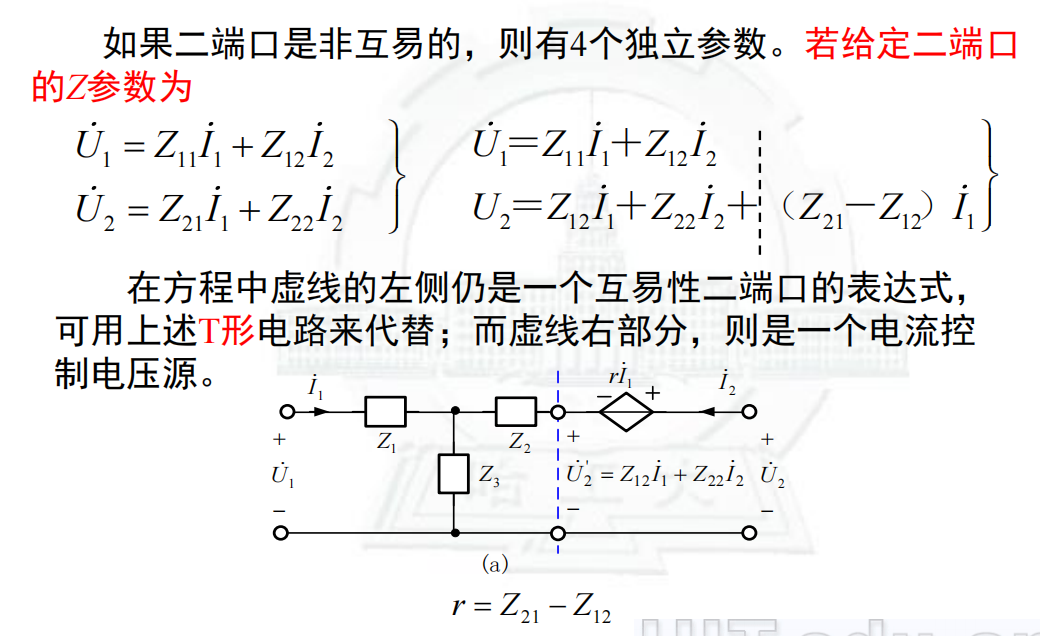
\includegraphics[width=0.6\textwidth]{10.4.1.png}\par
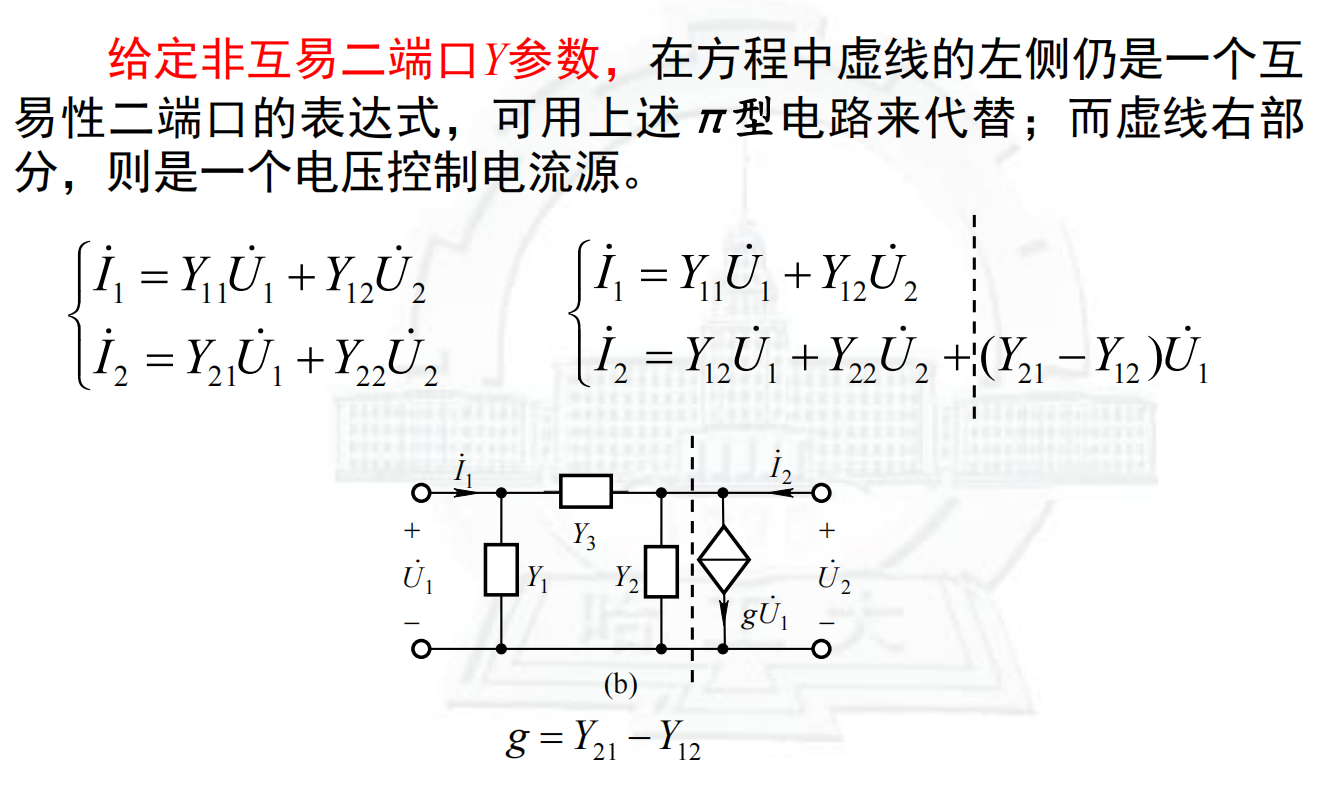
\includegraphics[width=0.6\textwidth]{10.4.2.png}\par

\section{二端口网络与电源和负载的连接}
\subsection{输入阻抗、输出阻抗}
输入阻抗。

特性阻抗（不做要求）。

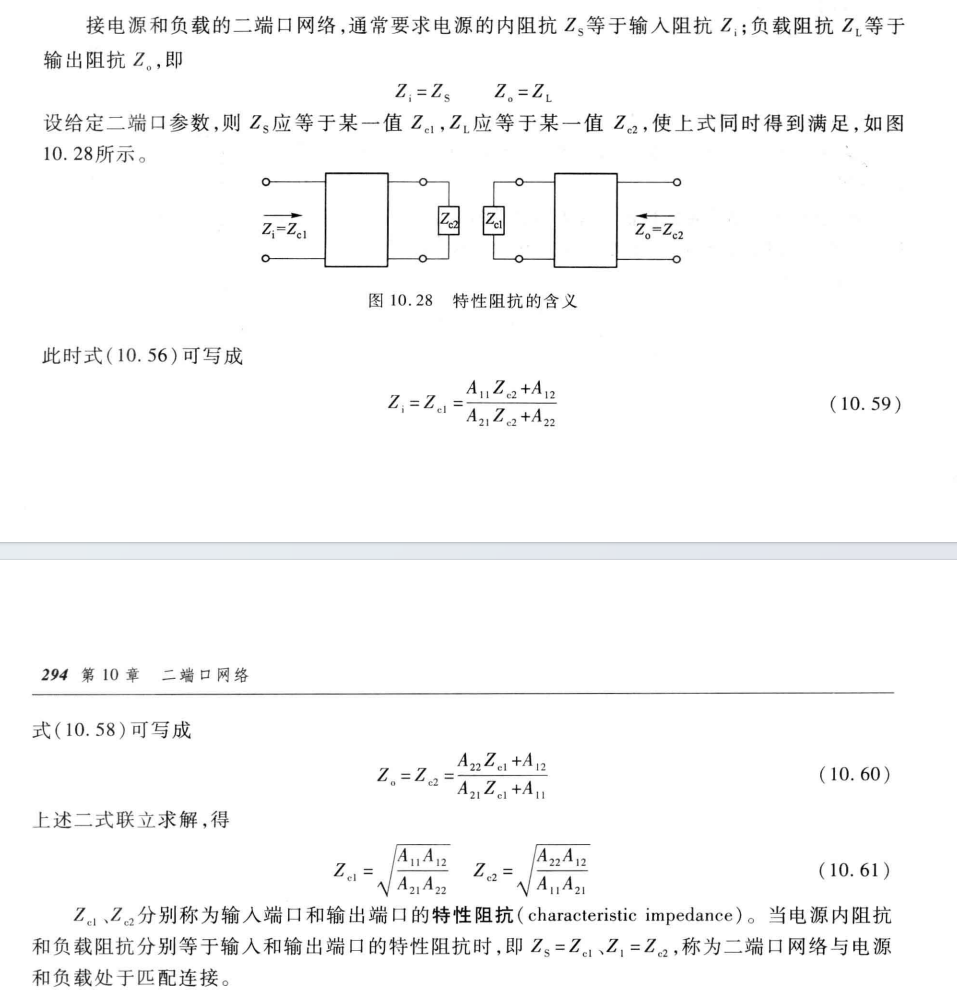
\includegraphics[width=0.6\textwidth]{10.3.png}\par

对称二端口网络的传输系数和特性阻抗。

\section{二端口网络的级联}

\endinput

% 电路与电子学III 课程笔记 —— 第十二章（教材第12章）非线性电阻电路
\chapter{非线性电阻电路}

\section{非线性电阻元件的特性}

含有非线性元件的电路，其电路方程是非线性的，这种电路称为\textbf{非线性电路}。非线性电路广泛存在：
一方面是某些元件不可避免的非线性特性（如二极管、晶体管），另一方面是人为设计的非线性电路，
用以实现线性电路无法实现的功能。分析非线性电路要比分析线性电路复杂得多，
\textbf{基于线性方程的各种电路定理不能直接用于非线性电路}。作为基础，本章研究最简单的非线性电路
——非线性电阻电路。

\subsection{定义与典型特性}
非线性电阻元件的\textbf{约束方程是非线性的}：其电压、电流关系不是通过 $u-i$ 平面坐标原点的直线，
因而不满足欧姆定律，只能写成
\begin{equation}
  u=f(i)\qquad\text{或}\qquad i=g(u)
\end{equation}
例如半导体 PN 结二极管，根据半导体物理可得其电压、电流的解析关系为
\begin{keyformula}{i=I_S\left(\mathrm{e}^{u/U_T}-1\right)}
\end{keyformula}
式中 $I_S$ 为反向饱和电流，$U_T$ 为温度电压当量，二者在二极管型号与工作温度一定时都是常量
（室温下 $U_T\approx26\ \mathrm{mV}$）。加正向电压时特性基本按指数规律上升；加反向电压时
$\mathrm{e}^{u/U_T}$ 很快趋于零，电流近似等于 $-I_S$（很小的量）。任何元件的数学模型都有适用范围：
当反向电压超过反向击穿电压（$|u|>|U_{BR}|$）时，反向电流急剧增加，不再遵循该解析式。

实际上多数非线性电阻元件难以从理论上得出解析表达式，通常只能用\textbf{曲线或数据表}描述。

\subsection{按控制量分类}
\begin{itemize}
  \item \textbf{单调型}：$u$ 与 $i$ 互为单值函数（如 PN 结二极管），$u=u(i)$ 与 $i=i(u)$ 都可单值表示。
  \item \textbf{流控型}（current controlled）：$u$ 是 $i$ 的单值函数，记作 $u=u(i)$；而同一电压下电流可能出现
        多值，即其反函数是多值函数。典型例子是辉光管，其特性在第 I 象限呈“S”形。
  \item \textbf{压控型}（voltage controlled）：$i$ 是 $u$ 的单值函数，记作 $i=i(u)$；而同一电流下电压可能多值。
        典型例子是隧道二极管，其特性在第 I 象限呈“N”形。
\end{itemize}
区分单调型、压控型和流控型的主要原因是：\textbf{对不同类型要选用不同的方法列写电路方程}
（流控型取 $i$ 为变量，压控型取 $u$ 为变量）。

\subsection{双向性与方向性}
线性电阻没有方向性，其特性曲线对称于坐标原点，具有\textbf{双向性}，使用时不必考虑极性。
有些非线性电阻（如辉光管）的特性仍是双向的，即 $-u=u(-i)$；而 PN 结二极管、隧道二极管
\textbf{有方向性}，正向与反向的导电性不同，特性曲线对原点不对称，电路符号上有明显的方向标志，
使用时应按方向正确连接。

\subsection{静态电阻与动态电阻}
非线性电阻的电阻值不是常数，随工作点而变，必须区分两种“电阻”：
\begin{keyformula}{R=\frac{u}{i}\ \ (\text{\songti 静态电阻}),\qquad
  R_d=\frac{\mathrm{d}u}{\mathrm{d}i}\ \ (\text{\songti 动态电阻})}
\end{keyformula}
静态电阻 $R$ 是工作点与原点连线的斜率的倒数，反映该工作点上的整体伏安关系；
动态电阻 $R_d$（又称增量电阻、微变电阻）是特性曲线在该点切线的斜率，反映工作点附近的局部变化关系。
同理有静态电导 $G=i/u$ 与动态电导 $G_d=\mathrm{d}i/\mathrm{d}u=1/R_d$。
$R$ 恒为正，而 $R_d$ \textbf{可以为负}（S 形、N 形特性的下降段），负动态电阻向电路提供能量。

\begin{corepoint}{静态电阻与动态电阻一般\textbf{不相等}，只有线性电阻（特性为过原点的直线）二者才相等。
易错点：小信号分析中用的是\textbf{动态电阻} $R_d$，而算工作点功率、效率时用\textbf{静态电阻}（即 $U_Q/I_Q$）。
图中“切线斜率”的取法：$R_d=\mathrm{d}u/\mathrm{d}i$，斜率越大动态电阻越大，切勿取倒数。}
\end{corepoint}

\section{非线性直流电路方程}

电路方程决定于\textbf{结构约束}和\textbf{支路约束}：前者即基尔霍夫定律方程，它们不涉及元件性质，
总是线性代数方程；后者取决于支路中的元件，若存在非线性电阻，就会出现非线性代数方程。因此
\textbf{叠加定理、齐性原理、戴维南定理、诺顿定理等不能直接用于解非线性电路}。

实际电路中常是线性元件与非线性元件同时存在，往往可以先把线性部分尽量划分出来加以等效化简，
以便建立尽可能简单的非线性电路方程。

\subsection{只含一个非线性电阻时的求解步骤}
若电路只含一个非线性电阻且主要关心它的解答，可把电路划分为\textbf{线性部分}和\textbf{非线性部分}：
\begin{enumerate}
  \item 利用线性电路的戴维南定理（或诺顿定理）对线性部分等效化简，得到只含一个电压源 $U_{OC}$、
        一个等效电阻 $R$ 与非线性电阻串联的简单电路；
  \item 列写该电路方程：若为\textbf{流控型}（$u=u(i)$），以电流 $i$ 为变量列 KVL
        \begin{equation}
          Ri+u(i)=U_{OC}
          \label{eq:ch12-flow}
        \end{equation}
        若为\textbf{压控型}（$i=i(u)$），以电压 $u$ 为变量列 KVL
        \begin{equation}
          Ri(u)+u=U_{OC}
          \label{eq:ch12-volt}
        \end{equation}
  \item 求解式 \eqref{eq:ch12-flow} 或 \eqref{eq:ch12-volt}，得到非线性电阻上的解答 $(U,I)$；
  \item 若还要进一步求线性部分的解答，可用电压源或电流源\textbf{置换}非线性电阻（置换定理），
        得到线性直流电路再求解。
\end{enumerate}

\subsection{含多个非线性电阻时的方程列写}
若电路含有较多的非线性电阻，或需要计算较多的电压、电流，则宜对电路列写联立方程组：
用节点电压法或回路电流法把结构约束写成线性方程，再把各非线性电阻的支路约束代入，
得到\textbf{非线性代数方程组}。这类方程组一般没有解析解，需用下一节的数值方法求解。

\begin{corepoint}{非线性电路的三个关键差别：\textbf{（1）}不能叠加，故“分别求各电源作用再相加”失效；
\textbf{（2）}解可能不唯一（多个工作点），必须逐个检验其物理合理性（如功率、是否落在特性曲线的适用段内）；
\textbf{（3）}“线性部分可用戴维南定理等效”与“戴维南定理可用于非线性电路”是两回事——前者成立，
因为等效只涉及线性部分；后者不成立。}
\end{corepoint}

\section{数值分析法}

求解非线性电路归结为求非线性方程（组）的根，一般不易求解析解，常用数值分析法，
其中最基本的是\textbf{牛顿—拉夫逊法}（切线法）。

\subsection{牛顿—拉夫逊迭代公式}
设要求解方程 $f(x)=0$，取初值 $x_0$，迭代公式为
\begin{keyformula}{x_{k+1}=x_k-\frac{f(x_k)}{f'(x_k)},\qquad k=0,1,2,\cdots}
\end{keyformula}
其几何意义是：在点 $(x_k,f(x_k))$ 处作曲线 $f(x)$ 的切线，以切线与横轴的交点作为下一次的近似值 $x_{k+1}$。
当 $|x_{k+1}-x_k|$ 小于规定容许误差 $\varepsilon$ 时停止迭代，取 $x_{k+1}$ 为解。

\subsection{应用于非线性电阻电路}
以含二极管的电路为例，回路电压方程为
\begin{equation}
  u_R+u-U_S=RI+u-U_S=0
\end{equation}
将二极管的特性 $i=I_S(\mathrm{e}^{u/U_T}-1)$ 代入，得到关于 $u$ 的非线性方程
\begin{equation}
  f(u)=RI_S\left(\mathrm{e}^{u/U_T}-1\right)+u-U_S=0
\end{equation}
其导数 $f'(u)=R\dfrac{I_S}{U_T}\mathrm{e}^{u/U_T}+1$，代入迭代公式即可逐次逼近。若特性以多项式给出，
也可直接求多项式的根（如 MATLAB 的 \texttt{roots}）。

\subsection{收敛性与注意点}
牛顿法收敛快（平方收敛），但有条件：\textbf{初值须在真解附近}，且迭代过程中 $f'(x_k)\ne0$；
若初值选得不好或曲线有拐点，迭代可能发散或振荡。改善办法：选取合理初值（如用图解法定出大致位置）、
限制每次修正量（阻尼）、改用弦截法或二分法等。

\begin{corepoint}{数值法的答案必须\textbf{回代检验}：把求得的 $(U,I)$ 代回原方程，残差应小于容许误差。
另外多解时不能只报第一个收敛值——非线性电路常有两个甚至三个工作点，需按物理意义（如
$u$ 是否在特性曲线适用范围内、功率是否为负）取舍。}
\end{corepoint}

\section{分段线性近似法}

非线性电阻元件的特性通常可以测定其电压、电流特性曲线，但有时不能找出它的解析表达式。
此时可用若干段直线去逼近该曲线，每一段直线对应一个线性方程，从而把非线性问题化为一系列线性问题，
这种方法称为\textbf{分段线性近似法}。

\subsection{折线的数学表示}
把特性曲线分成若干区段，第 $k$ 段用直线近似：
\begin{keyformula}{u=R_{dk}i+U_{0k}\qquad\text{或}\qquad i=G_{dk}u+I_{0k}}
\end{keyformula}
其中 $R_{dk}=\Delta u/\Delta i$ 是该段的\textbf{动态电阻}（斜率的倒数），$U_{0k}$ 是该段直线在电压轴上的
截距。因此每一段都可等效为一个动态电阻与一个电压源（或动态电导与一个电流源）的串联（并联）组合。

\subsection{求解步骤}
\begin{enumerate}
  \item 把每个非线性电阻的特性曲线用折线近似，确定各段的 $R_{dk}$、$U_{0k}$；
  \item 对每个非线性电阻\textbf{假定它工作在某一区段}，用该段的线性模型替代它，得到相应的线性电路；
  \item 解这个线性电路，求出各非线性电阻的电压、电流；
  \item \textbf{检验}：所得工作点是否落在所假定的区段内。若全部符合，则该解有效；
        否则换一种区段组合重新计算。
\end{enumerate}
当电路含多个非线性电阻时，区段组合有多种，只有各非线性电阻的解都落在各自假定的区段内，
该组合才是自洽的；因此可能得到多组自洽解，即多个工作点。

\subsection{特点}
优点是每一段都是线性电路，可直接搬用线性电路的一切方法（等效、节点法、回路法），且能处理多值特性、
便于求多个工作点；缺点是折线近似带来误差，区段组合多时试算量大。

\begin{corepoint}{分段线性法的核心是\textbf{“假定—求解—校验”}三步闭环，校验一步不能省：
算出的工作点若越出假定区段，说明该解无效，必须换组合重算。常见错误是算出一个答案就直接写结论，
而该点其实落在折线的另一段上。}
\end{corepoint}

\section{图解法}

当非线性电阻的特性以曲线给出时，可直接用作图法求工作点，物理概念直观。

\subsection{曲线相交法（负载线法）}
把非线性电阻以外的线性部分等效为 $U_{OC}$ 与 $R$ 串联，其外特性为
\begin{equation}
  u=U_{OC}-Ri
\end{equation}
这是一条斜率为 $-R$、在电压轴上截距为 $U_{OC}$ 的直线，称为\textbf{负载线}。把它与非线性电阻的
$u-i$ 特性曲线画在同一坐标系中，\textbf{两曲线的交点即为工作点} $(U,I)$：交点同时满足线性部分的外特性
与非线性元件的特性。

\subsection{曲线相加法}
当电路含多个非线性电阻时，可用曲线相加求等效特性：
\begin{itemize}
  \item \textbf{串联}：各元件电流相同，故在同一电流下把各元件的电压相加，得等效特性 $u(i)=u_1(i)+u_2(i)$；
  \item \textbf{并联}：各元件电压相同，故在同一电压下把各元件的电流相加，得等效特性 $i(u)=i_1(u)+i_2(u)$。
\end{itemize}
求出等效特性后，再与线性部分的负载线相交，即得工作点；必要时逐级回代求各元件的电压、电流。

\subsection{适用范围}
图解法适用于特性曲线已知且（在所讨论区段内）为单值的情形，对单调型、流控型、压控型都可使用，
只需注意相加时选对公共变量。其缺点是精度受作图与读数限制，多解时需仔细辨认各交点。

\begin{corepoint}{作图法的两个易错点：\textbf{（1）}串联相加时保持\textbf{电流}相同、把\textbf{电压}相加；
并联相加时保持\textbf{电压}相同、把\textbf{电流}相加——公共变量选错则曲线全错。
\textbf{（2）}负载线的斜率是 $-R$ 而不是 $R$，截距是 $U_{OC}$（开路电压），不要与短路电流混淆。}
\end{corepoint}

\section{小信号分析法}

工程上常见这样的情况：非线性电阻上除直流偏置（大信号）外，还叠加了一个幅度很小的交流信号。
此时可在直流工作点附近把特性\textbf{线性化}，用小信号分析法求解。

\subsection{基本原理}
设直流电源单独作用时，非线性电阻工作在\textbf{静态工作点} $Q(U_Q,I_Q)$；再叠加小信号 $\Delta u_S$ 后，
工作点在其附近微小变动。把特性 $i=i(u)$ 在 $Q$ 点作泰勒展开并只取一阶项：
\begin{equation}
  i\approx i(U_Q)+\left.\frac{\mathrm{d}i}{\mathrm{d}u}\right|_{Q}\Delta u
  =I_Q+G_d\Delta u
\end{equation}
即小信号分量之间满足线性关系
\begin{keyformula}{\Delta i=G_d\Delta u,\qquad \Delta u=R_d\Delta i,\qquad
  R_d=\left.\frac{\mathrm{d}u}{\mathrm{d}i}\right|_{Q}}
\end{keyformula}
其中 $R_d$ 是工作点 $Q$ 处的\textbf{动态电阻}。

\subsection{小信号等效电路与解题步骤}
\begin{enumerate}
  \item 令小信号源为零，求出直流工作点 $Q(U_Q,I_Q)$（用前几节的方法）；
  \item 在 $Q$ 点求动态电阻 $R_d=\left.\dfrac{\mathrm{d}u}{\mathrm{d}i}\right|_{Q}$（由特性曲线切线或解析式求导）；
  \item 画\textbf{小信号等效电路}：原电路拓扑不变，直流电源置零（电压源短路、电流源开路），
        非线性电阻用 $R_d$ 替代，只保留小信号源；
  \item 用线性电路方法求小信号响应 $\Delta u$、$\Delta i$；
  \item 叠加得全解：$u=U_Q+\Delta u$，$i=I_Q+\Delta i$。
\end{enumerate}

\subsection{适用条件}
小信号分析法成立的条件是：\textbf{（1）}特性在 $Q$ 点附近连续可导；\textbf{（2）}小信号幅度足够小，
使二阶及以上的高阶项可以忽略。它把非线性问题化为“直流工作点 $+$ 线性小信号”两步，是电子线路
（放大器、二极管检波等）分析的基本方法。

\begin{corepoint}{小信号等效电路中\textbf{直流电源必须置零}、非线性电阻必须换成\textbf{动态电阻}
（而不是静态电阻 $U_Q/I_Q$），这是两个最常见的错误。若特性下降段 $R_d<0$，等效电路中就出现负电阻，
这并非算错。最后回答问题时要把静态量与信号量分别写清，不可混为一个表达式。}
\end{corepoint}

\section{本章小结}
\begin{enumerate}
  \item 非线性电阻的电压、电流关系不满足欧姆定律，其约束方程是非线性的（解析式、曲线或数据表）。
        按控制量分为单调型、流控型（$u=u(i)$ 单值，如辉光管）和压控型（$i=i(u)$ 单值，如隧道二极管）；
        按对称性分为双向性与有方向性的元件。
  \item 非线性电阻有静态电阻 $R=u/i$ 与动态电阻 $R_d=\mathrm{d}u/\mathrm{d}i$ 之分，后者可为负值。
  \item 非线性电路的结构约束仍是线性方程，但支路约束是非线性的，故整体方程为非线性代数方程；
        叠加定理、齐性原理、戴维南定理等不能直接使用，但可对\textbf{线性部分}作等效化简。
  \item 只含一个非线性电阻时，可按“划分线性/非线性—线性部分等效—按控制类型列方程—求解—置换求其余量”
        的步骤处理。
  \item 数值分析法以牛顿—拉夫逊法为代表：$x_{k+1}=x_k-f(x_k)/f'(x_k)$，收敛快但对初值敏感，
        结果须回代检验。
  \item 分段线性近似法用折线代替曲线，每段 $u=R_{dk}i+U_{0k}$，按“假定区段—解线性电路—校验”闭环进行，
        可求出多个工作点。
  \item 图解法用负载线 $u=U_{OC}-Ri$ 与特性曲线求交点；多非线性电阻时用曲线相加（串联加电压、
        并联加电流）求等效特性。
  \item 小信号分析法在工作点处线性化：$\Delta u=R_d\Delta i$，$R_d$ 为 $Q$ 点的动态电阻；
        小信号等效电路中直流电源置零、非线性电阻用 $R_d$ 替代，全解为静态量与信号量之和。
\end{enumerate}

\endinput

% 电路与电子学III 课程笔记 —— 第十三章（教材第13章）均匀传输线
\chapter{均匀传输线}

\section{均匀传输线及其方程}

\subsection{电路参数的分布性}
本章之前研究的都是\textbf{集中参数电路}：认为各种电路参数（电阻、电感和电容）都集中在某些元件上，
各元件之间用理想导线相连。然而任何实际电路的参数都是分布的——电感线圈的电感分布在它的每一线匝上，
实际电阻器的电阻分布在它的全部长度上。建立集中参数模型时忽略了参数的分布性，用集中参数元件近似表示其作用。

根据电磁场理论，当电路器件尺寸远小于其工作频率 $f$ 下的电磁波波长 $\lambda$（$v$ 为电磁波波速，
对于架空线接近光速）时，用集中参数模型分析可以满足实际要求。例如工频 $f=50\ \mathrm{Hz}$ 对应的
波长约 $6000\ \mathrm{km}$，常见工频电路器件尺寸远小于该长度，故一般工频电路可按集中参数处理。
集中参数电路中只涉及元件端子上的电磁量，这些电磁量与空间坐标无关。

若实际电路尺寸可与波长相比甚至大于波长，就必须考虑参数的分布性：
\begin{itemize}
  \item 长距离电力输电线：$500\ \mathrm{km}$ 与 $6000\ \mathrm{km}$ 相比已不算小，需考虑参数分布性；
  \item 高频通信线路：$f=300\ \mathrm{MHz}$ 时波长仅 $1\ \mathrm{m}$，器件尺寸接近甚至超过波长，
        必须用分布参数电路分析。
\end{itemize}

\subsection{均匀传输线的原参数}
由两根连续导体（往返两导线）构成的传输线，若其\textbf{电阻、电感、电容和漏电导沿全线均匀分布}，
则称为\textbf{均匀传输线}。用四个\textbf{原参数}（单位长度的参数）描述：
\begin{table}[htbp]
  \centering
  \renewcommand{\tablename}{表}%
  \caption{均匀传输线的四个原参数（单位长度值）}
  \begin{tabular}{llll}
    \toprule
    参数 & 名称 & 单位 & 物理含义 \\
    \midrule
    $R_0$ & 单位长度电阻 & $\Omega/\mathrm{m}$ & 导线发热损耗 \\
    $L_0$ & 单位长度电感 & $\mathrm{H/m}$ & 导线周围磁场储能 \\
    $G_0$ & 单位长度漏电导 & $\mathrm{S/m}$ & 绝缘介质漏电损耗 \\
    $C_0$ & 单位长度电容 & $\mathrm{F/m}$ & 导线间电场储能 \\
    \bottomrule
  \end{tabular}
\end{table}

\subsection{传输线方程}
在距始端 $x$ 处取长度 $\mathrm{d}x$ 的微段，其电阻为 $R_0\mathrm{d}x$、电感为 $L_0\mathrm{d}x$，
两线间漏电导为 $G_0\mathrm{d}x$、电容为 $C_0\mathrm{d}x$。对该微段列 KVL 与 KCL，
并忽略二阶无穷小量，得\textbf{均匀传输线方程}（电报方程）
\begin{keyformula}{-\frac{\partial u}{\partial x}=R_0i+L_0\frac{\partial i}{\partial t},\qquad
  -\frac{\partial i}{\partial x}=G_0u+C_0\frac{\partial u}{\partial t}}
\end{keyformula}
式中 $u=u(x,t)$、$i=i(x,t)$ 既是时间 $t$ 的函数，又是位置 $x$ 的函数——这正是分布参数电路的本质特征：
电压、电流沿线各点不同。方程左端的负号表示电压、电流随 $x$ 增加而减小（能量沿 $x$ 方向传输）。

\begin{corepoint}{原参数是“单位长度”的量，单位为 $\Omega/\mathrm{m}$、$\mathrm{H/m}$、$\mathrm{S/m}$、$\mathrm{F/m}$，
全线的总参数则为 $R_0l$、$L_0l$、$G_0l$、$C_0l$。分布参数电路与集中参数电路的根本区别是
\textbf{电压、电流是空间坐标的函数}，因此必须用偏微分方程描述。}
\end{corepoint}

\section{均匀传输线方程的正弦稳态解}

\subsection{相量形式的方程}
设均匀线由正弦电源激励，达到稳态后线路上任一点的电压、电流都是同一频率的正弦量，可用相量表示：
\begin{equation}
  u(x,t)=\mathrm{Re}\left[\sqrt2\dot{U}(x)\mathrm{e}^{\mathrm{j}\omega t}\right],\qquad
  i(x,t)=\mathrm{Re}\left[\sqrt2\dot{I}(x)\mathrm{e}^{\mathrm{j}\omega t}\right]
\end{equation}
代入传输线方程，偏导数变为对 $x$ 的全导数，得
\begin{keyformula}{-\frac{\mathrm{d}\dot{U}(x)}{\mathrm{d}x}=Z_0\dot{I}(x),\qquad
  -\frac{\mathrm{d}\dot{I}(x)}{\mathrm{d}x}=Y_0\dot{U}(x)}
\end{keyformula}
其中 $Z_0=R_0+\mathrm{j}\omega L_0$ 为单位长度阻抗，$Y_0=G_0+\mathrm{j}\omega C_0$ 为单位长度导纳。
再对 $x$ 求导一次，得
\begin{equation}
  \frac{\mathrm{d}^2\dot{U}(x)}{\mathrm{d}x^2}=Z_0Y_0\dot{U}(x)=\gamma^2\dot{U}(x),\qquad
  \frac{\mathrm{d}^2\dot{I}(x)}{\mathrm{d}x^2}=\gamma^2\dot{I}(x)
\end{equation}
\begin{keyformula}{\gamma=\sqrt{Z_0Y_0}=\sqrt{\left(R_0+\mathrm{j}\omega L_0\right)\left(G_0+\mathrm{j}\omega C_0\right)}
  =\alpha+\mathrm{j}\beta}
\end{keyformula}
$\gamma$ 是由线路原参数和频率决定的复常数，称为线路的\textbf{传播常数}；实部 $\alpha$ 称为
\textbf{衰减常数}，虚部 $\beta$ 称为\textbf{相位常数}，二者都具有倒长度的量纲（$1/\mathrm{m}$）。

\subsection{通解与特性阻抗}
方程的通解为
\begin{equation}
  \dot{U}(x)=A_1\mathrm{e}^{-\gamma x}+A_2\mathrm{e}^{\gamma x},\qquad
  \dot{I}(x)=B_1\mathrm{e}^{-\gamma x}+B_2\mathrm{e}^{\gamma x}
\end{equation}
由 $-\dfrac{\mathrm{d}\dot{U}}{\mathrm{d}x}=Z_0\dot{I}$ 得
$\dot{I}=\dfrac{\gamma}{Z_0}\left(A_1\mathrm{e}^{-\gamma x}-A_2\mathrm{e}^{\gamma x}\right)$，令
\begin{keyformula}{Z_c=\frac{Z_0}{\gamma}=\sqrt{\frac{Z_0}{Y_0}}
  =\sqrt{\frac{R_0+\mathrm{j}\omega L_0}{G_0+\mathrm{j}\omega C_0}}}
\end{keyformula}
$Z_c$ 称为\textbf{特性阻抗}或\textbf{波阻抗}，具有电阻的量纲，只与线路原参数和频率有关，即
\begin{equation}
  \dot{I}(x)=\frac{A_1}{Z_c}\mathrm{e}^{-\gamma x}-\frac{A_2}{Z_c}\mathrm{e}^{\gamma x}
\end{equation}

\subsection{由始端条件确定的解}
以始端为计算距离的起点（$x=0$ 处 $\dot{U}=\dot{U}_1$、$\dot{I}=\dot{I}_1$），可定出积分常数
$A_1=\tfrac12(\dot{U}_1+Z_c\dot{I}_1)$、$A_2=\tfrac12(\dot{U}_1-Z_c\dot{I}_1)$，代回并用双曲函数
$\cosh\gamma x=\tfrac12(\mathrm{e}^{\gamma x}+\mathrm{e}^{-\gamma x})$、
$\sinh\gamma x=\tfrac12(\mathrm{e}^{\gamma x}-\mathrm{e}^{-\gamma x})$，得
\begin{keyformula}{\dot{U}(x)=\dot{U}_1\cosh\gamma x-\dot{I}_1Z_c\sinh\gamma x,\qquad
  \dot{I}(x)=-\frac{\dot{U}_1}{Z_c}\sinh\gamma x+\dot{I}_1\cosh\gamma x}
\end{keyformula}
写成矩阵形式
\begin{equation}
  \begin{bmatrix}\dot{U}(x)\\ \dot{I}(x)\end{bmatrix}
  =\begin{bmatrix}\cosh\gamma x & -Z_c\sinh\gamma x\\
    -\dfrac{1}{Z_c}\sinh\gamma x & \cosh\gamma x\end{bmatrix}
  \begin{bmatrix}\dot{U}_1\\ \dot{I}_1\end{bmatrix}
\end{equation}
令 $x=l$（线路长度）即得终端电压、电流。

\subsection{由终端条件确定的解}
若已知终端电压 $\dot{U}_2$、电流 $\dot{I}_2$，在 $x=l$ 处代入上式并对 $\dot{U}_1$、$\dot{I}_1$ 求解，
计及 $\cosh^2\gamma l-\sinh^2\gamma l=1$，得
\begin{keyformula}{\dot{U}_1=\dot{U}_2\cosh\gamma l+\dot{I}_2Z_c\sinh\gamma l,\qquad
  \dot{I}_1=\frac{\dot{U}_2}{Z_c}\sinh\gamma l+\dot{I}_2\cosh\gamma l}
\end{keyformula}
矩阵形式为
\begin{equation}
  \begin{bmatrix}\dot{U}_1\\ \dot{I}_1\end{bmatrix}
  =\begin{bmatrix}\cosh\gamma l & Z_c\sinh\gamma l\\
    \dfrac{1}{Z_c}\sinh\gamma l & \cosh\gamma l\end{bmatrix}
  \begin{bmatrix}\dot{U}_2\\ \dot{I}_2\end{bmatrix}
\end{equation}
这正是把均匀线视为一个二端口网络时的\textbf{传输参数方程}，传输参数矩阵为
\begin{equation}
  \boldsymbol{A}=\begin{bmatrix}\cosh\gamma l & Z_c\sinh\gamma l\\
    \dfrac{1}{Z_c}\sinh\gamma l & \cosh\gamma l\end{bmatrix}
\end{equation}
其中 $A_{11}=A_{22}=\cosh\gamma l$，$\det\boldsymbol{A}=1$，说明均匀传输线是一个\textbf{对称二端口网络}
——对调输入、输出端不会改变其端口特性。

若以\textbf{终端为坐标原点}、向始端方向为距离 $x'$ 的正方向，则只需把上式中的 $l$ 改为 $x'$，
即得距终端 $x'$ 处的电压、电流：
\begin{equation}
  \dot{U}(x')=\dot{U}_2\cosh\gamma x'+\dot{I}_2Z_c\sinh\gamma x',\qquad
  \dot{I}(x')=\frac{\dot{U}_2}{Z_c}\sinh\gamma x'+\dot{I}_2\cosh\gamma x'
\end{equation}

\begin{corepoint}{两套公式极易混用：\textbf{以始端为原点}时 $x$ 从始端算起，公式中 $\dot{U}_1$ 前取“$+$”、
$\dot{I}_1Z_c$ 前取“$-$”；\textbf{以终端为原点}时 $x'$ 从终端算起，两项都取“$+$”。
做题先明确坐标原点与已知量位置，再选对应公式，切勿张冠李戴。}
\end{corepoint}

\section{均匀传输线上的行波}

\subsection{正向行波与反向行波}
把通解改写为两个分量之和：
\begin{equation}
  \dot{U}(x)=\underbrace{A_1\mathrm{e}^{-\gamma x}}_{\dot{U}^+(x)}
  +\underbrace{A_2\mathrm{e}^{\gamma x}}_{\dot{U}^-(x)},\qquad
  \dot{I}(x)=\underbrace{\frac{A_1}{Z_c}\mathrm{e}^{-\gamma x}}_{\dot{I}^+(x)}
  -\underbrace{\frac{A_2}{Z_c}\mathrm{e}^{\gamma x}}_{\dot{I}^-(x)}
\end{equation}
设 $A_1=U'\mathrm{e}^{\mathrm{j}\psi'}$，则正向电压行波的瞬时值为
\begin{equation}
  u^+(x,t)=\mathrm{Re}\left[\sqrt2\dot{U}^+(x)\mathrm{e}^{\mathrm{j}\omega t}\right]
  =\sqrt2U'\mathrm{e}^{-\alpha x}\cos\left(\omega t-\beta x+\psi'\right)
\end{equation}
它表明：沿 $x$ 方向传播的\textbf{正向行波}（入射波）振幅按 $\mathrm{e}^{-\alpha x}$ 衰减，相位随 $x$
滞后 $\beta x$。同理 $\dot{U}^-(x)$ 对应沿 $-x$ 方向传播的\textbf{反向行波}（反射波）。

\subsection{相速与波长}
设某相位点满足 $\omega t-\beta x+\psi'=$ 常数，对时间求导得
\begin{keyformula}{v_p=\frac{\omega}{\beta}\ \ (\text{\songti 相速}),\qquad
  \lambda=\frac{2\pi}{\beta}=\frac{v_p}{f}=v_pT\ \ (\text{\songti 波长})}
\end{keyformula}
相速 $v_p$ 是等相位点移动的速度；波长 $\lambda$ 是同一时刻相位相差 $2\pi$ 的两点间距离，
也等于一个周期内波传播的距离。

\subsection{波阻抗的物理意义}
由通解可见
\begin{keyformula}{\frac{\dot{U}^+(x)}{\dot{I}^+(x)}=\frac{\dot{U}^-(x)}{-\dot{I}^-(x)}=Z_c}
\end{keyformula}
即\textbf{波阻抗等于正向行波的电压与电流之比}（对反向行波则差一负号，因为反射波电流方向与正方向相反）。
$Z_c=|Z_c|\angle\varphi_c$ 一般为复数，其模反映电压波与电流波的幅值比，其辐角表示二者的相位差。

\subsection{反射与终端匹配}
设终端接负载 $Z_L$，则 $\dot{U}_2/\dot{I}_2=Z_L$。由终端处的通解可解出反向行波与正向行波之比，
得\textbf{终端反射系数}
\begin{keyformula}{N_2=\frac{\dot{U}_2^-}{\dot{U}_2^+}=\frac{\dot{I}_2^-}{\dot{I}_2^+}
  =\frac{Z_L-Z_c}{Z_L+Z_c}}
\end{keyformula}
它是一个与负载阻抗有关的复数。
\begin{itemize}
  \item 若 $Z_L=Z_c$，则 $N_2=0$，线路上\textbf{只有正向行波、没有反射波}，这种工作状态称为
        \textbf{负载与传输线匹配}（无反射工作状态）。此时线路上任一处电压与电流相量之比都等于 $Z_c$，
        沿线电压、电流有效值按指数规律单调衰减：
        \begin{equation}
          U(x)=U_1\mathrm{e}^{-\alpha x},\qquad I(x)=I_1\mathrm{e}^{-\alpha x}
        \end{equation}
  \item 若 $Z_L\ne Z_c$，则 $N_2\ne0$，出现反射波，沿线电压、电流是入射波与反射波的叠加，
        其有效值不再单调衰减，可能出现局部升高（驻波的前兆）。
\end{itemize}

\subsection{自然功率与输电效率}
线路在无反射条件下工作时，终端负载吸收的功率称为\textbf{自然功率}：
\begin{equation}
  P_2=U_2I_2\cos\varphi_c=\frac{U_2^2}{|Z_c|}\cos\varphi_c
\end{equation}
由于没有反向行波，匹配状态下传输效率很高，一般通信传输线就常处于这种工作状态。
把 $U_2=U_1\mathrm{e}^{-\alpha l}$、$I_2=I_1\mathrm{e}^{-\alpha l}$ 代入，得
\begin{equation}
  P_2=U_1I_1\mathrm{e}^{-2\alpha l}\cos\varphi_c,\qquad
  \eta=\frac{P_2}{P_1}=\mathrm{e}^{-2\alpha l}
\end{equation}
即匹配时输电效率只由衰减常数与线长决定。

\subsection{输入阻抗}
由终端条件公式可得传输线始端的\textbf{输入阻抗}
\begin{keyformula}{Z_i=\frac{\dot{U}_1}{\dot{I}_1}
  =Z_c\frac{Z_L\cosh\gamma l+Z_c\sinh\gamma l}{Z_L\sinh\gamma l+Z_c\cosh\gamma l}}
\end{keyformula}
若 $Z_L=Z_c$，则 $Z_i=Z_c$，与前述一致：匹配时沿线任一点的输入阻抗都等于 $Z_c$。
终端开路（$Z_L\to\infty$）时 $Z_i=Z_c\coth\gamma l$；终端短路（$Z_L=0$）时 $Z_i=Z_c\tanh\gamma l$。
可见二端口（传输线）具有\textbf{变换阻抗}的作用。

\begin{corepoint}{三个易混的量：\textbf{波阻抗} $Z_c$ 只由线路原参数与频率决定，与负载无关；
\textbf{输入阻抗} $Z_i$ 随负载 $Z_L$ 和线长 $l$ 变化；\textbf{负载阻抗} $Z_L$ 是外接的。
反射系数 $N_2$ 的取值范围：匹配时 $0$，终端开路时 $+1$（电压全反射、电流反向抵消），
终端短路时 $-1$（电压反相，电流加倍）。}
\end{corepoint}

\section{无损耗线、驻波}

\subsection{无损耗线的参数}
若 $R_0=0$、$G_0=0$，则称为\textbf{无损耗线}（理想线）。此时
\begin{keyformula}{\gamma=\sqrt{\mathrm{j}\omega L_0\cdot\mathrm{j}\omega C_0}
  =\mathrm{j}\omega\sqrt{L_0C_0}=\mathrm{j}\beta,\qquad
  Z_c=\sqrt{\frac{L_0}{C_0}}\ \ (\text{\songti 纯电阻})}
\end{keyformula}
即 $\alpha=0$、$\beta=\omega\sqrt{L_0C_0}$，波阻抗为纯实数，
相速 $v_p=\dfrac{\omega}{\beta}=\dfrac{1}{\sqrt{L_0C_0}}$，波长 $\lambda=\dfrac{2\pi}{\beta}$。
无损耗线上行波不衰减，只发生相位变化。

\subsection{驻波的形成}
把无损耗线的解写成
\begin{equation}
  \dot{U}(x)=\dot{U}^+\mathrm{e}^{-\mathrm{j}\beta x}+\dot{U}^-\mathrm{e}^{\mathrm{j}\beta x},\qquad
  \dot{I}(x)=\frac{\dot{U}^+}{Z_c}\mathrm{e}^{-\mathrm{j}\beta x}-\frac{\dot{U}^-}{Z_c}\mathrm{e}^{\mathrm{j}\beta x}
\end{equation}
入射波与反射波幅值相等（$|N_2|=1$）时，二者叠加不再是一个行波，而是\textbf{驻波}：
电压、电流的幅值沿线路按正弦规律分布，出现固定不动的\textbf{波腹}（幅值最大处）与\textbf{波节}
（幅值为零处），相邻波节（或波腹）间距为 $\lambda/2$，波节与相邻波腹间距为 $\lambda/4$。

\subsection{终端开路的无损线}
终端开路时 $\dot{I}_2=0$、$N_2=1$。以终端为原点，由终端条件公式得（$\gamma=\mathrm{j}\beta$）
\begin{equation}
  \dot{U}(x')=\dot{U}_2\cos\beta x',\qquad
  \dot{I}(x')=\mathrm{j}\frac{\dot{U}_2}{Z_c}\sin\beta x'
\end{equation}
电压在终端为\textbf{波腹}、电流在终端为\textbf{波节}；距终端 $\lambda/4$ 处电压为波节、电流为波腹。
输入阻抗
\begin{keyformula}{Z_i=-\mathrm{j}Z_c\cot\beta l=-\mathrm{j}Z_c\cot\frac{2\pi l}{\lambda}}
\end{keyformula}
为纯电抗，随线长作周期性变化：$l=\lambda/4$ 时 $Z_i=0$（相当于短路），$l=\lambda/2$ 时
$Z_i\to\infty$（相当于开路）。

\subsection{终端短路的无损线}
终端短路时 $\dot{U}_2=0$、$N_2=-1$，得
\begin{equation}
  \dot{U}(x')=\mathrm{j}\dot{I}_2Z_c\sin\beta x',\qquad
  \dot{I}(x')=\dot{I}_2\cos\beta x'
\end{equation}
此时终端是电压\textbf{波节}、电流\textbf{波腹}，与开路情形正好对偶。输入阻抗
\begin{keyformula}{Z_i=\mathrm{j}Z_c\tan\beta l=\mathrm{j}Z_c\tan\frac{2\pi l}{\lambda}}
\end{keyformula}
$l=\lambda/4$ 时 $Z_i\to\infty$（相当于开路），$l=\lambda/2$ 时 $Z_i=0$（相当于短路）。

\subsection{终端接纯电抗与四分之一波长变换}
终端接纯电抗时 $|N_2|=1$，线上仍形成驻波，只是波腹、波节的位置随负载而移动。
当 $l=\lambda/4$ 时，由输入阻抗公式（$\beta l=\pi/2$）得
\begin{keyformula}{Z_i=\frac{Z_c^2}{Z_L}\qquad\left(l=\frac{\lambda}{4}\right)}
\end{keyformula}
即\textbf{四分之一波长无损线可作阻抗变换器}：把负载阻抗 $Z_L$ 变换为 $Z_c^2/Z_L$，
适当选择 $Z_c$ 便能实现所需的阻抗匹配。这是微波技术中常用的阻抗匹配手段。

\begin{corepoint}{开路、短路两种极端情形要记牢“互换”关系：开路线的输入阻抗为
$-\mathrm{j}Z_c\cot\beta l$，短路线为 $\mathrm{j}Z_c\tan\beta l$，二者相差 $\lambda/4$ 就互换。
驻波与行波的区别：行波沿线幅值单调（或按指数）变化、相位随位置连续滞后；
驻波幅值有固定的波节波腹、各点相位相同或相反。}
\end{corepoint}

\section{均匀传输线的集中参数等效电路}

当无需研究沿线电压、电流的分布，只需计算始端和终端的电压、电流时，可把均匀线视为集中参数的
\textbf{对称二端口网络}，用对称的 \textbf{T 形}或 \textbf{$\Pi$ 形}电路等效。

\subsection{精确等效（双曲函数形式）}
比较 T 形电路的传输参数与式 $\dot{U}_1=\dot{U}_2\cosh\gamma l+\dot{I}_2Z_c\sinh\gamma l$ 等，可得
\begin{keyformula}{\text{\songti T 形：}\ Z=2Z_c\tanh\frac{\gamma l}{2},\quad Y=\frac{\sinh\gamma l}{Z_c};\qquad
  \text{\songti $\Pi$ 形：}\ Z=Z_c\sinh\gamma l,\quad Y=\frac{2}{Z_c}\tanh\frac{\gamma l}{2}}
\end{keyformula}
其中 T 形的 $Z$ 是两串联臂之和（每臂 $Z/2$），$Y$ 是中间并联臂；$\Pi$ 形的 $Z$ 是串联臂，
$Y$ 是两并联臂之和（每臂 $Y/2$）。

\subsection{短线近似（集中参数形式）}
当线路相对波长较短、$|\gamma l|\ll1$ 时，把双曲函数展成级数并只取第一项，得
\begin{keyformula}{Z\approx Z_0l=\left(R_0+\mathrm{j}\omega L_0\right)l,\qquad
  Y\approx Y_0l=\left(G_0+\mathrm{j}\omega C_0\right)l}
\end{keyformula}
即把全线总阻抗、总导纳集中起来：T 形近似为两臂各 $Z/2$、中间并联 $Y$；$\Pi$ 形近似为串联臂 $Z$、
两端并联各 $Y/2$。这就是中等距离输电线（例如工频下 $50\sim100\ \mathrm{km}$ 的架空线路）常用的电路模型。

\subsection{链形电路（仿真线）}
若要更好地模拟均匀线、研究沿线电压电流分布及其暂态过程，可把均匀线等分成 $n$ 段，
每段看成一个二端口网络，各用 T 形或 $\Pi$ 形等效电路代替，得到由许多相同对称二端口级联而成的
\textbf{链形电路}。计算每段等效参数时只需用 $l/n$ 代替原来的 $l$。这种链形电路常用于实验室对实际
均匀线进行仿真研究，称为\textbf{仿真线}或\textbf{人工线}。

\begin{corepoint}{近似等效电路中没有出现频率变量，似乎与频率无关——其实不然：
近似的前提是 $|\gamma l|\ll1$，而 $\gamma$ 中含 $\omega$。线长一定时，等效的近似程度取决于信号频率，
频率越高近似越差。工程上常以 $l<\lambda/10$（或 $l<1000\ \mathrm{km}$ 工频）作为可用集中参数近似的界限。}
\end{corepoint}

\section{无损均匀线方程的通解}

前面讨论的是正弦激励下的稳态。当传输线始端接入任意波形的电源时，需研究无损线的暂态（波）过程。
对无损耗线，传输线方程化为
\begin{equation}
  -\frac{\partial u}{\partial x}=L_0\frac{\partial i}{\partial t},\qquad
  -\frac{\partial i}{\partial x}=C_0\frac{\partial u}{\partial t}
\end{equation}
消去 $i$ 或 $u$，得波动方程
\begin{equation}
  \frac{\partial^2u}{\partial x^2}=\frac{1}{v^2}\frac{\partial^2u}{\partial t^2},\qquad
  v=\frac{1}{\sqrt{L_0C_0}}
\end{equation}
其通解（达朗贝尔解）为
\begin{keyformula}{u(x,t)=f_1\left(t-\frac{x}{v}\right)+f_2\left(t+\frac{x}{v}\right),\qquad
  i(x,t)=\frac{1}{Z_c}\left[f_1\left(t-\frac{x}{v}\right)-f_2\left(t+\frac{x}{v}\right)\right]}
\end{keyformula}
其中 $f_1$ 表示沿 $+x$ 方向以速度 $v$ 传播的\textbf{正向行波}（入射波），$f_2$ 表示沿 $-x$ 方向传播的
\textbf{反向行波}（反射波）；$v=1/\sqrt{L_0C_0}$ 为波的传播速度，
$Z_c=\sqrt{L_0/C_0}$ 为波阻抗。函数 $f_1$、$f_2$ 的具体形式由\textbf{边界条件}（始端电源、终端负载）
与\textbf{初始条件}（$t=0$ 时沿线的电压、电流分布）确定。

\begin{corepoint}{通解中 $f_1\left(t-\frac{x}{v}\right)$ 表示“波形不变、以速度 $v$ 向右平移”，
这是无损耗、无畸变传输的本质。有损耗时波形会畸变、幅值衰减，需用更复杂的解或数值方法。}
\end{corepoint}

\section{无损均匀线上波的发出}

设无限长（或尚未发生反射的）无损线始端在 $t=0$ 时接入电压源 $u_S(t)$，电源内阻为 $R_S$。
由于波尚未到达终端，线路上只有正向行波，始端电压、电流满足
\begin{equation}
  u_S=u_1+R_Si_1,\qquad u_1=Z_ci_1
\end{equation}
解得始端的入射波
\begin{keyformula}{u_1^+=\frac{Z_c}{R_S+Z_c}u_S(t),\qquad i_1^+=\frac{1}{R_S+Z_c}u_S(t)}
\end{keyformula}
该电压波、电流波以速度 $v$ 沿线路向终端传播，$t$ 时刻波前到达 $x=vt$ 处，波前之后各点的电压、电流
分别为上述值（无损耗线不衰减）。例如 $u_S(t)=U_S\varepsilon(t)$ 时，$x<vt$ 区段内
$u=U_SZ_c/(R_S+Z_c)$、$i=U_S/(R_S+Z_c)$，而 $x>vt$ 区段尚未被波及，电压、电流仍为零。

若电源内阻 $R_S=0$（理想电压源直接接入），则 $u_1^+=U_S$、$i_1^+=U_S/Z_c$；
若 $R_S=Z_c$，则 $u_1^+=U_S/2$——这体现了波阻抗对波的“分压”作用：
\textbf{波阻抗就相当于线路对入射波呈现的“负载电阻”}。

\begin{corepoint}{波的发出有两个要点：\textbf{（1）}波以有限速度 $v$ 传播，线路上不同位置的电压、电流
在不同时刻跃变，不能认为“一接通全线同时有电”；\textbf{（2）}始端入射波的幅值由 $R_S$ 与 $Z_c$ 分压决定，
与终端负载无关（终端尚未起作用）。这正是分布参数电路与集中参数电路最直观的差别。}
\end{corepoint}

\section{无损均匀线上波的反射}

\subsection{终端反射系数}
当入射波到达终端，若终端负载 $Z_L\ne Z_c$，则要产生反射波。由终端处电压、电流的连续性
$u_2=u_2^++u_2^-$、$i_2=i_2^+-i_2^-$ 及 $u_2/i_2=Z_L$、$u_2^+/i_2^+=Z_c$，解得终端反射系数
\begin{keyformula}{N_2=\frac{u_2^-}{u_2^+}=\frac{i_2^-}{i_2^+}=\frac{Z_L-Z_c}{Z_L+Z_c}}
\end{keyformula}
它与正弦稳态下的反射系数形式完全相同。

\subsection{三种典型终端}
\begin{table}[htbp]
  \centering
  \renewcommand{\tablename}{表}%
  \caption{无损线三种典型终端的反射情况}
  \begin{tabular}{llll}
    \toprule
    终端情况 & $Z_L$ & 反射系数 $N_2$ & 反射波与终端电压、电流 \\
    \midrule
    匹配 & $Z_c$ & $0$ & 无反射波，$\ u_2=u_2^+$，$i_2=i_2^+$ \\
    开路 & $\infty$ & $+1$ & $u_2^-=u_2^+$，终端电压加倍为 $2u_2^+$，电流为零 \\
    短路 & $0$ & $-1$ & $u_2^-=-u_2^+$，终端电压为零，电流加倍为 $2i_2^+$ \\
    \bottomrule
  \end{tabular}
\end{table}
一般情形下终端电压、电流为 $u_2=(1+N_2)u_2^+$、$i_2=(1-N_2)i_2^+$。

\subsection{多次反射与波的往返}
反射波到达始端后，若始端也不匹配（$R_S\ne Z_c$），则再次发生反射，形成\textbf{多次反射}，
波在两端之间往返传播，每次反射都按相应端的反射系数改变幅值。设线长为 $l$，波单程传播时间为
$\tau=l/v$，则
\begin{itemize}
  \item $t=\tau$ 时入射波到达终端，产生第一次反射波；
  \item $t=2\tau$ 时反射波回到始端，产生第二次反射；
  \item 以后每隔 $\tau$ 时间在两端交替反射一次，直至能量被电阻消耗殆尽而进入稳态。
\end{itemize}
始端反射系数为 $N_1=\dfrac{R_S-Z_c}{R_S+Z_c}$。$N_1N_2=0$（任一端匹配）时只反射一次，
过程最简单；工程上常用终端匹配来消除反射，避免过电压和信号失真。

\subsection{分析方法}
分析波的多次反射常用“\textbf{格形图}”（bounce diagram）：横轴为距离 $x$、纵轴为时间 $t$，
波的传播路径为斜率 $\pm v$ 的折线，每到达边界就按反射系数乘以相应幅值，再把某一位置、某一时刻
所有到达的波叠加，即得该点的电压或电流。这是分析传输线暂态过程最直观的方法。

\begin{corepoint}{反射的三条判据：\textbf{（1）}$N_2>0$（$Z_L>Z_c$）时反射波与入射波同号，
终端电压升高（开路最甚，加倍）；\textbf{（2）}$N_2<0$（$Z_L<Z_c$）时反射波与入射波异号，
终端电压降低（短路时为零，电流加倍）；\textbf{（3）}只有 $Z_L=Z_c$ 才无反射。
工程上为防止开路末端出现过电压，常在终端接匹配电阻或避雷器。}
\end{corepoint}

\section{本章小结}
\begin{enumerate}
  \item 当电路尺寸可与工作频率下的电磁波波长相比时，必须考虑参数的分布性，用分布参数电路分析。
        均匀传输线用四个原参数 $R_0$、$L_0$、$G_0$、$C_0$（单位长度值）描述，其电压、电流是位置与时间的
        二元函数，满足传输线方程 $-\dfrac{\partial u}{\partial x}=R_0i+L_0\dfrac{\partial i}{\partial t}$、
        $-\dfrac{\partial i}{\partial x}=G_0u+C_0\dfrac{\partial u}{\partial t}$。
  \item 正弦稳态下以相量表示，得 $\dfrac{\mathrm{d}\dot{U}}{\mathrm{d}x}=-Z_0\dot{I}$、
        $\dfrac{\mathrm{d}\dot{I}}{\mathrm{d}x}=-Y_0\dot{U}$，其解由传播常数
        $\gamma=\sqrt{Z_0Y_0}=\alpha+\mathrm{j}\beta$ 与特性阻抗 $Z_c=\sqrt{Z_0/Y_0}$ 表征。
  \item 已知始端或终端条件，用双曲函数写出沿线电压、电流的分布；均匀线等效为一个对称二端口网络，
        其传输参数矩阵满足 $A_{11}=A_{22}=\cosh\gamma l$、$\det\boldsymbol{A}=1$。
  \item 沿线电压、电流可分解为正向行波与反向行波；相速 $v_p=\omega/\beta$，波长 $\lambda=v_p/f$，
        波阻抗等于正向行波电压与电流之比；终端反射系数 $N_2=(Z_L-Z_c)/(Z_L+Z_c)$，
        $Z_L=Z_c$ 时匹配、无反射，此时传输的功率称自然功率，效率 $\eta=\mathrm{e}^{-2\alpha l}$。
  \item 无损耗线 $R_0=G_0=0$，$\gamma=\mathrm{j}\beta$、$Z_c=\sqrt{L_0/C_0}$ 为纯电阻，行波不衰减；
        终端开路或短路时形成驻波，输入阻抗为 $-\mathrm{j}Z_c\cot\beta l$ 或 $\mathrm{j}Z_c\tan\beta l$，
        $\lambda/4$ 线可实现阻抗变换 $Z_i=Z_c^2/Z_L$。
  \item 只需计算端量时，可用 T 形或 $\Pi$ 形集中参数等效电路；$|\gamma l|\ll1$ 时
        $Z\approx Z_0l$、$Y\approx Y_0l$，即短线可用集中参数模型。
  \item 无损线暂态过程的通解为 $u=f_1(t-x/v)+f_2(t+x/v)$、
        $i=\left[f_1(t-x/v)-f_2(t+x/v)\right]/Z_c$；始端入射波由 $R_S$ 与 $Z_c$ 分压决定，
        波以速度 $v=1/\sqrt{L_0C_0}$ 传播，在终端按 $N_2$ 反射，可多次反射直至稳态。
\end{enumerate}

\endinput


\end{document}
